\documentclass[a4paper,11pt,fleqn,twoside,openright,final]{memoir}

%%%%%%%%%%%%%%%%%%%%%%%%%%
%% COMMAND DEACTIVATION %%
%%%%%%%%%%%%%%%%%%%%%%%%%%

\let\added\undefined
\let\deleted\undefined


%%%%%%%%%%%%%%
%% PACKAGES %%
%%%%%%%%%%%%%%


%%% Initial things %%%
% Fix various issues with LaTeX2e
\usepackage{fixltx2e}
% Font package
\usepackage{fourier}
% Index
\usepackage{makeidx}
\makeindex


%%% Translations and character encodings %%%
% Enable use of several characters, including æ, ø and å
\usepackage[utf8]{inputenc}
% Danish language
\usepackage[danish]{babel}
% Use PostScript fonts instead of bitmap ones. Also does other stuff.
\usepackage[T1]{fontenc}
% Various LaTeX symbols
\usepackage{latexsym}
% Wider selection of colours
\usepackage{xcolor}
% Improved element justification
\usepackage{ragged2e}
% Font improvements
\usepackage{fix-cm}
% Enables inclusion of PDF files
\usepackage{pdfpages}
% Enables various forms of lines, like double-underlining (\uuline{})
\usepackage[normalem,normalbf]{ulem}
% Sets the tolerance for distance between words, determining when to hyphenate.
\pretolerance=2500


%%% Figures and tables (Floats) %%%
% Ensures that floats won't appear -before- the place where they're added
\usepackage{flafter}
% Enable multi-rows and -columns
\usepackage{multirow}
\usepackage{multicol}
% Double, horizontal lines
\usepackage{hhline}
% Enables coloured tables
\usepackage{colortbl}
% Gives improved control over placement of floats
% \begin{figure}[!h] % Won't be floating
\usepackage{here}
% Wrap text around figures
\usepackage{wrapfig}
% Wrap text around tables
\usepackage{floatflt}
% Enables the \FloatBarrier command
\usepackage{placeins}
% Rotation of figures
\usepackage{rotating}
% Framed boxes
\usepackage{framed}
% Booktabs - Fancy tables
\usepackage{booktabs}
% Enables inclusion of PDF documents of version 1.6+
\pdfoptionpdfminorversion=6


%%% Mathematic formulas %%%
% AMS math
\usepackage{amsmath}
\usepackage{amssymb}
% Extra fonts (for math, I think)
\usepackage{stmaryrd}
% Access text symbols
\usepackage{textcomp}
% Extend AMS
\usepackage{mathtools}
\usepackage{cancel}
% Use theorems in your document
% The ntheorem package is also used for the example environment
% When using thmmarks, amsmath must be an option as well. Otherwise \eqref doesn't work anymore.
\usepackage[framed,amsmath,thmmarks]{ntheorem}
% Pretty fractions, just because
\usepackage{nicefrac}


%%% Graphics %%%
% Various image-commands
\usepackage{eso-pic}
% Use JPEG and PNG images
\usepackage{graphicx}


%%% Text stuff %%%
% Filler text
\usepackage{lipsum}
% Page counting
\usepackage{totpages}
% Acronyms
\usepackage{acronym}


%%% Source Code Stuff %%%
% Adds \lstinline!code there!, where !! are delimeters not used in the code
% Adds the environment: lstlisting
% Adds command \lstinputlisting[options]{filename.ext}
% More info in manual.
\usepackage{listings}
\lstloadlanguages{[Sharp]C,XML,SQL}
\lstset{numbers=left,
        numberstyle=\tiny,
        stepnumber=2,
        numbersep=5pt,
        frame=tb,
        inputencoding=utf8,
        tabsize=2,
        extendedchars=true,
        language=[Sharp]C}
\lstdefinestyle{make}{tabsize=4}

%%% References, bibtex and URLs %%%
% Post URLs. Allows breaking at hyphens to help avoid long links.
\usepackage[hyphens]{url}
% Better cross references
\usepackage[danish]{varioref}
% Enable natbib citation styles
\usepackage[square]{natbib}
% Define a new 'leo' style for URL package, that will use a smaller font
\makeatletter
\def\url@leostyle{%
  \@ifundefined{selectfont}{\def\UrlFont{\sf}}{\def\UrlFont{\small\ttfamily}}
}
\makeatother
% And of course, use this new style
\urlstyle{leo}




%%% Floats %%%
% Not entirely sure why I need this yet
\let\newfloat\relax
\usepackage{float}
% Enables usage of \subcaption, \subtop and \subbottom
\newsubfloat{figure}


%%% Todo Stuff %%%
% Insert needed corrections with \fixme{..}, which will cause an error during compile, if any are present once 'draft'
% is replaced with 'final'
\usepackage[danish,silent,final]{fixme}
\fxsetup{layout={footnote,marginclue,index},innerlayout={inline,index}}


%%% Changes Markup %%%
% Markup changes of varying types.
% Adds the commands:
%  - \added[id=(author id), remark={remark text}]{new text}
%  - \deleted[id=(author id), remark={remark text}]{old text}
%  - \replaced[id=(author id), remark={remark text}]{new text}{old text}
\usepackage[xcolor,authormarkup=footnote]{changes}
% Adds the commands:
%  - \cbstart
%  - \cbend
%  - \cbdelete
%  - Environment: changebar
\usepackage[outerbars,xcolor]{changebar}
\cbcolor{red}



%%%%%%%%%%%%%%%%%%%%%%%
%% DOCUMENT SETTINGS %%
%%%%%%%%%%%%%%%%%%%%%%%


%%% Margins %%%
% \setlrmarginsandblock{binding}{edge}{ratio}
\setlrmarginsandblock{3.5cm}{2.5cm}{*}
% \setulmarginsandblock{top}{bottom}{ratio}
\setulmarginsandblock{2.5cm}{3.0cm}{*}
% Performs various calculations and makes several non-Memoir things work with the Memoir class
\checkandfixthelayout 
% Correct todonotes placement
\reversemarginpar


%%% Paragraph formatting %%%
% Size of paragraph indentation
\setlength{\parindent}{0mm}
% Distance between paragraphs (double enter)
\setlength{\parskip}{3mm}
% Line distance
\linespread{1,1}


%%% Bibliography %%%
% Defines parameters for the bibliography, such as the parenthesis and separators
%%%% OLD STYLE!
\bibpunct{[}{]}{,}{a}{}{;}
% Bibliography style
%%%% OLD STYLE!
%\bibliographystyle{bibtex/harvard}

\bibliographystyle{plainnat}



%%% Table of contents %%%
% Depth of numbered headlines
\setsecnumdepth{subsubsection}
% Changing the document class' limit for number-depth
\maxsecnumdepth{subsubsection}
% Define the depth included in the table of contents
\settocdepth{section}
% Use letters instead of Roman numerals in TOC
\renewcommand{\thepart}{\Alph{part}}


%%% Text stuff %%%
% Removes distance between items in itemize
\let\olditemize=\itemize
\def\itemize{\olditemize\setlength{\itemsep}{-1ex}}
% Removes distance between items in enumerate
\let\oldenumerate=\enumerate
\def\enumerate{\oldenumerate\setlength{\itemsep}{-1ex}}


%%% Changes (Language strings) %%%
\addto\captionsdanish{
  \def\listofchangesname{Ændringer i dokumentet}
  \def\summaryofchangesname{Ændringer}
  \def\changesaddname{Tilføjet}
  \def\changesdeletename{Slettet}
  \def\changesreplacename{Erstattet}
  \def\changesauthorname{Skribent}
  \def\changesanonymousname{anonym}
  \def\changesnoloc{Listen af ændringer tilgængelig efter næste \LaTeX\ kørsel.}
  \def\changesnosoc{Opsummering af ændringer tilgængelig efter næste \LaTeX\ kørsel.}
}


%%% Visual references %%%
% Enables clickable hyperlinks
\usepackage[colorlinks,hidelinks,backref=page]{hyperref}
% General setup of hyperlinks package
\hypersetup{
    breaklinks = true,
    colorlinks = false,
    linkcolor = black,
    anchorcolor = black,
    citecolor = black
}


%%% Colour definitions %%%
% Defines: gray
\definecolor{gray}{gray}{0.80}
% Defines: numbercolor
\definecolor{numbercolor}{gray}{0.7}
% Defines: shadecolor
\definecolor{shadecolor}{RGB}{33,26,82}
% Defines: aaublue
\definecolor{aaublue}{RGB}{33,26,82}


%%% Figure and table texts setup %%%
% Font definition for the 'Figure' or 'Table' displays.
\captionnamefont{\small\bfseries\itshape}
% Font definition for the numbering
\captiontitlefont{\small}
% Delimiter between number and figure text
\captiondelim{. }
% Left justify multi-line figure texts below one another
\hangcaption
% Width of figure text
\captionwidth{\linewidth}
% Distance below figure text
\setlength{\belowcaptionskip}{10pt}
% Fix space between figure number and name
\setlength{\cftfigurenumwidth}{14mm}


%%% Page header and footer %%%
% Define width of header and footer
\setlength{\headwidth}{\textwidth}
% Create pagestyle for pages with and without a new chapter
\makepagestyle{reportPlain}
\makepagestyle{reportChapter}
% Pagestyle for chapter pages (Only a footer, of course)
\makefootrule{reportChapter}{\headwidth}{\normalrulethickness}{\footruleskip}
\makeevenfoot{reportChapter}{\thepage}{}{}
\makeoddfoot{reportChapter}{}{}{\thepage}
% Pagestyle for regular pages
\makerunningwidth{reportPlain}{\headwidth}
\makeheadposition{reportPlain}{flushright}{flushleft}{flushright}{flushleft}
\makeevenhead{reportPlain}{\leftmark}{}{}
\makeoddhead{reportPlain}{}{}{\rightmark}
\makeevenfoot{reportPlain}{\thepage}{}{}
\makeoddfoot{reportPlain}{}{}{\thepage}
\makeheadrule{reportPlain}{\headwidth}{\normalrulethickness}
\makefootrule{reportPlain}{\headwidth}{\normalrulethickness}{\footruleskip}
% Use pagestyles
\pagestyle{reportPlain}
\aliaspagestyle{chapter}{reportChapter}
\aliaspagestyle{part}{reportChapter}
\aliaspagestyle{title}{empty}
% Do not stretch pages
\raggedbottom


%%% Naming %%%
% Define various names for captions and such
\addto\captionsdanish{
  \renewcommand\appendixname{Bilag}
  \renewcommand\contentsname{Indholdsfortegnelse} 
  \renewcommand\appendixpagename{Bilag}
  \renewcommand\cftchaptername{\chaptername~}
  \renewcommand\cftappendixname{\appendixname~}
  \renewcommand\appendixtocname{Bilag}
}


%%% Appendix setup %%%
% Appendix setup. Might need some settings here
\usepackage{appendix}


%%% Chapter look and feel %%%
% Define style: jenor
\newif\ifchapternonum
\makechapterstyle{jenor}{
  \renewcommand\printchaptername{}
  \renewcommand\printchapternum{}
  \renewcommand\printchapternonum{\chapternonumtrue}
  \renewcommand\chaptitlefont{\fontfamily{pbk}\fontseries{db}\fontshape{n}\fontsize{25}{35}\selectfont\color{aaublue!90}\raggedleft}
  \renewcommand\chapnumfont{\fontfamily{pbk}\fontseries{m}\fontshape{n}\fontsize{1in}{0in}\selectfont\color{numbercolor}}
  \renewcommand\printchaptertitle[1]{%
    \noindent
    \ifchapternonum
    \begin{tabularx}{\textwidth}{X}
    {\let\\\newline\chaptitlefont ##1\par}
    \end{tabularx}
    \par\vskip-2.5mm\hrule
    \else
    \begin{tabularx}{\textwidth}{Xl}
    {\parbox[b]{\linewidth}{\chaptitlefont ##1}} & \raisebox{-15pt}{\chapnumfont \thechapter}
    \end{tabularx}
    \par\vskip2mm\hrule
    \fi
  }
}
% Use style: jenor
\chapterstyle{jenor}


%%%%%%%%%%%%%%%%%%%%%%%%%%%%%%%%%%%%%%%%%%%%%%%%
% An example environment (http://kom.aau.dk/~jkn/latex/latex.php)
%%%%%%%%%%%%%%%%%%%%%%%%%%%%%%%%%%%%%%%%%%%%%%%%
\theoremheaderfont{\normalfont\bfseries}
\theorembodyfont{\normalfont}
\theoremstyle{break}
\def\theoremframecommand{{\color{aaublue!50}\vrule width 5pt \hspace{5pt}}}
\newshadedtheorem{exa}{Eksempel}[chapter]
\newenvironment{example}[1]{%
		\begin{exa}[#1]
}{%
		\end{exa}
}


%%% Misc stuff %%%
% Use regular numbers for pages
\pagenumbering{arabic}
% Word and letter counts
\newcommand{\wordcount}{\input{preamble/sums/wordcount.sum}}
\newcommand{\charcount}{\input{preamble/sums/charcount.sum}}
\newcommand{\lettercount}{\charcount}
\newif\ifcounts
% Italicized quote-environment
\newenvironment{italicquote}{\begin{quote}\itshape}{\end{quote}}


%%% Left-aligning bibliography %%%
%\renewcommand*{\bibfont}{\raggedright}


%%%% these patches ensure that the backrefs point to the actual occurrences of the citations in the text, not just the page or section in which they appeared
%%%% http://tex.stackexchange.com/questions/54541/precise-back-reference-target-with-hyperref-and-backref
%%%% BEGIN BACKREF DIRECT PATCH, apply these AFTER loading hyperref package with appropriate backref option
% The following options are provided for the patch, currently with a poor interface!
% * If there are multiple cites on the same (page|section) (depending on backref mode),
%   should we show only the first one or should we show them all?
\newif\ifbackrefshowonlyfirst
\backrefshowonlyfirstfalse
%\backrefshowonlyfirsttrue
%%%% end of options
%
% hyperref is essential for this patch to make any sense, so it is not unreasonable to request it be loaded before applying the patch
\makeatletter
% 1. insert a phantomsection before every cite, so hyperref has something to target
%    * in case natbib is loaded. hyperref provides an appropriate hook so this should be safe, and we don't even need to check if natbib is loaded!
\let\BR@direct@old@hyper@natlinkstart\hyper@natlinkstart
\renewcommand*{\hyper@natlinkstart}{\phantomsection\BR@direct@old@hyper@natlinkstart}% note that the anchor will appear after any brackets at the start of the citation, but that's not really a big issue?
%    * if natbib isn't used, backref lets \@citex to \BR@citex during \AtBeginDocument
%      so just patch \BR@citex
\let\BR@direct@oldBR@citex\BR@citex
\renewcommand*{\BR@citex}{\phantomsection\BR@direct@oldBR@citex}%

% 2. if using page numbers, show the page number but still hyperlink to the phantomsection instead of just the page!
\long\def\hyper@page@BR@direct@ref#1#2#3{\textit{\hyperlink{#3}{Side #1}}}

% check which package option the user loaded (pages (hyperpageref) or sections (hyperref)?)
\ifx\backrefxxx\hyper@page@backref
    % they wanted pages! make sure they get our re-definition
    \let\backrefxxx\hyper@page@BR@direct@ref
    \ifbackrefshowonlyfirst
        %\let\backrefxxxdupe\hyper@page@backref% test only the page number
        \newcommand*{\backrefxxxdupe}[3]{#1}% test only the page number
    \fi
\else
    \ifbackrefshowonlyfirst
        \newcommand*{\backrefxxxdupe}[3]{#2}% test only the section name
    \fi
\fi

% 3. now make sure that even if there is no numbered section, the hyperref's still work instead of going to the start of the document!
\RequirePackage{etoolbox}
\patchcmd{\Hy@backout}{Doc-Start}{\@currentHref}{}{\errmessage{I can't seem to patch backref}}
\makeatother
%%%% END BACKREF PATCHES

% Preamble additions
%%%% Acronyms %%%
% Add acronyms here, using \acrodef{acronym}[short name]{full name}
% Afterwards, these can be referred to as \ac{acronym}
\acrodef{AAU}{Aalborg Universitet}
%%% Changes (Authors) %%%
\definechangesauthor[name={Caspar Kuchartik}, color=orange]{CK}
\definechangesauthor[name={Marc Thorgersen}, color=blue]{MT}
\definechangesauthor[name={Nikolaj Smed}, color=brown]{NS}
\definechangesauthor[name={Thomas Nielsen}, color=olive]{TN}
\definechangesauthor[name={Tristan Bendixen}, color=magenta]{TB}
\definechangesauthor[name={Troels Krøgh}, color=teal]{TK}
\definechangesauthor[name={Søren Frandsen}, color=violet]{SF}

% Define valid hyphenations in cases where TeX falls short
\hyphenation{hvad hvem hvor}


% Comment out the following to remove word and letter counts
\countstrue

% Reference definition
\usepackage[danish]{cleveref}
\crefname{exa}{eksempel}{eksempler}
\newcommand{\myref}[1]{\vref{#1}}
\newcommand{\Myref}[1]{\Vref{#1}}


\begin{document}
\sloppy
% Front matter starts here
\frontmatter

% Insert front page
\thispagestyle{empty}

\AddToShipoutPicture*{\put(0,0){
\includegraphics{images/frontpage.pdf}}}

\hphantom{ }

% Ensure that next page opens on the right
\cleardoublepage

% Insert title page
\thispagestyle{empty}
\enlargethispage*{\ifcounts 4\else 2\fi\baselineskip}
{\samepage
\begin{tabular}{cc}
  \parbox{0.5\textwidth}{ %
    \hspace*{1cm} %
    
\includegraphics[width=4cm,height=4cm,keepaspectratio]{images/aau_logo_da.pdf}} &
  \parbox{0.5\textwidth}{\begin{tabular}{l}
      {\small \textbf{Første Studieår --- Software}}\\
      {\small Strandvejen 12--14} \\
      {\small 9000 Aalborg} \\
      {\small http://tnb.aau.dk}
    \end{tabular}}
\end{tabular}

\begin{tabular}{cc}
  \parbox{8cm}{
  \begin{description}
    \item { \textbf{Titel:}}\\ 
      ???
    \item { \textbf{Tema:}}\\ 
      ???
  \end{description}
  
  \parbox{8cm}{
  \begin{description}
    \item { \textbf{Projektperiode:}}\\
      P2 (Forårssemestret 2014)
    \hspace{4cm}
    \item { \textbf{Projektgruppe:}}\\
        Gruppe SW2A305
    \hspace{4cm}
    \item {\textbf{Gruppemedlemmer:}}\\
      Caspar Rosgaard Kuchartik\\
      Marc Tom Thorgersen\\
      Nikolaj Møller Smed\\
      Søren Hvidberg Frandsen\\
      Thomas Pilgaard Nielsen\\
      Tristan Carl Benjamin Bendixen\\
      Troels Beck Krøgh\\
    \hspace{2cm}
    \item { \textbf{Vejleder:}}\\
      Jacob Nørbjerg\\
    \end{description}
  }

  \begin{description}
    \item { \textbf{Oplagstal:} ???}
    \item { \textbf{Rapport sideantal:} ???} 
    \item { \textbf{Appendiks sideantal:} ???}
    \item { \textbf{Total sideantal:} \ref{TotPages}}
    \item { \textbf{Projekt klaret den:}\\ ???}
    \ifcounts
      \item { \textbf{Ord/Tegn (Cirka):} \wordcount/\charcount}
    \fi
  \end{description}
  \vfill } &
  \parbox{7cm}{
   \vspace{.15cm}
    \hfill 
    \begin{tabular}{l}
      { Abstract:}\bigskip \\
      \fbox{
      \parbox{6.5cm}{\bigskip
        {\vfill{\small % Abstract indeholder beskrivelse af opgaven, formål/problemstilling, anvendte metoder, resultater
% og konklusioner.

The following project studies the matter of creating a management system for a sailclub, with an integrated sailing school.
The project first takes a wider look at the similarities of a sailclub, and other clubs used for freetime.
An analysis is made of sailclubs and their needs in a management system, and from this analysis an application is designed and developed. 
The design part of the project adresses the problem of having persistant data, from run-time to run-time. 
At the end of the project it is concluded that it is possible to create a management system, which will be able to have all the functionalities required by the sailclub. 
Although this is true, more work needs to be done on the application created alongside the project, in order for the projectgroup, to stand by the application as a good solution to the problem.
        \bigskip}}
      }}
    \end{tabular}}
\end{tabular}
}%samepage end
\\
\vfill
\noindent{\footnotesize{\textit{Rapportens indhold er frit tilgængeligt, men offentliggørelse (med kildeangivelse) må kun ske efter aftale med forfatterne.}}}

% Ensure that next page opens on the right
\cleardoublepage

% Insert foreword
%\chapter{Forord}

\lipsum*[1]


%\cleardoublepage

% Insert table of contents
\thispagestyle{empty}
\tableofcontents*
\label{table_of_contents}


%%%%%%%%%%%%%%
%% CHAPTERS %%
%%%%%%%%%%%%%%

% Main matter starts here
\mainmatter

\chapter{Indledning}\label{chap:indledning}

% Alle organisationer har administrative opgaver, hvad end den er stor eller lille, men størrelsen afgør tiden der skal bruges på opgaverne. Når der er tale om en lidt større organisation, kan det let blive uoverskueligt at gøre det hele manuelt. For at optimere arbejdsprocessen ved administrative opgaver, kan der bruges et elektronisk system. Denne rapport handler om udviklingen af et sådant system.
% I denne rapport fokusres der på de administrative opgaver, som en sejlklub har, og der undersøges hvilke funktioner, en sejlklub vil kunne drage nytte af at have i et elektronisk system. Udover dette, vil der kort bliver undersøgt, hvad gavn andre slags sportsforeninger kan have af et elektronisk system, som kan administrere administrative opgaver.
% \fxnote{Ide til noget der kan undersøges/skrives om i rapport - skal lige vendes med gruppen: Hvor meget tid kan der spares på at få et elektronisk system? Er der flere som vil have mod på at melde sig som frivillig, hvis administrationen foregik elektronisk?}
% For bedre at kunne overskue omfanget af funktioner, der skal implementeres i et elektronisk system, fokuseres der på én klub, nærmere bestemt sejlklubben ``Sundet'', som har til huse i København. Der vil blive foretaget et interview med en repræsentant for klubben, som også er gruppens vejleder.
% Når undersøgelserne er færdige, vil der så vidt muligt blive udviklet et system, som kan varetage de funktioner, som ``Sundet'' har brug for.

%%% INDLEDNING
%EMNE INTRODUKTION
%%FORMÅL MED PROJEKT (SOFTWARE)
%ANDRE SPORTSKLUBBER
%Rapportopdeling
%%ANALYSE
%%LØSNIN 	G

Denne rapport er den skriftlige del af et projekt, udført af en gruppe studerende på Aalborg Universitet, nærmere bestemt er det et P2 projekt på Software studiet. Formålet med projektet er, i følge projektoplægget, \textit{``[..] at opnå færdigheder i problemorienteret projektarbejde i en gruppe samt viden om sammenhænge mellem problemdefinition, modeldannelsers rolle i forståelse og konstruktion af programmer, og programmer som løsning på et problem i en problemstilling kontekst.''} Helt konkret skal der produceres et program i C\#, som skal virke som en hel eller delvis løsning på det problem opstillet i det emne, som er valgt. 

Projektets emne er ``Administration af skolebåde og bådudlån i en sejlklub'', dette er et meget specifikt emne, derfor vil vi undersøge muligheden for at udvide problemstillingen til andre sports- og fritidsklubber. 

I moderne tider er computere og smartphones, i højere grad blevet en integreret del af langt størstedelen af personers hverdag. 
Dog er det ikke altid, at foreninger og fritidsklubber anvender disse nye værktøjer på en effektiv og optimal måde. 
Dette er det problem, som gruppen heri rapporten vil undersøge, samt forsøge at bidrage til en løsning. 

Rapporten er opdelt i to hoveddele, først undersøges problemet i problemanalysen og dernæst udarbejdes en løsning i løsningsdelen. 
Problemanalysen har til mål, at opnå et overblik over hvilke interessenter, deres organisation og den teknologi der allerede findes. 
Dette ender ud i en problemformulering, som leder projektet ind i løsningsdelen. 
Her skal skabelsen af selve programmet dokumenteres, herunder vil der være en programspecifikation, som vil være de krav der er opstillet, på baggrund af analysen. \fxnote{Her skal tilføjes lidt ang. hvad løsningsdelen kommer til helt konkret at indeholde.}

\section{Initierende Problem}
Sejlklubber og andre fritidsklubber benytter ofte frivillige i klubben til at hjælpe med administrativt arbejde. Det er ikke altid lige let at finde frivillige til at hjælpe med klubbens administrative poster, hvilket kan være tidskrævende. I en sejlklub er der logger over sejlture som skal håndteres, eventuel sejlerskole skal holdes styr på, klubbens interne begivenheder og andre funktioner relateret til klubben. Sådanne opgaver foregår ofte på papir. Dette kan medføre at arbejdet kan blive uoverskueligt, tager længere tid end nødvendigt og det bliver lettere at miste informationer.

Denne problemstilling er ikke unikt knyttet til sejlklubber, men et generelt dilemma med administrativt arbejde i fritidsklubber, specielt klubber der bruger samme faciliteter til både udlejning og undervisning, så som sejlklubbens fartøjer. 

Den følgende analyse i rapporten vil bygges ud fra følgende initierende problem:

\textit{Er det muligt at lave en softwareløsning, der kan gøre frivillige i fritidsklubbers administrative arbejde nemmere, som stadig er let at benytte uden nødvendigvis at have meget erfaring med anvendelse af computere, og i så fald hvordan?}

I analysen vil disse problemstillinger blive undersøgt:
\begin{itemize}
\item Hvilke fritidsklubber har administrative opgaver, i form af udlejning og skemalægning for begivenheder mm., der skal håndteres af frivillig arbejdskraft?
\item Hvilken information skal diverse fritidsklubber håndtere?
\item Er det muligt at organisere de frivilliges arbejde med en softwareløsning?
\item Findes der andre løsninger på markedet til at løse problemet, i så fald, hvorfor benyttes de ikke?
\end{itemize}
\chapter{Fritidsklubber} \label{chap:Fritidsklubber}

I følgende afsnit vil forskellige fritidsklubber blive undersøgt, for at afdække de respektive administrative poster, som kunne forekomme i sådanne klubber. 
Afsnittet er skrevet ud fra gruppens egne erfaringer, hvilket gøres, da det ikke har været muligt, at finde eksterne kilder omhandlende administrationen af de respektive typer af fritidsklubber.  \fxnote{Søren: tilføj : på trods af utallige forsøg}
Det er taget i betragtning, at disse erfaringer kan være specifikke for den enkelte klub, hvor erfaringen stammer fra. 
Dog vurderes der, at de forekommende administrative opgaver er generelle opgaver, og altså ikke enkelttilfælde.\fxnote{Caspar: Skal der ikke være en del på sætningen hvor vi accepterer vores egen viden evt med tilføjelse af "og derfor godt kan anvendes i denne sammenhæng" eller noget lignende}

Begrebet fritidsklubber dækker over klubber, hvor voksne og unge kan bruge deres fritid, hvad end det er socialt, sportsligt eller begge. 
Fritidsklubberne er valgt ud fra det faktum, at de ofte er drevet af frivilligt arbejde og har faciliteter der udlejes. 
Denne type frivilligt arbejde er individuel fra klub til klub, hvad end det er undervisning, håndtering af det økonomiske eller noget helt andet. \fxnote{Nikolaj: "noget helt andet" talesprog?}

Dog er der nogle administrative opgaver, som går igen blandt fritidsklubberne.
Det er primært opgaver, som omhandler medlemshåndtering, da klubber har en medlemsbase, som skal administreres. \fxnote{Troels: Forslag til erstatningssætning: Det er primært opgaver som omhander administraion af medlemmer.}
De generelle administrative opgaver omkring medlemshåndtering kan være følgende:
\begin{itemize}
	\item Kontingentbetaling
	\item Undervisning/træning
	\item Tunneringsbetaling
\end{itemize}

%\fxnote{Kan være der her skal inkluderes en liste af mere generelle ting?(Medlemskontigent, undervisning osv. og så
% fjerne det fra de enkelte afsnit, på den måde undgås at dette blot skrives på variende måder}
%\subsection{Sejlklub}\label{subsec:sejlklub}

\section{Sportsklubber} \label{Sportsklubber}

I sportsklubber kan der forekomme mange forskellige administrative opgaver. 
Det er forskelligt fra sportsklub til sportsklub, hvilke opgaver der er tale om, men der er nogle fællestræk, som går igen blandt klubberne. 
Disse fællestræk er bl.a.:
\begin{itemize}
	\item Udlejning/udlån af aktiver, f.eks. baner og sportsudstyr. 
	\item Arrangering og pointtildeling ved sportsarrangementer.
	\item Arrangering af kørsel til og fra arrangementer.
	\item Kommunikation til forældre og sportsudøvere.
\end{itemize}

Sportsklubber kan også have specielle forhold, som spiller ind, grundet de forskellige sportsgrene de udbyder, f.eks. ved en skytteklub gælder der specielle regler for våbenlicenser og våbentransport.
Golfklubber har også specielle forhold omkring deres baner, da de, rent arealmæssigt, er meget større end andre sportsbaner. \fxnote{Troels: Fjern dette eksempel, eller tilføj flere?(Søren): Jeg stemmer for vi bare fjerne golf eksemplet. Det er desuden et dårlig eksempel, at de bare har større baner.}


%\subsection{Fodboldklub} \label{Fodbold}

%I en fodboldklub er der mange administrative og organisatoriske opgaver, som kunne have gavn af et elektronisk
%system til håndtering af disse opgaver frem for et manuelt system. Eksempler på sådanne administrative opgaver
%kan være:

%\begin{itemize}
%  \item Holde styr på baner, hvilket hold som spiller/træner hvor og hvornår
%  \item Kørsel til og fra arrangementer og lignende
%  \item Pointgivning ved lokale sportsarrangementer
%\end{itemize}

%Små lokale klubber kan også have vask af trøjer og andet udstyr gående på skift blandt medlemmerne, hvor
%forældrene hurtigt vil kunne se hvis tur det er via et administrationssystem.\citep{fodbold1}\citep{fodbold2}


%\subsection{Badminton-- og tennisklub}

%En badmintonklub har ligesom ved fodbold, nogle baner som klubben har til rådighed. Dog skiller badminton sig
%ud ved, at det ofte foregår i lokale sportshaller, hvor andre sportsklubber også har bane, f.eks. håndbold.
%Tennis er her meget ens med badminton, den største forskel værende, at de typisk har deres egne baner samt,
%det ofte foregår udendørs. Disse baner kan typisk lejes, hvilket også skal håndteres. Administrationen
%indebærer blandt andet følgende opgaver:

%\begin{itemize}
%  \item Arrangering af sportsarrangementer
%  \item Udlejning af baner
%\end{itemize}


%\subsection{Skytteklub}

%I en skytteklub kan der foregå mange forskellige typer skydning. Der kan forekomme op til flere administrative
%opgaver, som der i mindre klubber udføres manuelt. Sådanne administrative opgaver kan være følgende:

%\begin{itemize}
%  \item Administration af skydebaner og evt. reservation
%  \item Kørsel til og fra stævner og andre arrangementer
%  \item Håndtering af våbenlicenser internt i foreningen
%\end{itemize}


%\subsection{Golf}

%Golf skiller sig ud fra de tidligere nævnte fritidsklubber ved, at golf foregår på et meget større område.
%Ligeledes er der på de græsarealer et bestemt antal huller, og klubben kan have flere baner af ofte 9 eller 18
%huller.

%Da der er flere grupper af spillere på samme bane samtidigt, skal klubben i stedet holde styr på hvem der
%starter hvornår på 1. hul. Herudover, kan det være centralt for klubben at have en måde at
%registrere om gruppen vil have golfbiler med, og endda caddier, hvis det er noget golfklubben også tilbyder.

%Det vil sige, at der i stedet for ressourceplanlægning, er mere tale om skemalægning. Altså hvem der spiller
%hvornår, og med tilvalg såsom golfbiler eller caddier.


\section{Haller}

Sportshaller lægger lokale til mange forskellige sportsklubber.
Fodboldklubber bruger omklædningen og de udendørs baner til træning. 
Badmintonklubber bruger de indendørs baner, som de skal dele med andre aktiviteter f.eks. håndbold, indendørs fodbold, indendørs hockey osv.
Sportshaller har også ofte lokale arrangementer, f.eks. foredrag, ungdomsklub osv.
Haller har ofte også en kiosk eller café, hvor sportsudøvere eller arrangementsgæster kan komme og få noget at spise og drikke. \fxnote{Troels: Er dette relevant for projektet?}
Haller kan også have et motionscenter, hvor idrætsklubber og almindelige personer kan købe adgang\citep{spt_hal}. 
Eksempler på administrative opgaver kunne være:

\begin{itemize}
  \item Administration af haludlejning og omklædning \fxnote{Slet hal og skriv:: udlejning istedet?? (Søren)}
  \item Information fra kiosken
  \item Informationsdeling til sportsklubber og andre interesserede
\end{itemize}


\section{Ungdomsklub}

En ungdomsklub ses som et sted, hvor unge kan bruge deres fritid på sociale aktiviteter.
Det varierer, hvordan ungdomsklubber drives. \fxnote{Troels: Det varierer fra klub til klub hvordan den drives.}
Nogle drives af frivillige, hvor andre drives af skolevæsnet, f.eks. ungdomsskoler\citep{ung1}.
Ofte holder ungdomsklubber til i skolebygninger. 
Hvad end de drives af frivillige eller skolevæsnet, har de stadig nogle administrative opgaver, som skal løses. 
Eksempler på sådanne administrative opgaver kunne være:

\begin{itemize}
  \item Arrangementsplanlægning
  \item Bestilling af varer (hvis der sælges sodavand, slik o.l.)
\end{itemize}
\fxnote{Hvilken relevans har Ungdomsklubber i henhold til projektet?? - De har ikke rigtig noget til fælles med sejlklubber, andet en begivenheder. - Det var ment som en tilføjelse til fritidsklubber, da det måske kan virke som om vi har set lidt snævert på fritidsklubber (Thomas)}


\section{Sejlklub}

En sejlklub kan, alt efter størrelsen, have flere administrative opgaver.
Disse opgaver kan bl.a. bestå af administration af deres både, herunder hvem der har reserveret en båd, hvornår båden er ledig osv.
Nogle sejlklubber har også sejlundervisning, hvor der bl.a. skal kunne holdes styr på hvilke lektioner, eleverne har haft. 
Andre eksempler på administrative opgaver i en sejlklub kunne være:

\begin{itemize}
  \item Af- og tilmelding af undervisning
  \item Reservering og udlån af både \fxnote{Troels: Tilføj se hvem og hvornår der reservers både? Se og skriv logbøger (vi næver dette i det initierende problem.)}
  \item Oversigt over hvem der skylder penge for lån af båd
\end{itemize}

\section{Afgrænsning}

Ud fra ovenstående fritidsklubber afgrænses der til fremover udelukkende at beskæftige sig med sejlklubber. 
Denne afgrænsning finder sted, da det vurderes, at der er potentiale for at gøre arbejdet i en sejlklub nemmere. \fxnote{Tilføj: Grundet de mange administrative udfordringer. (Søren)}
Ligeledes findes sejlklubber specielle, da nogle sejlklubber har en undervisningsfunktion, og derfor har specielle administrative funktioner.

%\chapter{Struktur af rapporten}\label{chap:struktur-af-problemanalyse}
\section{Struktur af rapporten}\label{sec:struktur-af-problemanalyse}

%I dette kapitel, beskrives strukturen af rapporten. Strukturen er baseret på beskrivelsen af et
I dette afsnit, beskrives strukturen af rapporten. Strukturen er baseret på beskrivelsen af et
informationssystem fra \citet{Laudon1999}. Komponenterne i et informationssystem er illustreret i
\myref{fig:kontekstmodel}.

\begin{figure}[htbp]
  \centering
  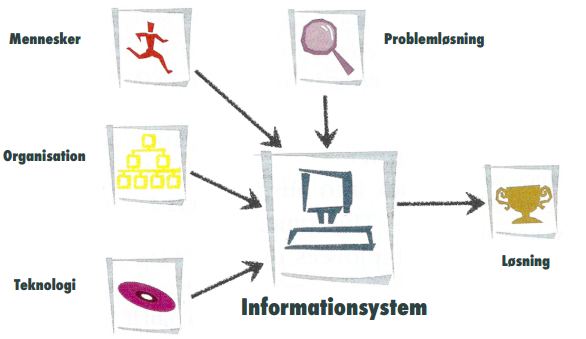
\includegraphics{images/kontekstmodel/metode.png}
  \caption[Metode for Kontekstmodellen]{Illustration af elementerne i et informationssystem. Kilde:
  \protect\citet{Laudon1999}}
  \label{fig:kontekstmodel}
\end{figure}


%\section{Informationssystem}\label{Informationssystem}
\subsection{Informationssystem}\label{subsec:Informationssystem}

Et informationssystem bruges til at effektivisere en arbejdsproces og hjælper med at holde fokus, så arbejdet
bliver gjort tilfredsstillende. Informationssystemet består af tre processor: Indsamling af data, behandling
af dataene og formidling af dataene. Der indsamles data om de tre elementer: mennesker, organisation og
teknologi. Når dataene er indsamlet, behandles de, altså der bliver analyseret på dataene. Herefter formidles
det i form af, der findes ud af, hvad datene kan bruges til. Behandlingen af de tre elementer bruges til at
finde ud af, hvad der skal tages hensyn til under problemløsningsdelen. Alt dette er et informationssystem,
som bruges til finde ud af, hvad løsningen til problemstillingen er.


%\subsection{Mennesker}\label{subsec:mennesker}
\subsubsection{Mennesker}\label{subsubsec:mennesker}

Elementet mennesker handler om personer/persongrupper, som har en interesse i, at en given problemstilling
løses. Det kan være brugeren af det program, der bliver lavet og andre, som får gavn af en løsning. Man
undersøger bl.a. brugerens evner, da programmet skal laves på en sådan måde, at brugeren har den
fornødne kunnen, til at kunne betjene programmet. Brugerens behov undersøges også, så man får alle de funktioner
med, som er nødvendige for at programmet er brugbart.


%\subsection{Organisation}\label{subsec:organisation}
\subsubsection{Organisation}\label{subsubsec:organisation}

Under organisationsafsnittet undersøges hvor og hvordan problemet opstår, derudover undersøges der hvilke regler
og værdier organisationen har, for at kunne tage disse med til problemløsningen.

\cbstart
%\subsection{Teknologi}\label{subsec:Teknologi}
\subsubsection{Teknologi}\label{subsubsec:Teknologi}

Teknologidelen omhandler de teknologier, som anvendes til at løse en informationssystem relevant problemstilling.
Ofte ville denne teknologi være en computere, servere, og internettet. Dette er altså de byggeblokke hvorpå
systemet bygges.
\cbend

%Teknologielementet handler om teknologier som allerede er på markedet, som kan løse problemstillingen. Dette
%behøver ikke kun at være løsninger som er computerbaserede, det kan også være manuelle systemer, altså hvor
%det hele gøres i hånden, med papir og blyant.


%\section{Rapportens opbygning}\label{sec:rapportens-opbygning}
\subsection{Rapportens opbygning}\label{subsec:rapportens-opbygning}

Først bliver menneskedelen behandlet, i form af en interessentanalyse, herefter vil organisationselementet blive berørt. Derefter bliver der skrevet om teknologier,
hvorefter de tre elementer munder ud i en problemafgrænsning og en problemformulering. Til sidst skrives der
om problemløsningsdelen. \fxnote{Sidste sætning skal udvides så der står hvad der vil blive skrevet om}


\part{Problemanalyse}
\chapter{Interessenter for en sejlklub}\label{chap:interessent-analyse-ved-sejlklubber}

I denne interessentanalyse, ses der på mennesker og grupper der har interesse i en specifik software løsning, konkret
til sejlklubber med sejlerskole. Der vil herudover blive set på hvad deres interesse er i projektet, samt hvilken
indflydelse en løsning ville kunne have på deres tilværelse.


Der vil for interessenternes vedkommende blive set på hvad, de hver især kunne få gavn af i henhold til projektet. 
Det er værd at notere at hver enkelte klub har forskellige behov, så dette er en generel forståelse af interessenternes
behov. Forståelsen for de forskellige grupper interessenter er dannet ud fra et Interview med tidligere skolechef på
Sundet. Interviewet kan findes i \myref{bilag:interview}.

\section{Interessenter for sejlklubbers administrative opgaver}

\subsection{Dansk sejlunion}

Dansk sejlunion er et forbund, som blev dannet i 1913, og har ikke nogen direkte grund til at være interesserede i
projektet.
Et af deres mål er som forbund at hjælpe sejlklubber med service, rådgivning mm. og derfor, menes det at Dansk sejlunion
også vil være interesseret i et system der vil kunne hjælpe de frivillige i deres arbejde.

Deres mission er at være det nationale samlingspunkt for alle sejlere. Dansk sejlunion er tilsluttet Danmarks
Idrætsforbund, International Sailing Federation og andre lignende organisationer inden for sejlsport.
\citep{Sejlsportdk}


\subsection{Medlemmer}

Hver sejlklub bestemmer selv deres opbygning organisatorisk af hvilke type medlemmer de har i klubben. Der vil blive
fortalt mere om dette i \myref{chap:organisation}. 

Medlemmerne i sejlklubben er de personer som bruger sejlklubbens faciliteter. Herudover også her klubben får deres
indtægter til at kunne holde sig i gang, og investere i eventuelt nye både el. \fxnote{Sidste sætning skal rettes men
kan ikke gennemskue hvad der rigtigt skal stå?} Det er derfor vigtigt at klubberne gør medlemmernes tid ved sejlklubben
så god som mulig. Et system der kunne hjælpe medlemmerne med at finde informationer, leje både, og som har
medlemmernes interesse i højsædet, vil helt klart kunne være i deres interesse. De førnævnte funktioner i et system til
en sejlklub, er netop funktioner der sandsynligvis ville blive brugt mest af medlemmer.

Medlemmer i en sejlklub kan være en meget bred gruppe fra den yngre befolkningsgruppe, til den noget ældre. Det er
derfor vigtigt at lave et design, som er intuitivt i anvendelse, for alle brugere. 

%Interessentgruppen ``medlemmer'' omhandler medlemmer af sejlklubber. Det er meget forskelligt fra sejlklub til
%sejlklub hvordan medlemmer kategoriseres eller om de overhovedet gøres dette. F.eks. så har ``Sejlklubben
%Sundet'' kategoriseret deres medlemmer således: Voksen-, Bådejer-, Gaste-, Mini-kølbåd-, Ungdoms-, Passiv- og
%Støttemedlem.
%[http://www.sundet.dk/vedtaegter/Vedtaegter%20for%20Sundet%2027nov12.pdf]

%Til sammenligning har Vestre Baadelaug kategoriseret deres medlemmer efter følgende: Aktive-, passive- og
%æresmedlemmer.
%[http://www.aalborglystbaadehavn.dk/UserFiles/file/VB_filer/Statiske_filer/Vedtaegter_2008-9_web.pdf].

%Fælles for medlemmerne er, at de gerne vil have informationer fra klubberne, så de ved hvilke begivenheder der finder
%%sted. Det kan være kapsejladser, foredrag, o.lign. Der er mange informationer, medlemmer fra en sejlklub kan modtage.
%\section{Gæster}:
%Gæster har ikke nogen primær funktion når det kommer til udlån, de bådklubber der tilbyder udlejning af både,
%%forbeholder denne funktion til medlemmer, som har bestået et førerkursus accepteret af den givne bådklub.


\subsection{Undervisere}

En sejlklub med sejlerskole, skal også have undervisere til sejlerskolen, og disse kan også drage nytte af et system til
at hjælpe med administrative opgaver. Underviserne vil ved hjælp af et system eventuelt kunne sende afbuds e-mails eller sms-beskeder ud til alle på
undervisningsholdet. Det vil muligvis kunne gøre det lettere for underviseren at holde styr på den enkelte elevs fremgang
ved undervisningen m.m. hvilket medfører at underviserne bør have andre funktioner i et system til en sejlklub end medlemmerne
ville have, de ville eventuelt kunne stå for at registrere hvem der har et førerbevis i klubben, ol. Underviserne kan også
være frivillige i sejlklubben, men de er beskrevet for sig selv da de har mere specifikke funktioner i sejlklubben. 
Det antages at hvis et system ville kunne hjælpe undervisere med deres opgaver, så de bruger mere af deres arbejdstid på
at undervise, ville det give en positiv respons.

\subsection{De frivillige i sejlklubben}

Der er udover undervisere i en sejlklub også andre frivillige der arbejder i sejlklubben. Dette kan være lige fra en
formand til en sekretær eller måske endda nogen som gør rent i sejlklubben. Disse frivillige kan alle have forskellig
gavn af et system, der kan håndtere deres anliggender i sejlklubben, og er derfor taget med som interessenter. Nogle af
dem kan have til opgave at holde styr på ind- og udbetalinger for medlemmerne, hvilket et medlemssystem ville kunne
hjælpe med. En sekretær ville kunne give nyheder eller referater videre til klubbens medlemmer igennem sådan et
system. Så der er altså mange forskellige muligheder et administrativt system ved en sejlklub ville kunne hjælpe med, og
herudover også mange mennesker der ville kunne få gavn af en løsning.


Disse 4 interessenter, har hver deres interesse for projektet, hvor underviserne og de andre frivillige smelter en smule
sammen. Underviserne samt de andre frivillige, vil gerne have det gjort lettere at udføre deres frivillige arbejde.
Medlemmerne vil gerne have informationer fra klubberne angående begivenheder der
måtte foregå, samt muligheder for at deltage i disse, eller leje sejlbåde.
Dansk Sejlunion er altså en mindre direkte interessent, men kan dog have interesse i at hjælpe nye eller mindre
sejlklubber med at istandsætte et godt administrativt netværk, for at danne en velfungerende sejlklub, 
der giver gode oplevelser for medlemmerne.


\chapter{Organisation}\label{chap:organisation}

\cbstart

\section{Sejlklubben Sundet}

I Sejlklubben Sundet findes flere både, af forskellig størrelse, som bruges til undervisning af klubbens
elever, såvel som udlån til klubbens medlemmer.

Undervisningen foregår hen over hverdagene, hvorimod bådudlån foregår i weekenderne. En enkelt klasse af både
kan dog også udlånes om onsdagen.

For at måtte sejle skal der være minimum én fører med i bådens besætning \fxnote{Husk at definere fører og
muligvis besætning, hvis dette bibeholdes.}. Desuden bestemmes prisen for udlånet bl.a. efter besætning også,
idet tilstedeværelsen af en af klubbens elever gør, at udlånet er gratis.

Håndteringen af de forskellige data blev, og bliver muligvis stadig, udført på papir, ved manuelt arbejde,
hvilket ifølge oplysninger \fxnote{Muligvis angive en mere officiel kilde her?} kan resultere i, at det kun
bliver gjort engang imellem.

Ved et kig på Sejlklubben Sundets hjemmeside \citep{SundetUdlaan} ses det, at forskellige værktøjer er taget i
brug, i et forsøg på at øge brugervenlighed og interaktion mellem deltagere. Det er på nuværende tidspunkt
uvist, hvor vidt disse tiltag har haft den ønskede, gavnlige effekt.

\cbend

\chapter{Teknologianalyse}\label{chap:teknologi-analyse}

I det følgende kapitel vil forskellige teknologier, som kunne anvendes i forhold til at hjælpe med
administrationen i en sejlklub, blive forklaret. Derefter findes en analyse af de programmer, som på nuværende
tidspunkt er state of the art inden for administration af sejlklubber.

\section{Teknologier}

\subsection{Internet}

En fordel for et system til administration i alle typer af klubber og organisationer ville være at kunne tilgå
det fra flere steder end bare et sted. Ved at gøre et system netværksbaseret kunne medlemmer og frivillige
tilgå det fra hjemmet, deres arbejdspladser eller måske endda deres mobile enheder, og derved ville en tur ned
til klubhuset, f.eks. for at undersøge om der var en båd ledig den kommende uge, undgås, hvilket der i
\myref{sec:organisation-konklusion} blev fremlagt som et problem. Anvendelsen af et system, som kunne operere
over internettet, kunne altså øge informationsspredning i klubben. Herved gøre det muligt at lave papirarbejde, som
udfyldelse af log-filer hjemmefra i stedet for i klubben og tilmelde sig sejladser og andre arrangementer
hjemmefra.


\subsection{Server}

For at alle medlemmer og frivillige arbejdere i en klub kan tilgå systemet over internettet, skal systemet
opretholdes af en server, hvorfra andre computere kan forbinde sig til og bruge systemet. En mulighed for
opsætning af en server ville være at få en computer i selve klubhuset til at agere server og have systemet, og
al information, til at ligge der. Dette er dog en dårlig løsning, da klubben selv skulle stå for opdatering af
serversoftware, tage backup af al data og det ville kræve mere af klubbens internetforbindelse. En anden
mulighed for at en klub ikke selv skulle stå med at administrere en server, er at købe sig ind hos et hosting
firma. Her kan man have systemet kørende på en server, og firmaet varetager samtidigt al vedligeholdelse af
server og serversoftware og sørger for backup af al data. Dog kan forskellige firmaer have forskellige måder
at gøre tingene på, men de firmaer der kigges på i de følgende afsnit, \textit{abakomp} og \textit{Softcom}, sørger begge for vedligholdelse og overvågning af serverne, og for at tage backup. 

De typer af servere, der bliver udbudt af hosting firmaer, kan deles op i dedikerede servere og i virtuelle
servere.


\subsubsection{Dedikerede servere}

Ved en dedikeret server lejer man hele maskinen, som skal køre systemet, og man får derfor mere ud af maskinen
og har mere indflydelse på komponenterne i maskinen og hvilket operativsystem der køres. En dedikeret server
ville umiddelbart være bedre for større klubber/organisationer, hvor mængden af informationer serveren skulle
kunne håndtere er større og trafikken til serveren også ville være højere. \citep{Dedikeretserver}


\subsubsection{Virtuelle servere}

Alternativet til at leje en hel maskine til at køre et system, er at leje en virtuel server, hvor der på den
samme fysiske maskine findes flere separate virtuelle servere. At leje en virtuel serverplads er billigere end
at leje en dedikeret server, da en virtuel serverplads kan lejes for helt ned til 850 kr. i
måneden\citep{Virtuelserver}, hvorimod en dedikeret server kan lejes fra 1062 kr. i måneden
\citep{Dedikeretserver}. 
Dog variere prisen alt efter hvilket hardware der bruges og efter, hvor meget
serverplads man ønsker. Grunden til at en virtuel serverplads er billigere, er at flere forskellige virtuelle
servere kan køre på samme fysiske maskine, og derved er der flere til at betale for vedligeholdelsen. Men en
virtuel server har til gengæld ikke lige så meget plads og kraft som en dedikeret server.

En virtuel serverplads ville umiddelbart være nok til at køre et administrativt system for en sejlklub, og det
ville desuden være billigt at leje plads hos et hosting firma. Det er derfor fornuftigt at antage at
sejlklubber har midler til at leje en serverplads, hvilket ville kunne anvendes til at køre et administrativt
system med alle informationer, som kunne være nødvendigt for systemet.


\subsection{Brugergrænseflade}

I et program som skal anvendes af en bruger eller brugergruppe, ønskes det, at programmet har et udseende, som
brugeren forstår og som hjælper med at bruge programmet. Her menes der programmets interface, på dansk,
brugergrænsefladen. Det er vigtigt, at brugergrænsefladen henvender sig til modtagergruppen, hvilket i dette
projekt er personer med tilknytning til en sejlklub. Der skal desuden tages højde for de forskelle i teknisk
snilde, der er i modtagergruppen, da det ikke er effektivt at lave et system, som halvdelen af modtagerne ikke
kan bruge. Forskellige undergrupper i modtagergruppen skal bruge forskellige funktioner i systemet, og derfor
skal interfacet tilpasses, så de korrekte funktioner bliver tilgængelige for de rigtige brugere.

En mulighed for at skabe en brugergrænseflade i samarbejde med C\#-kode, er ved at anvende \textit{Windows
Forms}. Det findes også andre muligheder for at anvende C\#-kode til at skabe brugergrænseflader som
\ac{MVC} og \ac{WPF}, men i løsningsdelen vil
\textit{Windows Forms} blive anvendt til at skabe en brugergrænseflade.

\subsection{Management systemer}\label{subsec:management-systemer}

Et system som med fordel kunne anvendes til det formål, er et management system. Et management system er et
framework af processer og procedurer, som bruges til administration af frivillige organisationer og
virksomheder. Eksempler på management systemer findes i \myref{chap:teknologi-analyse}. Mere præcist er
SailingClubManager et management system, hvilket er yderligere dokumenteret i \myref{bilag:scm}. Det
management system har en \ac{GUI} i web browseren. Dette er i kontrast til en konsol
applikation, eller en nativ \ac{GUI}.

Ved at anvende et management system kan en klub eller forening, forudsat at systemet er succesfuldt, mindske den
tid, der bruges på papirarbejde. Særligt fordi en lang række idrætsforeninger drives af frivillige. Ifølge
\citet{Frivilligrapporten} er 26\% af de arbejdsopgaver, som findes for frivillige, sekretariatsarbejde og
administrativt arbejde. Med et godt management system kan de administrative opgaver derved bringes ned på
mindre tid, og derved kan de frivillige bruge deres tid på mere interessante ting for organisationen, eller
bruge den ekstra tid på noget andet.


\section{State of the art}

For at kunne udvikle et godt produkt, der skal kunne bruges i en bådklub, er det vigtigt, at se på hvilke
produkter der allerede er på markedet, altså hvad er ``state of the art''. I denne forbindelse er der fundet
forskellige produkter, som har nogle af de features der efterspørges i et system til en bådklub.


\subsection*{BoatCloud}

Der er f.eks. et program udviklet af Anderson Software, der hedder BoatCloud.\citep{BoatCloud} BoatCloud
består af 3 applikationer, StackTrack, VesselValet og Service Request. StackTrack benyttes, når medlemmerne selv sejler
deres både, hvorimod VesselValet, er
når der skal tjenere og passagerer med ombord på bådene. BoatCloud applikationerne er derfor mere designet til
en bådklub, som passer på medlemmernes både, fremfor klubbens egne både. I applikationerne kan medlemmerne
melde, at de vil sejle på et bestemt tidspunkt. Medlemmet kan få klubben til at vaske båden, tanke den, og
fylde den op med diverse snacks, alt sammen registreres igennem denne webbaserede applikation. Applikationen
tager imod alle disse bestillinger i realtime, og 24 timer i døgnet. Herudover bliver der sendt e-mails ud til
medlemmerne, når de har lavet en bestilling. Man kan logge ind som administrator, og her kan man se alle
reservationer, der er lavet, samt have mulighed for at se yderligere detaljer om hver enkelt reservation.


\subsection*{Sailing Club Manager}

En anden applikation der findes er Sailing Club Manager \citep{SailClub}. Denne applikation er også
webbaseret, og gør det muligt for en bådklub at tilføje hvilke både der er, samt hvor det er fortøjet i
havnen. Man kan i en kalender lave begivenheder og reservationer, samt medlemstilmeldelse til forskellige
begivenheder. Applikationen kan også bruges som kontaktmedium for klubben til deres medlemmer. Klubben kan
sætte et e-mail system op, samt tilføje et template som bliver sendt med hver enkelt e-mail. Applikationen kan
endvidere holde styr på økonomien, man kan tilføje en bankkonto, samt  holde styr på fakturaer, og endda sende
dem og håndtere det online. Man kan tilføje medlemsskaber, med forskellige oplysninger omkring medlemmerne der
har netop dette medlemsskab i klubben.



Ud fra denne undersøgelse er flg. features altså fundet i applikationerne:

\begin{itemize}
  \item Medlemmer kan reservere afgange
  \item Medlemmer kan melde sig på begivenheder i bådklubben
  \item Medlemmer kan betale igennem hjemmesiden
  \item Medlemmerne kan bede klubben om at gøre deres egen båd klar, med forskellige aftaler klubben håndterer
        før den aftalte tid
  \item Bådklubben kan vise hvilke både der er i klubben
  \item Bådklubben kan oprette begivenheder, og afsætte hvilke medlemmer der kan melde sig på begivenheden
  \item Bådklubben kan oprette forskellige medlemsskaber og opkræve betalinger igennem hjemmesiden
  \item Bådklubben kan sende e-mails med klubbens egen template gennem hjemmesiden, herunder påmindelser om en
        reservation nogen tid før.
\end{itemize}

I bilag \myref{bilag:scm} findes der screenshots af udvalgte features der findes i SailingClubManger.

\subsection*{ForeningLet}

ForeningLet er en applikation, som adskiller sig fra de andre ved ikke at henvende sig specifikt til én type klub, desuden er det en dansk applikation. Applikationen er web-baseret og har mange nyttige funktioner for en sejlklub som Sundet. Applikationen har en medlemsdatabase, et regnskabssystem samt en kontaktfunktion som kan benytte både e-mail og SMS. Der kan også opkræves betalinger fra medlemmerne gennem systemet. Applikationen har også en reservationsfunktioner. Desuden kan der oprettes begivenheder i applikationen, som medlemmerne også kan tilmelde sig gennem applikationen. ForeningLet giver også foreningen mulighed for at oprette deres egen hjemmeside samt deres egen online butik. 


\section{Konklusion af teknologianalyse}

Ud fra teknologianalysen er de teknologiske aspekter i projektet blevet belyst. Muligheden for at gøre
systemet netværksbaseret, gør det muligt for medlemmerne og administrationen i en sejlklub, at foretage
handlinger vedrørende klubben fra hjemmet eller arbejdspladsen. For at undgå at en lokal server skulle
opsættes og vedligeholdes af klubben selv, kunne en virtuel server, hostet af et hosting firma, varetage denne
opgave. Vigtigheden i en god brugergrænseflade blev gjort klart, og metode for at opsætte en brugergrænseflade
blev valgt i form af \textit{Windows forms}. Fra state of the art delen blev nuværende systemer på markedet
undersøgt, og udvalgte features tages med videre til løsningsdelen, som eventuelle tilføjelser til det
administrationssystem der skal udvikles.



\chapter{Problemformulering}\label{chap:problemformulering-new}

Indtil nu er problemet om fritidsklubbers administrative opgaver blevet belyst og analyseret vha. Laudon og Laudons model beskrevet i \myref{chap:struktur-af-problemanalyse}. 
Det er nu ud fra denne analyse muligt at komme frem til en problemformulering, som der vil arbejdes ud fra i løsningsdelen henimod en løsning til fritidsklubber og ikke mindst sejlklubber.

Der blev i \myref{chap:Fritidsklubber}, omhandlende fritidsklubber, afgrænset til sejlklubber, da disse viste sig at have flere specifikke administrative opgaver, sammenlignet med andre fritidsklubber. 
Denne afgrænsning blev foretaget da et system, der kan håndtere generelle samt specifikke opgaver til en sejlklub, kan bruges af andre former for fritidsklubber ved at tilpasse specifikke funktioner.
Ved at analysere videre på de direkte forhold vedrørende en sejlklub, blev der dannet en forståelse for, hvilke problemer en sejlklub med sejlerskole har, som kan løses vha. et administrations system.


\section{Interessenterne for sejlklubber}

Der var forskellige interessenter for sejlklubberne, og de havde varierende mængder af interesse i projektet.

Medlemmerne, underviserne og de frivillige vil alle være personer der skal bruge det udviklede system. 
De har derfor en mere direkte indvirkning på, hvordan system skal opbygges. 
Hvis systemet ikke har de funktioner, som de efterspørger, vil det ikke være den gode løsning, som de gerne vil have. 
Dette gælder for alle de tre nævnte interessenter. 
Det skal dog understreges, at de ikke vil bruge samme dele af systemet. 
Dette skyldes, at medlemmerne ikke skal kunne oprette undervisningsdage mm., da det kun er underviserne, der skal have tilladelse til dette. 

\section{Organisation}

I forbindelse med organisationsafsnittet blev der undersøgt, hvordan sejlklubberne håndterer forskellige opgaver i klubben, samt hvilke opgaver de beskæftiger sig med.

Det viste sig, at klubberne har individuelle medlemstyper, og det kan derfor være relevant at lade klubberne selv oprette forskellige medlemstyper i systemet. 
Desuden efterspørges det, at man kan tilkoble sig systemet hjemmefra, for således at kunne få informationer om begivenheder og undervisning i klubben, og måske endda tilmelde sig disse, uden at tage turen ned til klubben.

Grundet den store mængde af information, der skal nedskrives, i forbindelse med en sejlads, giver det mening at hjælpe med at organisere denne opgave, samt at gøre det lettere at registrere informationerne for diverse frivillige og undervisere. 
Desuden kunne det hjælpe hvis hvert medlem havde en saldo over udgifter ved sejlklubben, således det er nemmere at håndtere brugerbetaling.

Følgende er en liste over opgaver, som kan dækkes af et system for sejlklubberne:

\begin{itemize}
  \item Tilkobling hjemmefra, via internettet
  \item Mulighed for at få informationer vedr. begivenheder, samt at tilmelde sig disse
  \item Organisering af information der nedskrives i forbindelse med en sejlads
  \item Organisering af betalinger, samlet for det enkelte medlem, samt mulighed for online betaling
  \item Booking af både
  \item Administrering af undervisning
\end{itemize}


\section{Teknologi}

Sejlklubben Sundet, viste sig at have flere forhold at organisere end de andre klubber der er undersøgt, og derfor afgrænses projektet til konkret at designe et IT-system til Sundet. 
Dette gøres da hvis et system kan hjælpe Sundet, er det blevet konkluderet, at det også kan hjælpe andre sejlklubber, der har færre forhold at holde styr på.
Man har fundet frem til at systemet, der efterspørges, er af typen management system, som blev beskrevet i \myref{subsec:management-systemer}.
Der findes allerede systemer, som kan dække Sundets administrative behov, bortset fra håndteringen af undervisning.
Der mangler altså et program på markedet, som kan håndtere en sejlklubs sejlerskole.
Heri ligger projektets eksistensberettigelse.

\subsection*{Problemformulering}
\subsubsection*{Ud fra denne afgrænsning er flg. problemformulering formuleret:}

\begin{center}
  \begin{tabular}{|p{14cm}|}
    \textit{Det er et problem at frivillige i fritidsklubber med specielle udlejningsmuligheder, så som Sundet, benytter unødvendig arbejdskraft på fysisk dokumenthåndtering vedrørende udlånte faciliteter, undervisning og begivenhedsorganisation. 
    Hvordan kan et system hjælpe med at danne overblik over sådanne opgaver?}
  \end{tabular}
\end{center}
\fxnote{Nikolaj: bør det ikke nærmere være: "Hvordan kan der udvikles et system som kan hjælpe med at danne overblik over sådanne opgaver?}


\section{Afgrænsning for problemløsning}

Da dette projekt er udarbejdet i løbet af 2. semester på Aalborg Universitet, er der ikke uanede mængder af tid. 
Der afgrænses derfor fra at udvikle hele management systemet til sejlklubben Sundet, til i stedet at lave enkelte dele af systemet.

Grundet de manglende ressourcer og tid, vil der altså ikke blive lavet et system, der kører over internettet, men i stedet et system, som kan håndtere de forskellige emner lokalt. 
Denne afgrænsning finder sted, da hvis funktionerne for klubben kan fungerer på computeren, skal det tilkobles en server, for at kunne tilgåes fra flere forskellige computere. \fxnote{Hvad menes der med ``computeren'' er det den nede i klubben, eller enhver?}
Derfor ser projektgruppen altså funktionerne for Sejlklubben Sundet som værende de vigtige ting at udvikle, selvom systemet mister noget af sin effektivitet uden internetopkoblingen.\fxnote{Nikolaj: Omformulering: " selvom systemet mister sin brugbarhed uden internetopkoblingen}
Men dette ses som værende acceptabelt, da systemet ikke skal tages i brug af klubben, da dette er et projekt lavet i forbindelse med uddannelsen på Softwareingeniørstudiet ved Aalborg Universitet.

De resterende kapitler i rapporten, vil beskæftige sig med udviklingen af et management system, henvendt imod Sejlklubben Sundet, baseret på problemformuleringen. 
Som det første vil der komme en kravspecifikation for systemet, på baggrund af denne afgrænsning.



%\part{Problemløsning}
%\chapter{Eksempler}

{\itshape Dette dokument er primært ment som en hjælp til at se de forskellige muligheder
i rapporten.}

\section{Akronymer}
For lettere at håndtere akronymer, benyttes en pakke, hvor disse defineres én gang, og bruges så i
dokumentet ved hjælp af \textbackslash ac{acronym}. Så vil systemet sørge for, at skrive det fuldt
ud første gang man eksempelvis skriver \ac{AAU} eller \ac{KOT}.

Skulle det derefter ske, at man har behov for at snakke om \ac{AAU} igen, vil den bruge forkortelsen,
og dermed selv holde styr på det. Dette sikrer os bedre mod fejl. :)

\section{Ændringsregistreringer}
For at lette kommunikation med vejleder kan vi registrere ændringer på forskellige måder.

\subsection{Hele afsnit}
\cbstart Man kan markere, at et helt afsnit er blevet ændret eller tilføjet, ved hjælp af kommandoerne
\textbackslash cbstart og \textbackslash cbend, som markerer henholdsvist start og slut på sidebaren.\cbend

Det er også muligt at markere, at noget er blevet slettet, med \textbackslash cbdelete, hvilket er gjort i
dette \cbdelete afsnit.

\subsection{Detaljerede ændringer}
Der er også mulighed for at vise mere detaljerede ændringer. Eksempelvis \added[id=TB]{hvis man tilføjer tekst},
eller \deleted[id=TB]{sletter tekst}. Eller for den sags skyld \replaced[id=TB]{en kombination af de to}{a
combination of the two}.

\section{Matematik}
Matematiske formler er lette at indsætte\ldots

\begin{equation} \label{eq:example}
  f\left(x\right) = \dfrac{a \cdot b}{c}
\end{equation}

\section{ToDo--typer}
Der er fire forskellige typer af noter, og brugen heraf bestemmes af gruppen i fællesskab, så der er enighed om,
hvad der benyttes til hvilket.

\subsection{Generelt}
Først og fremmest er der noterne almindelig\fxnote{Peger på et bestemt sted i teksten.}
og \fxnote*{Fremhæver et tekststykke også.}{med modtagertekst}.

Ligeledes er der advarsler\fxwarning{Dette er en advarsel!} og fejl\fxerror{Dette er en fejl!}. Sidstnævnte
vil desuden forhindre dokumentet i at kompilere, hvis det markeres som værende \emph{final}.

Disse tre typer kan naturligvis også bruges i \emph{stjerneformen}, til at fremhæve et bestemt stykke
tekst som denne tilknyttes.

\subsection{Avanceret}
Til de lidt mere krævende noter kan det være nødvendigt med mere tekst, hvilket kræver et environment.

\begin{anfxnote}{Dette er en opsummering.}
Dette kan benyttes til at få nogle længere noter ind i teksten, hvis der eksempelvis er noget der skal
overvejes, hvor det bare ikke er nok men en lille notits.

Foruden denne anfxnote er der også \emph{anfxwarning}, \emph{anfxerror} og \emph{anfxfatal}, ligesom ovenfor.
\end{anfxnote}


\section{Referencer}
Det er muligt at referere til forskellige ting, eksempelvis kan nævnes \myref{eq:example}.

For at oprette en såkaldt \emph{label}, som senere kan refereres til, benyttes \verb|\label{key}|. Det er god
stil indenfor \LaTeX at benytte prefixes til de forskellige labels, eksempelvis:
\begin{table}[h]
  \begin{center}
    \begin{tabular}{ll}
      \toprule[1.5pt]
      \texttt{chap:}   & chapter              \\ 
      \texttt{sec:}    & section              \\ 
      \texttt{subsec:} & subsection           \\ 
      \texttt{fig:}    & figure               \\ 
      \texttt{tab:}    & table                \\ 
      \texttt{eq:}     & equation             \\ 
      \texttt{lst:}    & code listing         \\ 
      \texttt{itm:}    & enumerated list item \\ 
      \texttt{ex:}     & example              \\
      \bottomrule[1.5pt]
    \end{tabular}
  \end{center}
  \caption{Reference prefixes} \label{tab:reference_prefixes}
\end{table}


\section{Eksempelbokse}

\begin{example}{Overskrift}
  \label{ex:an_example}
  \lipsum[1]
\end{example}



\section{Programmeringskode}



\makeatletter\@openrightfalse
\let\cleardoublepage\clearpage
\part{Problemløsning}
\chapter{User stories}\label{User_stories}
Til definering af de funktioner programmet skal indeholde, er der blevet brugt user stories.\fxnote{Nikolaj: "definering"!? "udarbejdelse" måske?}
Ud fra disse user stories er det nemt at danne egentlige kravspecifikationer for programmet. \fxnote{Troels: ``er det nemt'' ?? bare skrive dannes}
Under udviklingen kan det også bruges som en checkliste, så der ikke glemmes funktionaliteter. 

\section{Medlemmer}
Som en \textbf{bruger} kan jeg se sejlklubbens kalender.
\newline
Som en \textbf{bruger} kan jeg ændre eller slette mine reservationer, hvis jeg ombestemmer mig.
\newline
Som en \textbf{bruger} kan jeg se hvor mange ture jeg har taget, så jeg kan se hvor meget jeg skal betale.\fxnote{Nikolaj: Dette er ikke opfyldt, bør der så ikke skrives om hvorfor den ikke er det et eller andet sted?}
\newline
Som en \textbf{bruger} vil jeg kunne logge ind i programmet.
\newline
Som en \textbf{bruger} vil jeg have en 'mine oplysninger' type side. \fxnote{Troels: Vær mere specifik?}
\newline
Som en \textbf{bruger} vil jeg gerne kunne se hvilke andre medlemmer der er i sejlklubben, for at kunne aftale fælles sejlture med dem.
\newline
Som en \textbf{administrator} vil jeg gerne være i stand til at se detaljeret information om de medlemmer, der er i sejlklubben.
\newline
Som en \textbf{administrator} kan jeg importere medlemmer fra andre systemer, så de kan blive genbrugt.
\newline
Som en \textbf{administrator} vil jeg have en speciel administratordel af programmet.
\newline
Som en \textbf{administrator} vil jeg kunne angive rettighedsniveau for medlemmerne.

\section{Både}

Som en \textbf{bruger} kan jeg se informationer omkring bådene, så jeg kan vurdere hvilke jeg kan sejle. \fxnote{Troels: Dette er ikke opfyldt? Skal vi redegøre for hvad der er og ikke er opfyldt senere på en mere konkret måde? evt i diskussion}

\section{Bådudlån}

Som en \textbf{bruger} kan jeg reservere både.
\newline
Som en \textbf{administrator} kan jeg se hvor mange ture hver bruger har taget, så jeg kan kræve det korrekte beløb fra dem.

\section{Undervisning}
Som en \textbf{bruger} kan jeg se informationer omkring sejlerskolen, så jeg kan følge mine fremskridt, se fremtidige lektioner osv. \fxnote{Troels: Her menes vel som elev?}
\newline
Som en \textbf{elev} vil jeg kunne se hvilke lektioner jeg har været til og hvilke jeg ikke har, samt melde afbud til kommende lektioner.
\newline
Som en \textbf{elev} vil jeg være i stand til at tilmelde mig lektioner også andre end på det hold jeg normalt er på.\fxnote{Nikolaj: Dette er heller ikke opfyldt}
\newline
Som en \textbf{underviser} vil jeg gerne være i stand til at kontakte de elever, som er med i sejlerskolen.
\newline
Som en \textbf{underviser} kan jeg se og ændre brugers fremskridt i sejlerskolen, så brugerne bliver opdateret.
\newline
Som en \textbf{underviser} vil jeg kunne se en liste over mine elever.
\newline
Som en \textbf{underviser} vil jeg have en oversigt over mine lektioner samt deltagere til disse.

\section{Begivenheder}
Som en \textbf{bruger} vil jeg kunne se hvilke begivenheder der er i klubben, samt melde mig til dem.

\fxnote{Troels: Som admin lav behivenheder?}
\chapter{Produktkrav}

Igennem problemanalysen blev det gjort klart, at der findes et problem ved fritidsklubber, særligt Sejlklubben Sundet, når det kommer til management af deres ressourcer samt dokumenthåndtering. 
Problemet kan løses ved et management system, til at håndtere dokumentation for sejlklubben og gøre det overskueligt. 
I følgende afsnit undersøges der, hvilke krav et managements system for Sejlklubben Sundet skal have. 


\section{Funktionelle krav} \label{sec:funktionelleKrav}

Den nødvendige dokumentation indebærer logbøger, bådreservationer, besætningslisten, tilmeldinger til begivenheder m.m. 
Som grundlag for at alt dette kan fungere, kræves der en metode til at sætte sig selv på en aktivitet. 
For at gøre dette muligt kræves der således to ting: En database af medlemmer, samt en form for begivenhedskalender. 
Foruden dette kræves der information om de forskellige begivenheder og hvem der er tilmeldt. 
Der kræves også et system til udlejning af både samt undervisning.

Produktet bør have følgende funktioner i prioriteret rækkefølge:
\begin{itemize}
  \item Medlemshåndtering
  \item Brugerlogin
  \item Oversigt over undervisning
  \item Bådreservation
  \item Logbog
  \item Vise begivenhedsinformation
\end{itemize}


%Dette afsnit skal uddybes meget mere, har skrevet et eksempel på hvad jeg mener afsnittet skal indeholde

\section{Uddybning af funktionelle krav}

Der ligger mere bag de ovenstående elementer end \myref{sec:funktionelleKrav} giver udtryk for, disse vil her blive set nærmere på.

\subsection{Medlemmer}

Det er et krav at man kan udnytte medlemmerne i klubben, så man kan registrere hvem der er tilmeldt de forskellige reservationer eller lignende. 
Systemet skal kunne kende forskel på medlemmer, så man ikke kan have flere af det samme medlem på en reservation eller en begivenhed.
Forskellige informationer skal kunne findes på medlemmerne i programmet, så brugerne kan finde de rigtige medlemmer og markere om de mødte op.

\subsection{Login system}
Det skal være muligt at registrere hvem der er logget ind i programmet, for på denne måde at give forskellig adgang til diverse funktionaliteter i programmet.

\subsection{Oversigt over undervisning}

Det skal være muligt for elever ved sejlerskolen at se hvornår deres næste lektion finder sted.
Herudover skal de også kunne se hvor langt de er kommet i forbindelse med deres uddannelse. Hvilke milepæle de har udført, mm.
Underviserne skal have mulighed for at oprette nye lektioner og angive hvilke læremål eleverne udførte i den pågældende lektion. 
Underviserne skal også kunne udforme og redigere hold på skolen hvis nogle skulle melde sig ud, eller ved sæsonstart.

\subsection{Bådreservation}

Medlemmerne i klubben har muligheden for at reservere klubbens både, og skal derfor kunne gøre dette i programmet.
Derfor skal der være en måde hvorpå man kan tjekke om en båd er booket i en given tidsperiode, og samtidig en måde hvorpå man kan reservere båden.
Herudover skal det være muligt af afmelde sig en booking hvis man ikke deltager alligevel, og dermed åbne op for nye besætningsmedlemmer.


\subsection{Logbog}

I forbindelse med en sejltur, skal der kunne gemmes en logbog over turen med informationer, som beskrevet i \myref{subsec:bådudlån}.
Der skal her være registreret på hvilken både turen foregik, så de korrekte logbøger kan findes for en given bog.

\subsection{Vise begivenhedsinformation}

Endeligt skal man kunne gemme begivenheder i klubben, med en dato og en beskrivelse af begivenheden. 
Det skal være muligt at til- og afmelde sig begivenheden, foruden at kunne se hvilke medlemmer der er tilmeldt.
Desuden skal der kunne vise en liste over begivenheder sorteret efter dato, så man kan danne et overblik over hvornår der sker hvad i klubben.

\chapter{Arbejdsproces}\label{chap:arbejdsproces}

I dette afsnit vil projektets proces for udviklingen af programmet beskrives, som baseres på et begreb kaldet ``agile software development''.

\section{Agile software development}\label{sec:agile-software-development}
Når agile software development benyttes i udviklingsprocessen ligges der fokus på at lave et fungerende program.
Dette anvendes for at holde programmets omfang realistisk, ved tankegangen:
``begynd ikke på noget der ikke er tid til eller kun kan udvikles delvist''.
Med dette menes der, at hver enkelt funktion skal fungere fejlfrit, før arbejdet med den næste påbegyndes. 
Der tilstræbes altså at have et mindre og fejlfrit program, fremfor et større fejlfyldt program.

Agile software development ligger yderligere fokus på ``co-location'', således at arbejde bliver udført på en arbejdsplads med ens kollegaer eller medstuderende, i stedet for at hver person sidder for sig selv, heri ligger ``pair programming''. 
Ved denne metode programmerer to programmører på en enkelt computer, med en fører og en observatør, for øget kodekvalitet.
\fxfatal{Marc, find din kilde}

\section{Faktiske arbejdsproces}\label{sec:faktiske-arbejdsproces}
Pair programming er delvist blevet anvendt i programmeringsprocessen, dvs. at noget af kildekoden er skrevet med denne programmeringsteknik.
Således er mindre dele af kode skrevet af enkeltpersoner, som efterfølgende er gennemgået af andre gruppemedlemmer.
Tankegangen med at en funktionalitet skulle være færdig før der blev startet på ny, blev overholdt i starten af udviklingsprocessen.
Der gik dog ikke lang tid, før der blev fraveget fra dette, da det faldt gruppen svært at opdele de enkelte funktioner i små dele, som kunne laves af forskellige personer eller pair programming grupper.
I stedet for blev arbejdet med andre funktioner påbegyndt, så alle i gruppen havde noget at lave.  

\chapter{Grafisk teori}

\fxnote{Nikolaj: Måske skulle der skrives noget metatekst her?} \fxnote{Marc: Forslag til dette ``I forbindelse med udvikling af en grafisk brugergrænseflade, undersøges ud fra målgruppen retningslinjer til sådan en brugergrænseflade i dette afsnit.''}

\section{Grafisk brugergrænseflade} \label{chap:GUI}

I forbindelsen med udviklingen af systemet, skal man sørge for at designe det, så brugerne kan finde rundt i de forskellige funktioner. \fxnote{Troels: Forslag til ny sætning: ``Centralt for systemets design, er at brugerne kan navigere rundt i det.''}
Da Sejlklubben Sundets medlemmer kan bestå af en mangfoldig gruppe af mennesker, er det svært at indskrænke brugerne i en enkelt gruppe, dermed formodes det at IT-evnerne kan være meget forskellige.


\subsection{Designet} \label{sec:Designet}

Programmets brugergrænseflade vil blive designet ud fra principperne i følge Kang og Kims fortolkning. \citep{gui1} 

\begin{itemize}
	\item Minimalisme
	\item Konsistent\fxnote{Troels: indsæt evt. ``(Fra engelsk: Consistency)'' Marc: eller oversæt blot korrekt fra engelsk?: Overensstemmelse}
\end{itemize}

Minimalisme betyder, at der skal være så få forstyrrelser på skærmbilledet som muligt. 
Det skal være enkelt og simpelt at navigere rundt og finde de funktioner i programmet, man skal bruge. Knapper skal gerne være holdt til et minimum og mindre brugte funktioner gemmes derfor væk i menuer eller andre vinduer.
En sådan struktur skal dog ikke have et hierarki, der er dybere end tre niveauer for ikke at gemme funktioner for brugeren.
Unødvendige ikoner og lange sætninger er således også kun til forvirring for brugeren og skal gerne undgås.
Labels, der forekommer på brugergrænsefladen skal også gerne være konsistente, dette gælder hele brugergrænsefladen, farver, funktionstyper så som tilføj og fjern samt teksttype og størrelse for at undgå forvirring for brugeren.\fxnote{Nikolaj: Lidt uklart hvad der menes med ``tilføj og fjern''}
Således skal den samme navigationsstruktur også være tilbagevendende igennem brugergrænsefladen.

Disse forskellige principper eller retningslinjer, er forsøgt implementeret i systemet.


\subsection{Implementation}\label{sec:Implementation}

Menustrukturen består af tabs, som er store og lette at se.
De forskellige funktioner i programmet er delt op i deres tilhørende tabs, og man kan altid gå ind i en ny tab uanset hvor, man befinder sig i programmet. 
Dette betyder, at strukturen ikke har et hierarki, da uanset hvor man befinder sig, kan der navigeres ind i alle programmets funktioner.\fxnote{Nikolaj: Det kan godt være jeg har misforstået noget, men er der ikke et hieraki når man f.eks. reserverer en båd? Marc: foruden dette så har vi vinduer der benytter sig af ``showdialog'' hvilket således gør at der ikke kan navigeres fra dem til andre tabs}

Når brugergrænsefladen er lavet, skal den dermed også testes. \fxnote{Troels: Det er jo ikke kun brugergrænseinterfladen ;) som skal testes? Men også resten. ``dermed'' lyder lidt dumt?}
Der vil blive forklaret hvordan dette vil blive gjort i \myref{test_af_program}.

\section{Valg af grafikframework} 
\fxnote{Troels: Kort meta tekst? Marc: forslag ``Dette afsnit omhandler enkelte valgmuligheder for udviklingen af programmet, såvel som begrundelse for det valgte framework, WPF''}

\subsection{Windows Presentation Foundation}
\ac{WPF} er en grafisk brugergrænseflade på Windowsbaserede applikationer. \fxnote{Caspar: Det er da ikke WPF der er brugergrænsefladen, men næremere det værktøj man bruger til at skabe det?} 
WPF gør brug af  bl.a. vektorbaseret rendering af grafik, databinding, til nem redigering af data igennem den grafiske brugergrænseflade, og har også inkluderet \ac{XAML}, hvilket er en nem måde at skabe WPF-grafik på. \fxnote{Troels: ``nem'' og er det XAML som gør det nemt? Er det ikke nærmere visual studios interface?}
Selve C\#-koden, den såkaldte Code-Behind, ligger i en separat fil, med samme navn som XAML-filen. 
Hvis der f.eks. er skabt en Button, en almindelig knap, i XAML-filen, så vil det kode, som Button'en skal udføre, blive placeret i Code-Behind-filen, så grafikken og koden bliver hver for sig, hvilket kan give et bedre overblik. \citep{wpf} \fxnote{Troels: Dog er viewer og controller stadig samlet. Hvilket gør det svært at lave et nyt interface uden at skulle copy paste en masse logik -- Marc: Dette er vel vores brug af WPF der har gjort dette og ikke WPF som generel platform og skal derfor ikke nævnes i en beskrivelse af WPF?}

\subsection{Windows Forms}
Windows Forms (WinForms) er, som \ac{WPF}, en grafisk brugergrænseflade på Windowsbaserede applikationer. \fxnote{Troels: på applikationer? til applikationer, eller på windows platformen, Caspar: Igen, er det ikke nærmere værktøjet til at skabe brugergrænsefladen?}
WinForms er forgængeren til WPF, hvilket betyder at WPF har nogle nye features, som WinForms ikke har.
WinForms har ikke XAML, så selve grafikken skal skrives sammen med selve koden. \fxnote{Tristan: Dette lyder lidt misvisende. Så vidt jeg ved gemmer WinForms informationer om, hvordan brugerfladen er opbygget, i en fil ligesom med XAML. Det er bare ikke en fil der er beregnet til at kunne redigeres.}
Hvor WPF er bygget helt fra bunden, så er WinForms et ``lag'' oven på standard Windows API (WinAPI), hvilket betyder, at hvis det man vil lave i WinForms, ikke er en del af WinAPI, så kan man ende med at skulle bruge 3. parts kode, for at kunne lave det i WinForms.\fxnote{Tristan: Eller man kunne programmere komponenterne selv, som programmører har gjort det siden de første grafiske Windows-varianter kom frem.}\citep{winforms2}

\subsection{Website}
En anden mulighed, som blev diskuteret, var at bruge en hjemmeside, som ville have den fordel, at den kan køre på stort set alle enheder, som har adgang til internettet via en browser. 
En hjemmeside, som gør brug af C\#, vil kunne laves på en måde, som minder om den ved WPF og XAML; med HTML (HyperText Markup Language), JS (JavaScript) og CSS (Cascading Style Sheets) som front-end og C\#-klasser som backend. \fxnote{Troels: C\# klasser lyder lidt forkert, måske bare C\# som backend?}

\subsection{Afgrænsning}
En hjemmeside blev fravalgt, da det blev vurderet at WPF var nemmere at oprette end en hjemmeside.
Samtidig bør fokus være rettet mod objektorienterede principper fremfor udvikling af brugergrænseflade. \fxnote{Bør fokus være, eller er vores fokus? (søren)}

WinForms blev fravalgt, da det er ved at være forældet.
Microsoft har informeret om, at der ikke længere tilføjes nye funktioner til WinForms, men at der udelukkende bliver lavet rettelser af fejl.\citep{winforms}

I dette projekt bruges \ac{WPF} til at skabe den grafiske brugergrænseflade. 
Valget faldt på \ac{WPF}, da \ac{XAML}, som WinForms ikke har, gør det let at hurtigt lave en grafisk brugergrænseflade og ligeledes skaber et bedre generelt overblik, når der skabes en brugergrænseflade.\fxnote{Tristan: Igen ``let'' ligefrem? Tror vi bør overveje vort ordvalg.}


\subsection{Ofte anvendte WPF-controls}
I projektet anvendes bestemte WPF controls til at bygge brugergrænsefladen. 
De hyppigst anvendte vil her blive beskrevet. 
På figur \ref{img:wpfdemo} vises de beskrevne elementer (Note: De 3 sidste elementer er henholdsvis DataGrid, ComboBox og ListBox).\fxnote{Nikolaj: Kan billedet ikke laves således, navnet også står i de sidste tre ting?}

\subsubsection*{ComboBox}
I WPF er en ComboBox det element, som andre steder omtales som en dropdown menu. 
Dens indhold kan indstilles enten i XAML-koden eller i Code-Behind koden (her ment C\#-koden).\fxnote{Nikolaj: Muligvis skulle det i parentes, stå første gang Code-Behind bliver nævnt?}
Hvis dette indhold skal være dynamisk, vil Code-Behind ofte være anvendt, eksempelvis hvis man kun vil have de medlemmer af en liste, som opfylder et givent prædikat.\fxnote{Tristan: Skal vi eventuelt nævne, at dette ikke er tilfældet, hvis man benytter sig af binding? (Søren): Kan også abre skrive "Kan man anvende code-behind".}

\subsubsection*{Button}
En Button er en knap, som kalder en metode i Code-Behind koden, når den trykkes på. \fxnote{Kan man ikke bare skrive " I Code-Behind"(Søren)}
Den metode udfører det kode, som er angivet i den.\fxnote{Nikolaj: Sidste sætning bør vel nukes}

\subsubsection*{DataGrid}
Et DataGrid er et grafisk element, som kan vise data dynamisk.\fxnote{Tristan: Måske fremhæve, at der er tale om tabular data? Næsten alle komponenter kan vel vise dynamisk data?}
Ofte vil det vise en liste af objekter.
Dets layout er opdelt i rækker og kolonner, hvor hver kolonne indeholder en bestemt type data, og kan sorteres ved at klikke på de forskellige headers.
Det er også muligt at konstruere en søgefunktion, altså kan et DataGrid blive filtreret.

\begin{wrapfigure}[22]{R}{0.5\textwidth}
    \label{img:wpfdemo}
    \vspace{-30pt}
    \begin{center}
        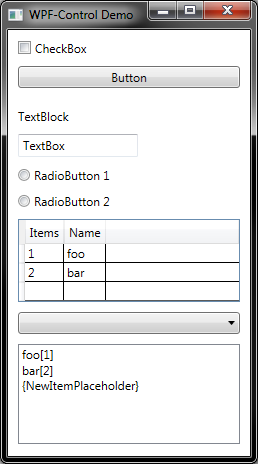
\includegraphics[width=0.48\textwidth]{UI/WPF-Demo.png}
    \end{center}
    \vspace{-15pt}
    \caption{Demonstration af WPFs Controls}
    \vspace{-15pt}
\end{wrapfigure}

\subsubsection*{CheckBox}
En CheckBox er en kvadratisk boks, som enten er ``Checked'' eller ikke-``Checked''.\fxnote{Marc: UnChecked?} 
Ud fra om den er ``Checked'' eller ej, kan der valideres på data. 

\subsubsection*{RadioButton}
En RadioButton er en cirkelformet CheckBox.
Dog vil RadioButtons ofte optræde i serie, altså to eller flere sammen, da valget af den ene ekskluderer valget af de andre. 
Et oplagt brug af dem er til ja, nej (og måske) situationer, hvor kun en af dem skal vælges.

\subsubsection*{TextBlock}
En TextBlock bruges til visning af tekst, som ikke kan redigeres.
Det vil typisk være en forklarende tekst op ad et andet grafisk element.
Det er også muligt at ændre en TextBlock via Code-Behind. 
Hvis man vil føre en dialog med brugeren, eksempelvis til fejlbeskeder.\fxnote{Tristan: Det lyder forkert at starte denne sætning med ``Hvis''. Virker som om der burde komme mere, når man når til punktummet.}

\subsubsection*{TextBox}
En TextBox er et tekstfelt, hvori brugeren kan indtaste tekst. 
Dette kan dermed ses som et inputfelt. 
Det er også muligt at sætte sådan et felt til at være skrivebeskyttet, imens programmet selv kan ændre det.\fxnote{Tristan: Eventuelt ``at være skrivebeskyttet, så brugeren ikke kan redigere det, mens programmet stadig kan foretage ændringer.'', eller noget i den stil?}

\subsubsection*{ListBox}
En ListBox er en tabel, med én kolonne og flere rækker, hvori en bruger kan vælge en eller flere elementer.\fxnote{Nikolaj: Er der tale om en tabel, når der kun er en kolonne. Tristan: Er det ikke bare en liste?}
ListBoxen er i stand til at indeholde samlinger af data på enhver form, oftest vil det være en streng, men et billede er også en mulighed.
Den vil i nogle tilfælde have samme brugsscenarie som en ComboBox eller et DataGrid. 
Forskellen fra en ComboBox er, at der kan være flere synlige elementer i en ListBox på samme tid, samt der ikke er nogen dropdown menu.
Et DataGrid kan indeholde flere informationer på kolonner, mens en ListBox kun kan indeholde én information.\fxnote{Tristan: Dette virker redundant, og måske endda forkert, med den måde det er formuleret på.}

\subsubsection*{UserControls}
Det er muligt at konstruere sine egne grænsefladeelementer fra et eller flere af WPFs indbyggede eller 3. parts Controls.
Dette kaldes en UserControl, som indeholder både en grafisk del og en Code-Behind del.
Det brugerskabte element kan derefter genbruges flere steder i programmet.
Dette er et eksempel på genanvendelse, hvilket kan bidrage til højere programkvalitet og større konsistens gennem programmet. \fxnote{Troels: Tilføj evt. ``UserControls gør et program mere modulært, og gør det nemmere at modificere.'' ?}

\fxnote{Skal vi også beskrive et vindue egentlig ? (Søren)}

\chapter{Programopbygning}

I dette kapitel vil programmets opbygning blive beskrevet. 
Først vil programmets arkitektur blive beskrevet, derefter navigeringen i programmets brugergrænseflade. 


\section{Programopbygning}\label{sec:programopbygning}

\begin{figure}[h]
\centering
\tikzstyle{lille} = [rectangle, minimum width=2cm, minimum height=1.0cm,text centered, draw=black, fill=blue!30]
\tikzstyle{invi} = [draw, rectangle, minimum height=2cm, minimum width=2cm]
\tikzstyle{line} = [draw]
\tikzstyle{arrow} = [thick,->,>=stealth]
\begin{tikzpicture}[node distance = 1.5cm]
%noderne (objekterne) laves
\node (uixaml) [lille] {UI XAML};
\node (cb) [lille, below of=uixaml] {CB};
\node (invi1) [invi,draw=none,below of=cb] {};
\node (model) [lille, below of=invi1] {Model};
\node (idal) [lille, right of=invi1] {iDal};
\node (sqldal) [lille, right=0.5cm of idal] {SQLite Dal};
\node (efdal) [lille, below of=sqldal] {EF Dal};
\node (sql) [lille, right=0.5cm of sqldal] {SQLite};
\node (ef) [lille, below of=sql,align=center] {Entity\\ Framework};
%pointers laves
\draw [line] (uixaml) -- (cb);
\draw [line] (cb) -| (idal);
\draw [dashed] (cb)-- (model);
\draw [line] (model) -| (idal);
\draw [line] (idal) -- (sqldal);
\draw [line] (idal) to [bend right] (efdal);
\draw [line] (sqldal) -- (sql);
\draw [line] (efdal) -- (ef);
\end{tikzpicture}
\caption{Programopbygning: Figuren viser sammenhængen mellem de forskellige komponenter i programmet.}
\label{img:Program_flow}
\end{figure}

På \myref{img:Program_flow}, ses den overordnede struktur af programmet.
Nederst på figuren ses modelboksen, som repræsenterer modellaget, her findes de modeller vi anvender i programmet.
Modellerne er forbundet til vores Dal (Data Abstraction Layer) hvilket er den generiske kontakt fra programmet ud mod databasen. \fxnote{Troels: Her lyder det som om at IDal og dal blandes sammen, med det neden under}	
Fra den generiske IDal findes der forbindelser ud til et SQLite Dal og et Entity Framework Dal, som hver i sær har forbindelse til de databaser de hører til. \fxnote{Troels: IDal har ingen forbindelser, det definerer bare hvad hvert dal skal implementere}
Ideen ved det generiske IDal er at der let kan skiftes mellem forskellige databaser, dette vil blive uddybet i \myref{chap:database}.
Over IDal og Model findes Code-Behind og UI'en. \fxnote{Troels: Er dette en beskrivelse af flowchartet? eller er det en beskrivelse af vores programs opbygning?}
Code-Behind og UI er forbundet da UI-filerne kun indeholder grafiske elementer og Code-Behind filerne indeholder det kode som UI'en har brug for til at fungere.
Code-Behind filerne er også i direkte kontakt med IDal \fxnote{Troels: gennem IDal interfacet til det aktive Dal} for at kunne tilgå data i databasen.
Yderligere har Code-Behind også kendskab til modellaget, illustreret med en stiplet linje.
Code-Behind har behov for kendskab til modellerne, da der, flere steder i koden, har været brug for at instantiere modellerne for at håndtere data. 


\chapter{Modeller} \label{chap:klasser}

I dette kapitel vil klasserne i modellaget blive beskrevet.
Den overordnede klassestruktur er beskrevet i UML--diagrammet på \myref{img:UML}, heri kan alle de konkrete felter som findes i hver klasse ses.

\begin{figure}[H]
  \centering
  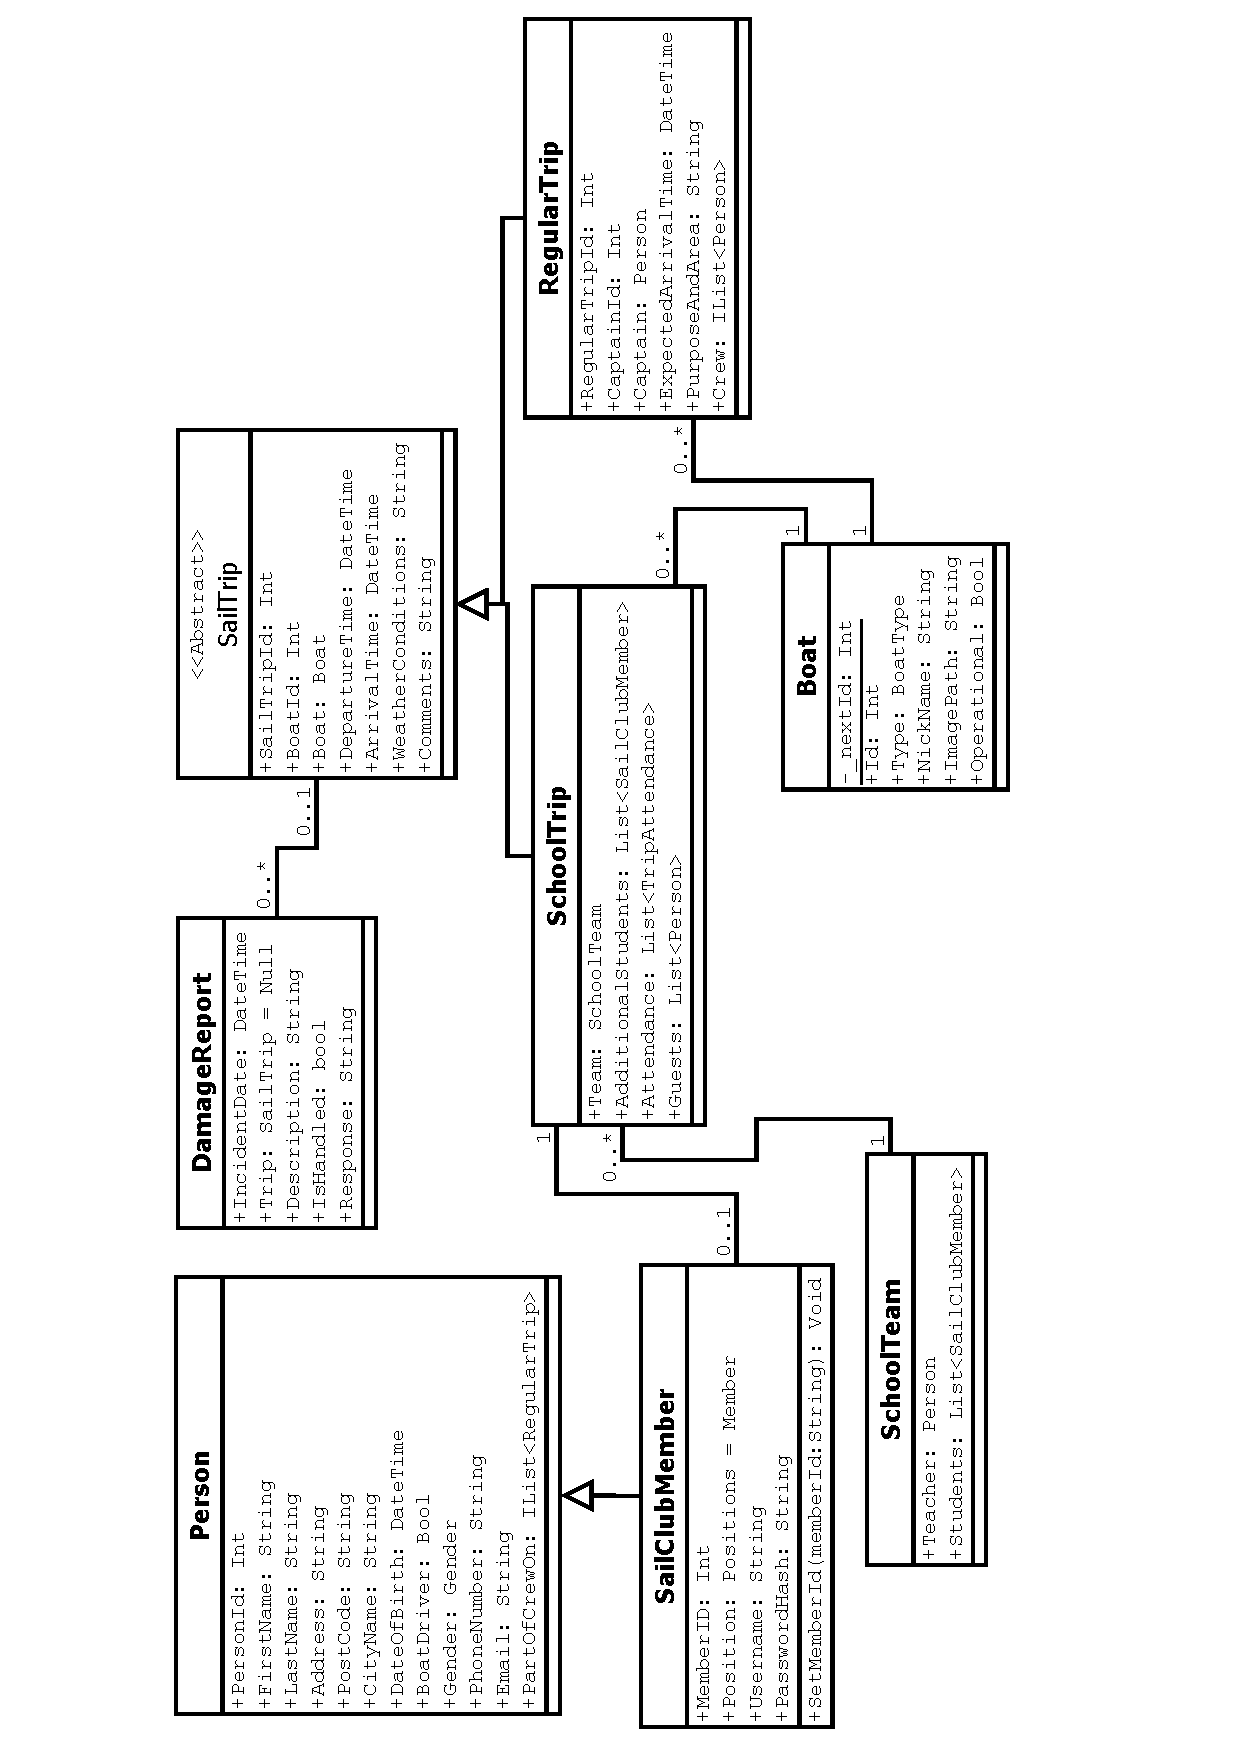
\includegraphics[width=0.70\textwidth]{images/flowcharts/UML.pdf}
  \caption{UML-diagram over klasserne i programmet}
  \label{img:UML}
\end{figure}

\subsection*{Klasse: Person}
\textbf{Formål:}
Formålet med personklassen er at kunne repræsentere personer som vedrører programmet.
Data om disse personer angives som felter i personklassen.

\textbf{Metoder:}
Personklassen har overridet \textbf{ToString()}, som returnerer \textbf{FullName}.

\textbf{Anvendelse:}
Personklassen bruges til at repræsentere alle personer i systemet. 
Gæster repræsenteres direkte som instanser af personklassen. 
Sejlklubbens medlemmer repræsenteres som subklasser af personklassen. 

\subsection*{Klasse: SailClubMember}

\textbf{Formål:}
SailClubMember bruges til at repræsentere medlemmerne i sejlklubben, med undtagelse af de studerende som har en subklasse.

\textbf{Position} feltet angiver hvilken rang, og dermed rettigheder, som et sejlklubmedlem har. 
Dette repræsenteres ud fra en enumeration.

\textbf{Anvendelse:}
SailClubMember bruges til at danne instanser af alle sejlklubbens medlemmer, bortset fra de studerende som er instanser af StudentMember der nedarver fra SailClubMember.

\subsection*{Klasse: StudentMember}
\textbf{Formål:}
Klassen StudentMember indeholder informationer om, hvilke læringsmål eleven har udført i forbindelse med sejlerskolen. 

\textbf{Anvendelse:}
Klassen StudentMember nedarver fra SailClubMember og bruges til at repræsentere eleverne i sejlklubben.

\subsection*{Klasse: Team}

\textbf{Formål:}
Klassen Team har til formål at repræsentere et vilkårligt sejlerskolehold.
Samtidigt inderholder den både en liste over elever og lektioner.

\textbf{Anvendelse:}
Team anvendes til at samle en gruppe elever i sejlerskolen.
Denne samling gør det muligt at håndtere eleverne på holdet på samme tid.

\subsection*{Klasserne: SailTrip og RegularSailTrip}
\textbf{Formål:}
I en tidlig designstruktur var det tænkt at programmet skulle indeholde flere forskellige typer af sejlture, og derfor blev SailTrip-klassen skabt som værende superklasse for sejltursklasser. 
Senere blev ideen om at have flere typer sejlture ændret, og i stedet blev der valgt, at der kun skulle være én sejlturstype. 
SailTrip-klassen er dog bibeholdt i tilfælde af videre udbygning af programmet.
Dog findes der enkelte felter i klasserne, som overlapper hinanden lidt, men felter er også bibeholdt i tilfælde af udbygning til flere typer sejlture.

\textbf{Anvendelse:}
SailTrip-klassen anvendes kun som superklasse for RegularTrip-klassen. 
Hver reservation er en instans af klassen RegularTrip, dette gælder også reservationer for sejlerskolens lektioner.

\subsection*{Klasse: Event}

\textbf{Formål:} 
Denne klasse repræsenterer en begivenhed i sejlklubben.

\textbf{Anvendelse:}
En instans af eventklassen, repræsenterer en begivenhed, der ikke nødvendigvis er sejlrelateret.

\subsection*{Klasse: Logbook}

\textbf{Formål:}
Efter hver sejltur skal der udfyldes en logbog med informationer om sejlturen. 
Denne klasse repræsenterer denne logbog.

\textbf{Anvendelse:}
En instans af klassen Logbook findes på hver sejltur. 
Den udfyldes af personen, som har foretaget reservationen, efter sejladsens fuldførelse. 

\subsection*{Klasse: Lecture}

\textbf{Formål:}
Klassen Lecture indeholder information vedrørende en undervisning. 

\textbf{Anvendelse:}
Denne klasse bruges, når der reserveres en båd til sejlerskolen og samtidigt til at registrere, hvilke læringsmål som blev udført på turen. 


\chapter{Database}

I forbindelse med programmets data var det nødvendigt at overveje, om programmet skulle have foruddefineret
data, som ville blive nulstillet ved hvert programopstart, eller om dataene skulle gemmes mellem kørsler.

Efter nogen overvejelse blev det bestemt, at der skulle benyttes et såkaldt persistenslag. Efter at have
overvejet SQLite og \ac{EF} faldt valget på \ac{EF}, der er populært blandt C\#--udviklere, da det tillader en
hurtig start på kodeprocessen.

\ac{EF} er et såkaldt \ac{ORM} framework, der sammenkæder tabeller i en database med objekter i et program.
Det kan benyttes på flere måder, der kort fortalt afhænger af, om man starter med en defineret database, eller
en samling af klasser. Sidstnævnte mulighed kaldes for ``Code First'' og blev den valgte metode, da det tillod
en -- for gruppen -- logisk arbejdsproces, hvori klassestrukturen blev opbygget, og databasen blev automatisk
tilpasset denne.

Der blev truffet afgørelse i gruppen om at benytte et såkaldt \ac{DAL} til at give programmet yderligere
robusthed. Et \ac{DAL} er en samling af interfaces, samt implementationer af disse, som lægger sig mellem
programmet og det valgte persistenslag. Hermed opnås mulighed for at udskifte persistenslag, eller sågar
benytte flere forskellige i det samme program. Ligeledes bliver det muligt at have et lag specifikt til at
teste med. I yderste konsekvens, hvis det skulle vise sig, af \ac{EF} fejlede, og der ikke kunne rettes op på
det i tide, så ville det være muligt at skrive en såkaldt ``mock implementation'', hvilket ville give den
først overvejede mulighed for at have data, som ikke gemmes i noget lager.

Det er også værd at bemærke, at mange udviklere vælger at benytte \ac{EF} Code First under udviklingen, med en
passende \ac{DAL}--implementation, for derefter, når programmet skal distribueres, at kode en implementation
der benytter en database eller lignende, som de har fuld kontrol over. \ac{EF} har et højt abstraktionsniveau,
hvilket simplificerer arbejdsprocessen, men fratager udvikleren en del kontrol.




\section{Det ``gamle'' --- Bare i tilfælde af, at noget af det skal bruges.}

For at kunne holde på data, imellem kørsler af programmet, skal der været en form for persistens. 
Dette opnåes ved at lagere data. 

Til lagering af data findes der flere måder, den primære overvejse er mellem en database og tekstfiler.
Flade filer, eller såkaldte ``flat files'' på engelsk, er tekstfiler, som bruges til datalagring. 
Flade filer er en meget simpel løsning, som vil være nemt at få i gang, men den skalerer ikke særligt godt. 
%Fordelen ved flade filer er, at de er meget simple at håndtere, hvor databaser på den anden side er mere avanceret at håndtere og programmere. 
%På den anden side var der databaser. Der var under dette valg ikke taget stilling til hvilken type database, som skulle bruges, men bare om der generelt skulle bruges database. 
En database er et stykke software som opbevarer data, på en hensigtsmæssig måde. 
Der findes en lang række af database management systemer (DBMS) hver med fordele og ulemper, mange af dem understøtter Structured Query Language (SQL) standarden.

Med databaser kan der dog være flere muligheder for datahåndtering, og der er også løsninger til C\#, som skulle være til at overkomme at implementere.\citep{flatfiles} 
Af den grund blev der valgt at bruge almindelig database fremfor flade filer. 

Gruppen kiggede nærmere på SQLite og Entity Framework (Code-First). 
SQLite er en serverløs, selvstændig, konfigurationsløs database. 
Dette gør den meget simpel i anvendelse, samt ville resourceforbruget være meget lavt. 
Entity Framework er en object-relational mapping (ORM) framework til .NET platformen. 
Altså får hvert objekt, der ønskes lagret, en plads i databasen. 
Med ``Entity Code First'' arbejdsmodellen, så laves klasser først, hvorefter Entity Framework håndterer integrationen med dens database.

Gruppen adspurte vores underviser i Objet Orienteret Programmering, og han anbefalede Entity Framework (Code-First), til vores problemstilling. 
Valget faldte derfor på Entity Framework, med Code-First mønsteret. 

%Valget af database kom til at stå mellem at bruge SQLite og Entity Framework. SQLite er et databasesystem, som har implementeret det meste af SQL standarderne.
%SQLite blev taget i betragtning, da det skulle være meget simpelt at implementere og bruge og, at det ligeledes er et populært valg til lokal database. 
%Fordelen ved SQLite er dens simpelhed og integration med C\#. 
%På den anden side er der det såkaldte Entity Framework, som er en Object Relational Mapper (ORM) for ADO.NET, hvilket vil sige, at den skaber objekter og entities alt efter databasetabellerne og skaber mekanismer for bl.a. CRUD (Create, Read, Update, Delete) opperationer. \citep{entity} 
%Den måde som Entity Framework regnes med at blive implementeret, er såkaldt ``Entity Code First'', hvilket, som navnet antyder, er at kodningen starter før opsætningen og programmeringen af selve databasen. Der er også mulighed for at lava databasen først, og så kode bagefter.
%Fordelen ved Entity Framework er, som nævnt før, muligheden for at kode først, og derefter lave databasen ud fra det eksisterende kode. 
%Valget faldt på Entity Framwork, da det skulle være simpelt at implementere. Vi var også blevet anbefalet at bruge Entity Framework af vores C\#-lærer.\fxnote{Skal der henvises til vores lærers anbefaling eller bare droppe det?}

%Sammen med Entity Framework, så gøres der brug af et såkaldt Data Abstraction Layer (DAL), hvilket virker som en adskillelse mellem selve koden og databasen, så koden stadig vil virke uden databasen. 
%Ved brug af et DAL, så er det også muligt at teste databasen, bl.a. læse og skrivemuligheder. 

\chapter{Programmets brugergrænseflade}


I dette kapitel vil programmet grafiske brugergrænseflade blive beskrevet.


\section{Navigering i programmet}

\begin{figure}[H]
\hspace*{-2cm}
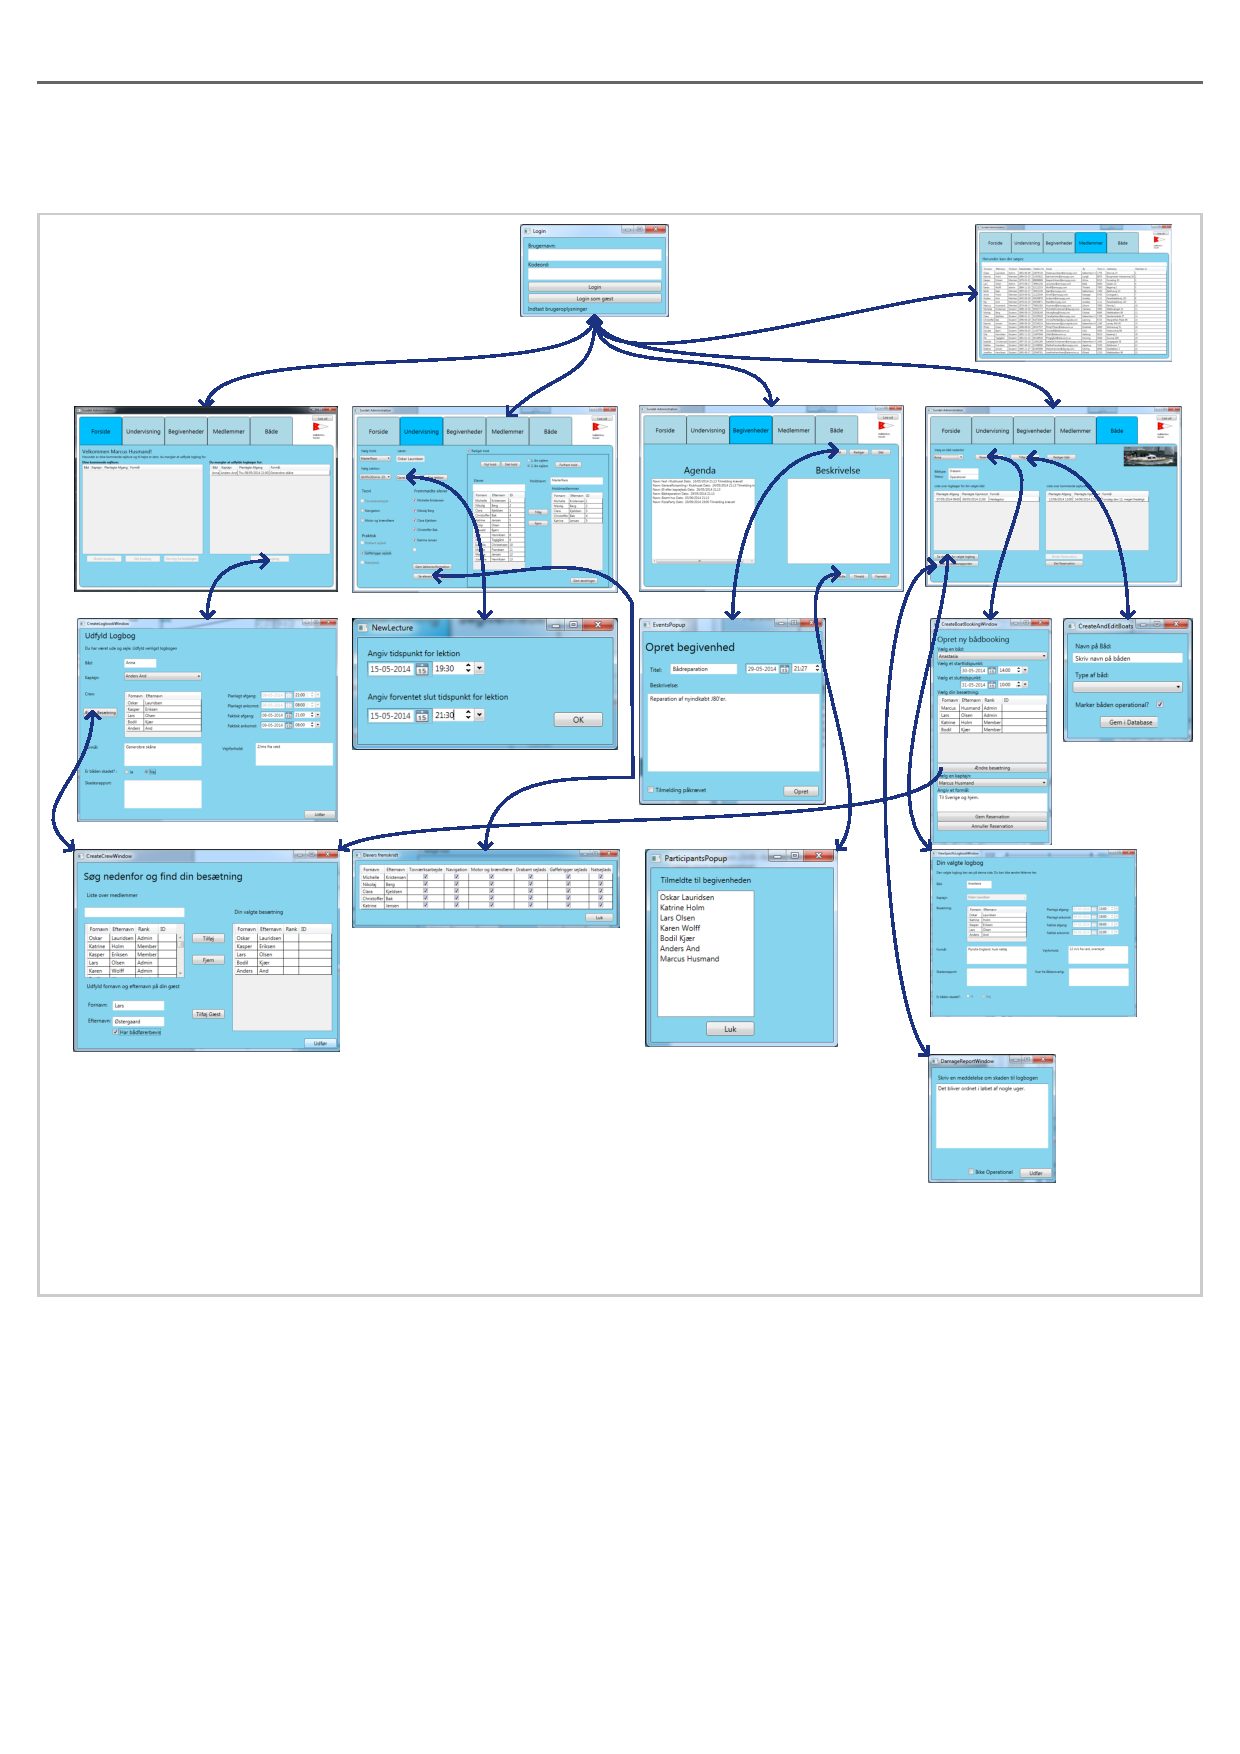
\includegraphics{UI/UI2.pdf}
\vspace{-310pt}
\caption{Navigations skema for programmet}
\label{img:programNavigation}
\vspace{-20pt}
\end{figure}

På \myref{img:programNavigation} ses der hvordan navigeringen i programmet foregår.
Øverst ses login-vinduet, herfra logger brugeren ind med sine login informationer, eller en gæst kan logge ind ved at trykke på \textit{login som gæst}-knappen.
Brugeren ser nu hovedvinduet, hvilket er vinduet i midten med fem tabs i toppen.
Antallet af tabs varierer alt efter hvilken position brugeren har i systemet, hvilket kan ses på \myref{tab:permissions}. 
Fra forside tabben kan der navigeres til de andre tabs, som brugeren har tilgængelig.
Pilene illustrerer de dialogbokse som brugeren kan åbne fra de forskellige tabs.
Dialogboksene åbnes ved at trykke på knapper inde i tabsne, f.eks. under  \textbf{Bådreservation} kan opret booking dialogen åbnes ved at trykke på knappen \textit{Reserver Båden}. 
På samme måde åbnes de resterende dialoger ved tryk på knapper.
Flere steder i programmet anvendes de samme dialogvinduer, f.eks. fra forsiden findes en mulighed for at ændre på en reservation, hvilket åbner en mindre modificeret udgave af booking dialogen, hvorfra besætningsvælgerdialogen også kan åbnes.
Desuden findes logbogsdialogen også på forsiden.
Forskellen på logbogsdialogen på forsiden og den under bådreservation, er at dialogen under forsiden er lavet for at logbogen kan udfyldes, mens den under bådreservation er read-only.
\fxnote{Aner ikke om knapperne har de rigtige navne}



% LaTeX tabel som viser alle brugerniveauer og deres muligheder efter login.
% http://bit.ly/1kToHZ3 to edit raw table
\begin{table}
    \colorlet{shadecolor}{gray!40}
    \rowcolors{1}{white}{shadecolor}
    \begin{tabular}{l|llll}
    \hline
    ~                        & Gæst & Medlem & Elev & Administrator \\ \hline
    Personlig forside        & ~    & \ding{51}      & \ding{51}    & \ding{51}             \\
    Se begivenheder          & \ding{51}    & \ding{51}      & \ding{51}    & \ding{51}             \\
    Tilmeld begivenheder     & ~    & \ding{51}      & \ding{51}    & \ding{51}             \\
    Opret begivenheder       & ~    & ~      & ~    & \ding{51}             \\
    Se sejlture              & \ding{51}    & \ding{51}      & \ding{51}    & \ding{51}             \\
    Opret sejltur            & ~    & \ding{51}      & \ding{51}    & \ding{51}             \\
    Se logbøger              & \ding{51}    & \ding{51}      & \ding{51}    & \ding{51}             \\
    Opret logbog             & ~    & \ding{51}      & \ding{51}    & \ding{51}             \\
    Svar på logbog           & ~    & ~      & ~    & \ding{51}             \\
    Se undervisningstimer    & ~    & ~      & \ding{51}    & \ding{51}             \\
    Opret undervisningstimer & ~    & ~      & ~    & \ding{51}             \\
    \end{tabular}
    \caption{Tabel over alle brugerniveauer og deres tilladte funktioner.}\label{tab:permissions}
\end{table}

\section{Hovedvinduet}
Hovedvinduet tilgås via loginvinduet, som starter ved programstart eller ved at trykke på logudknappen inde fra hovedvinduet selv. 
Der findes fire udgaver af hovedvinduet, forskellen mellem dem er, hvilke tabs der er aktive.
Hver tab indeholder forskellige funktioner, samlet set findes følgende tabs:
\begin{itemize}% Denne skulle måske relatere til tabel tab:permission
    \item Forside
    \item Undervisning
    \item Begivenheder
    \item Medlemmer
    \item Både
\end{itemize}

Via hver af disse tabs, vil der være adgang til programmets forskellige funktionaliteter.
Der er også en logud knap, som bruges til at vende tilbage til loginvinduet, således en anden bruger kan anvende systemet.
Programmet er lavet til at køre i opløsningen 1024x720 pixels.
Denne opløsning er valgt for at understøtte alt fra bærbare, med opløsninger som 1366x768 pixels i et vindue, og op til FullHD (1920x1080 pixels) op op efter. 
Stort set alle computerskærme har en opløsning større end 1024x720 pixels\citep{resolutions}. 
Programmet har et lyst farveskema; med farverne hvid og en lys blå som hovedfarver (\#87D4EE).

\section{UserControls}
Der anvendes Usercontrols til at kode både brugergrænsefladen og den tilhørende Code-Behind.

\subsection{DateTimePicker}\label{subsec:DateTimePicker}

\begin{wrapfigure}{r}{0.5\textwidth}
    \label{img:DateTimePicker}
    \vspace{-20pt}
    \begin{center}
        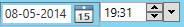
\includegraphics[width=0.48\textwidth]{Screenshots/DateTimePicker.png}
    \end{center}
    \vspace{-15pt}
    \caption{DateTimePicker}
    \vspace{-30pt}
\end{wrapfigure}

\textbf{Formål}: 
Denne Usercontrol er lavet, da der ikke fandtes en tilfredsstillende løsning, som gjorde det muligt at vælge både dato og tidspunkt i samme control. 
Det er ofte nødvendigt at vælge både dato og tidspunkt samtidigt. 

\textbf{BrugerGrænseflade}: 
Den består af en DatePicker, og en TimePicker som findes i extended WPF toolkit.

\textbf{Code-Behind}: 
Der er blevet lavet en specialfremstillet getter og setter for Usercontrolen. 


\subsection{Forside}

\textbf{Formål}: 
Formålet med forsiden er at vise aktuel infomation på en overskuelig måde for brugeren.
Det er den første side i hovedvinduet, som man ser, med mindre man er gæst.
Fra forsiden kan man ændre og slette sine bookings, samt starte oprettelsen af en logbog.

\textbf{Brugergrænseflade}: 
Brugergrænsefladen på forsiden består primært af to DataGrids: Det venstre viser dine kommende sejlture, og det højre viser de sejlture personen mangler at udfylde logbøger for. 
Under dem er der knapper, som bliver aktive efter en markering er udført ved, at trykke på en af rækkerne i det tilhørende datagrid.

\textbf{Code-Behind}: 
For kun at vise de sejlture hvor personen, som er logget ind deltager i, anvendes der standard query operatorer. 
I listing \ref{fntpg-cb} er der et udsnit af koden, nærmere bestemt den del som vælger de korrekte sejlture.

Begge udtryk returnerer en IEnumerable, som derefter assignes som DataGridenes ItemSource.

\begin{lstlisting}[frame=single, caption=Forsidens Code-Behind, label=fntpg-cb]
//Sets the trips for the person currently logged in while only getting the ones in the furture to the DataGrid ItemsSource
UpcommingTripsDataGrid.ItemsSource =
    sailTripList.Where(t => t.Crew.Select(p => p.PersonId).Contains(usrId))
        .Where(t => t.DepartureTime > DateTime.Now);
//Sets trips created by the current user which happend in the past while also missing a logbook, to the other DataGrid ItemsSource 
LogbookDataGrid.ItemsSource =
    sailTripList.Where(t => t.Captain.PersonId == usrId && t.ArrivalTime < DateTime.Now && t.Logbook == null);
\end{lstlisting}

\subsection{Boat UserControl}

\textbf{Formål:}
I fanebladet Både kan man få et overblik over hvilke både som, der er til rådighed i sejlklubben inklusiv bådtype og status på båden. 
Man kan også booke en båd, se liste over logbøger for en valgt båd og ligeledes se en liste over kommende reservationer. 

\textbf{Brugergrænseflade:}
Efter valg af båd opdateres de resterende elementer i UserControlen. 
Her kan der ses et DataGrid med udfyldte logbøger samt et andet DataGrid med kommende reservationer på båden.
Det er muligt at vise og ændre felterne i begge DataGrids.
Som administrator kan man også svare på logbogens skadesrapport.
Foruden disse funktionaliteter kan man også herinde reserver den valgte båd samt har administratorer mulighed for at tilføje og redigere både.

\textbf{Code-Behind:}
Den bagvedliggende kode henter data fra databasen og opdaterer de grafiske elementer med dataet. 


\subsection{StudyTeacher UserControl}

\textbf{Formål:}
Denne UserControl bruges til give lærerer på sejlerskolen mulighed for at administrere skolehold og undervisningslektioner.

\textbf{Brugergrænseflade:}
Når der er valgt et hold, er der forskellige controls som opdateres.
Man kan se holdets lærer, elever og hvorvidt holdet er et 1. eller 2. års hold. 
Det er også muligt at se holdets lektioner, samt oprette og slette disse.
Når der trykkes på knappen for opretning af en ny lektion, åbnes et nyt vindue, hvor man indtaster start og sluttidspunkt.
Efter der er valgt en lektion kan der afkrydset hvad der er lært på lektionen, samt hvilke elever der har lært disse.
Der er også en knap som åbner et vindue, hvor man kan se hvilke læringsområder de enkelte elever har lært.
Når der laves et nyt hold, åbnes et vindue hvor man blot indtaster det ønskede navn for holdet.
Der kan slettes og forfremmes hold, hvilket betyder de får et bådførerbevis.

\textbf{Code-Behind:}
Når der oprettes en lektion, bliver der reserveret en båd på det pågældende tidspunkt.
Når der forsøges at forfremme et hold, tjekker Code-Behinden om eleverne har lært alt det de skal og ændrer herefter eleverne fra StudentMember til SailClubMember og sætter deres BoatDriver property til true.

Der findes også en undervisnings UserControl for elever. 
Denne kan ikke interageres med men viser blot hvilke læringsområde eleverne har lært, informationer om det hold de er på, samt hvornår næste lektion er.

\subsection{Event UserControl}
\textbf{Formål:}
UserControlen Event bruges til at se informationer om kommende begivenheder i sejlklubben. 
Hvis man er administrator kan også oprettes nye begivenheder, redigering og sletning af eksisterende begivenheder og tilmelding hvis det kræves.

\textbf{Brugergrænseflade:}
Brugergrænsefladen består mest af to ListBoxe.
I den første bliver begivenheder vist med navn, dato og om der kræves tilmelding.
I den næste ListBox vises beskrivelsen af begivenheden når der klikkes på en begivenhed i den tidligere ListBox. 

\textbf{Code-Behind:}
Den bagvedliggende kode henter allerede oprettede begivenheder fra databasen. 
Ved oprettelse, redigering og sletning skrives ændringerne til databasen. 
Ved tilmelding tilføjes personen, som er logget ind, til listen over tilmeldte personer, som hver Event har instansieret. 

\section{Vinduer}
Aller vinduer beskrevet i dette afsnit kan ses på \myref{img:programNavigation}. 

\subsection{Login brugergrænseflade}
 
\textbf{Formål}:
Login brugergrænsefladen har til formål at verificere en brugers identitet. 
Det er det første vindue brugeren ser når programmet åbnes, og det åbner hovedvinduet efter fuldført login.
 
\textbf{BrugerGrænseflade}: 
Brugergrænsefladen til loginvinduet er meget simpel og ligetil. 
Der er en TextBox til brugernavnet og en PasswordBox til kodeordet.
En PasswordBox er en TextBox, hvor hver af de indtastede karakterer vises som en sort prik, i stedet for de skrevne tegn, for at beskytte brugeren.
``Login som gæst''-knappen kræver ingen brugeroplysninger og åbner en let udgave af hovedvinduet, uden særlige tilladelser.
Til sidst er en TextBlock, som fortæller brugeren, hvad der er skrevet forkert, hvis der er skrevet noget forkert.

\textbf{Code-Behind}: 
TextBoxen, hvor brugernavnet indtastes, er case insensitive.
PasswordTextBoxen er case sensitive. 

\subsection{CreateBoatBookingWindow}
\textbf{Formål}: 
Dette vindue opretter, eller ændrer, en instans af RegularTrip.

\textbf{Brugergrænseflade}: 
Først vælges en båd, her anvendes en ComboBox.
Herefter anvendes \textbf{DateTimePicker}-UserControllen til at vælge et start- og sluttidspunkt.
Der vises den nuværende besætning, samt muligheden for at ændre den ved at trykke på en knappen ``Ændre Besætning'', som åbner CreateCrewWindow.
Når en besætning er valgt, kan der vælges en kaptajn ud fra besætningslisten.
Til sidst er der en TextBox, hvori brugeren kan angive formålet med turen.

\textbf{Code-Behind}: 
I Code-Behinden er der to constructors. 
Den ene bruges til at oprette en ny reservation, den anden bruges når der skal ændres på en eksisterende reservation. 
Efter tryk på ``Gem Reservation'', verificeres brugerens input fra alle de grafiske elementer i vinduet.

\subsection{CreateCrewWindow}

\textbf{Formål}: Dette vindue åbnes to steder i programmet: \textbf{CreateLogbookWindow} og i \textbf{CreateBoatBookingWindow}. 
Det bruges, når der skal laves en besætning til en RegularTrip.  

\textbf{Brugergrænseflade}: 
Der er to DataGrids, som hver indeholder en liste. 
Listen til venstre består af SailClubMembers, som bliver hentet ind fra databasen. 
Listen til højre indeholder det Crew, som man er i gang med at udforme til enten RegularTrip eller Logbook. 
Der er også tilføjet TextBoxe, så man kan skrive navnet på en gæst, man tog med på sejlturen. 
Der er knapper, som tilføjer de forskellige personer til Crewlisten. 
Øverst findes også et tekstfelt til at søge i listen over medlemmer. 
Når man har lavet sin liste, kan man trykke udfør, for at komme tilbage til vinduet, der kaldte CreateCrewWindow.

\textbf{Code-Behind}: 
Der er blevet brugt et \textbf{regular expression} til at tjekke, om den string brugeren angiver i de to TextBoxe for gæstens navne, er lovlige. 
Det er blevet valgt, at man må bruge hele det danske alfabet samt mellemrum, så navne såsom: Lars Peter Østergaard, er mulige.
Derefter tilføjes personen til listen, der vises i DataGridet til højre, og til sidst kaldes RefreshDataGrid, som man kan se på \myref{RefreshDatagrid}.

Her modtages der et DataGrid, som skal have dets Itemssource opdateret, og en ICollection, som er det data, der skal sættes ind i DataGridet. 
Det gøres ved at assigne dets ItemsSource til null, og derefter assigne det tilbage til den ICollection, der blev sendt med. 
Der kan laves en tilsvarende metode, som opdaterer andre WPF-controls.

\begin{lstlisting}[frame=single, caption=Refresh Datagrid, label=RefreshDatagrid]
private void RefreshDatagrid(DataGrid Grid, ICollection<Person> list)
{
    Grid.ItemsSource = null;
    Grid.ItemsSource = list;
}
\end{lstlisting}

\subsection{CreateLogbookWindow}

\textbf{Formål}: 
Dette vindue bruges til at udfylde logbogen for en sejltur.

\textbf{Brugergrænseflade}:  
Når vinduet åbnes indlæses der data fra den instans af RegularTrip som logbogen udfyldes for.
Som tidligere vinduer, bliver dataet afbilledet i de respektive grafiske elementer. 
De tomme felter skal selv udfyldes af brugeren. 

\textbf{Code-Behind}: 
Code-Behinden verificerer dataet inden det gemmes i databasen.
Herudover sættes referencen til logbogen i det pågældende RegularTrip.


\chapter{Test af program}\label{test_af_program}
I dette kapitel, beskrives de to typer af tests der er udført i forbindelse med projektet.

\section{Unit test}
Til test af selve koden er der benyttet Unit tests.
Unit tests tester metoder, properties, klasser og assemblies. 
Når man har lavet en metode, så forventer man, som regel, et bestemt resultat.
Unit test af metoden fungerer ved, at man giver metoden, som skal testes, et input, og ser man får det forventede resultat.

Til Unit tests bruges frameworket NUnit, som er lavet til .NET platformen. 
Det er ikke alt kode, som bliver testet, men udvalgte kodestykker.
Disse udvalgte kodestykker er valgt på baggrund af deres relevans for den overordnede struktur i programmet. 
Blandt andet bliver klasserne testet.

Et eksempel på en unit test kan ses på \myref{unit_test}.
Først bliver MemberId sat til værdien 3. 
Derefter bliver der vha. \texttt{Assert.AreEqual} tjekket, om SailClubMemberId bliver sat til værdien 3.
Hvis den bliver sat til værdien 3, så består testen.

\begin{lstlisting}[frame=single, caption=Eksempel på Unit test, label=unit_test]
        [Test]
        public void SetMemberId_InputSimpleNumberString_ShouldSetMemberIdToNumericValue()
        {
            this.SetMemberId("3");
            Assert.AreEqual(3, this.SailClubMemberId);
        }
\end{lstlisting}

\section{Brugertest}
I dette afsnit forklares fremgangsmåden for brugertests i forbindelse med programmets brugervenlighed.
Derudover ses der nærmere på hvordan resultaterne bruges, hvorfra der kan dannes et overblik over programmets funktionalitet. 

For at teste programmet anvendes der, foruden unit tests i dette projekt, en række brugertests, som tager udgangspunkt i projektets UserStories\myref{User_stories}.
Denne type test ligger fokus på uafhængige brugers mening om programmets brugervenlighed.

For at teste programmet anvendes der, foruden unit tests i dette projekt, en række brugertests, som tager udgangspunkt i projektets UserStories\fxnote{myref til userstories}. 
Denne type test ligger fokus på uafhængige brugers, dvs. brugere som ingen association til hverken gruppen eller projektet, mening om programmets brugervenlighed.
Testens form er inspireret af black-box testing, som normalt ellers udføres af udviklerne selv.

Da programmet er lavet med henblik på brug i en sejlklub, består målgruppen af mange forskellige befolkningssegmenter. 
Idet det er et computerprogram, er det eneste krav til målgruppen, at det er villige til at bruge en computer.

Ud fra programmets funktionaliteter dannes der nogle mål som brugerene skal opnå igennem testen. 
Der defineres en række testscenarier med udgangspunkt i de mål der blev sat for testen.
Disse mål er:
\begin{itemize}
  \item Følge sin undervisningsstatus.
  \item Se reservationer af både.
  \item Oprette reservation af både.
  \item Tilmelde sig begivenheder.
  \item Følge status på begivenheder og undervisning.
  \item Oprette logbog for fuldendt sejlads.
\end{itemize}

Ud fra disse mål er der skrevet en række korte opgaver, som berører bestemte funktionaliteter i programmet. 
Opgaverne kan findes i \myref{BrugerTestCases}.

Dette bilag vil blive vist til testpersoner af programmet, og de vil blive observeret under testen. 
Efter udførslen af testen spørges der ind til brugerens oplevelse af programmet med henblik på funktionalitet, brugergrænseflades design, og deres helhedsindtryk.

En opgave kunne eksempelvis være:
\begin{itemize}
	\item Log ind på systemet med følgende brugeroplysninger: oskar og lauridsen
	\item Foretag en booking af båden: Anna til næste lørdag, med følgende andre oplysninger: 
	\begin{itemize}
		\item Starttidspunkt: 20-07-2014 13:37
		\item Sluttidspunkt: 20-07-2014 20:42
		\item Besætning: Jens Hansen, Anders And\ldots
		\item Kaptajn: Anders And
		\item Formål: Eftermiddagssejlads
	\end{itemize}
	\item Log ud af systemet igen
\end{itemize}

Samtidigt udfyldes et skema med tidsforbrug af hver enkelt opgave, samt kommentarer omkring brugerens færden i programmet.

I de følgende afsnit beskrives der hvordan testens data vil blive behandlet.

\subsection{Funktionalitet}
I testområdet funktionalitet undersøges der hvorvidt opgaverne stillet er mulige at løse for testpersonerne.
Dermed testes der om brugergrænsefladen hindrer programmets funktionalitet. 

\subsection{Effektivitet}
Effektivitet anses som værende forholdet mellem en ekspert og en nybegynders tid, for at udføre en given opgave.\citep{UIEffeciency}
Derfor tages der tid på udførelsen af, hver enkelt opgave som testpersonen udfører.
Eksperten vil være et medlem af projektgruppen, som ikke var observatør i nogen af de andre testpersoners test. 

\subsection{Tilfredshed}
Til sidst laves der en tilfredshedsundersøgelse for at få brugerens meninger omkring programmets design. 
Dette gøres igennem et spørgeskema. 
Undersøgelsen skal give et indtryk af, hvor godt brugeren synes programmet var i forhold til layout, placering og synlighed af de krævede elementer i programmet. 
Denne undersøgelse giver et indtryk af, hvor godt programmet er designet, og sværhedsgraden af forskellige funktioner. 
Spørgeskemaet kan ses i \myref{bilag:SporgeSkema}. \citep{UISatisfaction}


\section{Analyse af testresultater}

Grundet tidspres bl.a. fra fejl med databasen, var der kun tid til at teste på fire personer, samt eksperten.
Personerne der udførte testene, bestod af elever på Aalborg Universitet, som ikke havde set eller på anden vis hørt om projektet før.
Resultaterne kan ikke konkluderes til at give et endegyldigt svar på om programmet kan bruges i sejlklubben Sundet, da de ingen kendskab har til sejlklubben, og deres behov.
For at få et mere brugbart resultat fra testen, skulle testpersonerne være en repræsentativ gruppe af medlemmer fra sejlklubben, eller på anden vis være indblandet med en sejlklub. 
På denne måde, ville testpersonen have en bedre forståelse for, kravene til programmets funktionalitet.
Dog menes det at testens resultater alligevel kan sige noget om brugen af programmet, både om navigering og de testede funktioner.
\subsection{TestData}
På \myref{tab:TestTimeTable} kan der ses en tabel over tid brugt ved hver opgave for hver enkelt testperson, sammenlignet med ekspertens tid.

% Table generated by Excel2LaTeX from sheet 'Sheet1'
\begin{table}[htbp]
    \colorlet{shadecolor}{gray!40}
    \rowcolors{1}{white}{shadecolor}
  \centering
  \caption{Tid brugt pr opgave under test. T[1-4] er udefrakommende testpersoner.}
    \begin{tabular}{r|rrrr|r|r|r}
    \textbf{Opgave} & T1     & T2     & T3     & T4     & \textbf{AVG} & \textbf{Ekspert} & \textbf{Sammenligning} \\ \hline
    1     & 00:15 & 00:32 & 00:24 & 00:31 & 00:25 & 00:15 & 59\% \\
    2     & 04:42 & 04:00 & 02:04 & 02:27 & 03:18 & 01:35 & 48\% \\
    3     & 01:08 & 02:13 & 01:02 & 01:10 & 01:23 & 00:30 & 36\% \\
    4     & 00:49 & 00:32 & 00:32 & 00:55 & 00:42 & 00:29 & 69\% \\
    5     & 00:29 & 00:24 & 00:27 & 00:30 & 00:27 & 00:13 & 47\% \\
    6     & 01:16 & 00:57 & 00:57 & 01:02 & 01:03 & 00:50 & 79\% \\
    7     & 02:00 & 00:35 & 00:30 & 00:40 & 00:56 & 00:14 & 25\% \\
    8     & 02:02 & 04:20 & 04:57 & 02:10 & 03:22 & 00:56 & 28\% \\
    9     & 00:32 & 00:26 & 00:19 & 00:42 & 00:29 & 00:10 & 34\% \\ \hline
    \textbf{SUM} & 11:56 & 13:59 & 11:12 & 10:07 & 11:48 & 05:12 & 44\% \\
    %\bottomrule
    \end{tabular}%
  \label{tab:TestTimeTable}%
\end{table}%

Det lykkedes for testpersonerne at udføre alle opgaverne.

\subsection{Diskussion af test data}

Nogle opgaver var tydeligt sværere end andre for personer som ikke havde kendskab til programmets brugergrænseflade. 
Særligt var opgave 2, 7, og 8 udfordrende.


Opgave 2 lød på at reservere en bestemt båd, med udleverede data.
Den tiltænkte løsning af opgaven er:
\begin{enumerate}
    \item Vælg tabben ``Både''
    \item Vælg båden ``Anastasia''
    \item Tryk på knappen ``Reserver båden'' (Dette åbner CreateBoatBookingWindow)
    \item Udfyld felterne med det udleverede data.
    \item Tryk på knappen ``Gem reservation''
\end{enumerate}

T1 og T2 havde svært ved det 3. skridt i opgaven.
Fælles var at de havde brugt over to minutter på netop dette skridt.
Efter udførelse af testen blev de bedt om at uddybe, hvorfor dette var sådan.
De mente begge at der var for meget støj på tabben ``Både'' og dette distraherede dem fra at finde den korrekte knap.
T3 og T4 havde i kontrast ingen problemer med at gennemgå dette skridt, og brugte hver under fem sekunder på at finde den korrekte knap. 
Eksperten brugte væsentligt mindre tid end T1 og T2, men sammenlignet T3 er forskellen betydeligt mindre.

\textbf{Testpersonernes forslag til forbedring af funktionalitet i denne opgave:}
\begin{itemize}
    \item Ryd op i tabben ``Både''. 
    \item Herunder flyt alt logbogsrelateret til sin egen tab.
    \item Øg størrelsen på knappen ``Reserver båden''.
\end{itemize}

I opgave 7 skulle testpersonerne forfremme et hold i sejlerskolen. 
Den tiltænkte løsning af opgaven er:
\begin{enumerate}
    \item Vælg tabben ``Undervisning''
    \item Vælg holdet ``MasterRace''
    \item Tjek CheckBoxen ``Rediger hold''
    \item Tryk på knappen ``Forfrem hold''
    \item Tryk på knappen ``Log ud''
\end{enumerate}

T1 havde særlig svært ved regne ud, at man skal udføre det 3. skridt, før man kunne udføre det 4. skridt.
T1 mente at der var for mange elementer i tabben ``Undervisning'' og at dette forvirrede ham fra at udføre opgaven, da de fjernede opmærksomheden fra CheckBoxen i toppen af tabben.

\textbf{Testpersonernes forslag til forbedring af funktionalitet i denne opgave:}
\begin{itemize}
    \item Flyt rediger hold funktionaliteten til sit eget vindue, ved tryk på en knap.
    \item Der er ingen respons fra programmet efter det 4. skridt, tilføj et popup vindue som giver besked.
\end{itemize}


I opgave 8 blev testpersonerne bedt om at udfylde logbogen for en fuldført tur, som brugeren de anvendt havde reserveret, og derfor skulle udføre logbogen for.

Den tiltænkte løsning af opgaven er:
\begin{enumerate}
    \item Log ind
    \item Marker bådturen i det højre DataGrid på forsiden.
    \item Tryk på knappen ``Opret logbog''
    \item Tryk på knappen ``Ændre besætning''
    \item Fjern ``Kasper Eriksen''
    \item Ændre ``Faktisk afgang''
    \item Tryk på ``Ja'' under ``Er båden skadet?''
    \item Angiv vejrforhold og skadesrapport
    \item Tryk på knappen ``Udfør''
\end{enumerate}

Alle fire testpersoner havde svært ved skridt 2 og 3.
Særligt T2 og T3 brugte lang tid på dette problem.
Testpersonerne besøgte tabben ``Både'' for at udføre dette. 
Eksperten havde ingen problemer med denne opgave og gennemførte opgaven på under et minut.

\textbf{Testpersonernes forslag til forbedring af funktionalitet i denne opgave:}
\begin{itemize}
    \item Giv tydelig besked og instrukser efter log in, om at en logbog mangler at blive udfyldt.
    \item Forøg størrelsen af den forklarende tekst på forsiden til hver af de to DataGrids.
    \item Øg afstanden fra velkomstbeskeden til de 2 DataGrids
    \item Mindske højden af de to DataGrids, da de alligevel er hovedsageligt tomme. 
    \item Dediker en tab til læsning og udførelse af logbøger. 
\end{itemize}

\subsection{Testpersonernes samlede vurdering}

I spørgeskemaet blev testpersonerne bedt om at vurdere flere centrale skærmvinduer.
De blev bedt om at vurdere, deres evne til at overskue hvert af de angivne skærmvinduers funktionaliteter.
Dette skulle angives som en karakter fra et til fem, hvor et er meget uoverskueligt og fem er meget overskueligt.
Dette kan ses i skemaet \myref{tab:vurderingtest}.

% Table generated by Excel2LaTeX from sheet 'Sheet1'
\begin{table}[htbp]
    \colorlet{shadecolor}{gray!40}
    \rowcolors{1}{white}{shadecolor}
    \centering
    \caption{Testpersonernes vurdering af centrale skærmvinduer}
    \begin{tabular}{l|rrrr|r}
        \toprule
        \textbf{Vindue} & T1 & T2 & T3 & T4 & \textbf{GNS} \\
        \midrule
        Forside & 5 & 4 & 4 & 3 & 4 \\
        Undervisning & 1 & 2 & 3 & 2 & 2 \\
        Medlemmer & 4 & 5 & 4 & 2 & 3,75 \\
        Både & 3 & 4 & 3 & 3 & 3,25 \\
        Begivenheder & 4 & 4 & 3 & 2 & 3,25 \\
        Logbogsvinduer & 3 & 2 & 2 & 4 & 2,75 \\
        CreateCrewWindow & 5 & 5 & 4 & 3 & 4,25 \\
        CreateBoatBookingWindow & 5 & 5 & 4 & 4 & 4,5 \\ \hline
        \textbf{Samlet Vurdering} & 3,75 & 3,88 & 3,38 & 2,88 & 3,47 \\
    \end{tabular}%
    \label{tab:vurderingtest}%
\end{table}%

\subsubsection*{Kommentarer fra testpersonerne}
Foruden \myref{tab:vurderingtest} argumenterede testpersonerne også for deres vurdering.

\textbf{Forside}: 
Generelt kunne testpersonerne lide formålet med forsiden, som er at give brugeren et hurtigt overblik efter log in. 
Dog mente flere at layoutet kunne have været udført bedre.
Herunder større afstand fra velkomstteksten til de to DataGrids, større overskrifter ved hver DataGrid, mindre DataGrids da de hovedsageligt var tomme. 

\textbf{Undervisning}: 
Generel utilfredshed omkring denne UserControl.
Specifikt var der klager om at der var CheckBoxes til at tjekke elevers deltagelse af. 
Her mente flere at CreateCrewWindow-vinduet kunne have været anvendt. 
Derudover tilføjede den højre side af vinduet, der havde et layout som lignede CreateCrewWindow-vinduet, forvirring. 
Der var også negative kommentarer omhandlende CheckBoxen ``Rediger hold''. 
Flere fandt denne unødvendig, mens en anden mente af det indhold denne låste op for, burde have sit eget dedikerede popup vindue.

\textbf{Medlemmer}:
Testpersonerne skulle ikke bruge dette vindue i nogen af de stilne opgaver.
Derfor fik de vist dette vindue efter testens gennemførsel, så ledes de kunne kommentere tabbens indhold. 
Der var generelt positive kommentarer, dog mente T4, at den store mænge data virkede overvældende. 
T3 og T4 mente at søgebaren ikke var klart nok markeret, og foreslog at der kunne tilføjes et ``loop''-ikon. 

\textbf{Både}:
Flere testpersoner udtrykte at denne UserControl var uoverskuelig, da der vises for meget information efter valg af en båd.
T1, T3 og T4 forslog at flytte alt logbogsrelateret til sin egen tab.
Derudover kunne størrelsen af skrift forstøres, således den ville være nemmere at læse. 

\textbf{Begivenheder}:
Kommentarer til denne tab var få, T3 forslog at ændre overskriften ``Agenda'' til ``Begivenheder'', over ListBoxen.
Flere mente at brugen af ListBoxen burde have været erstatte med et DataGrid, som er anvendte mange andre steder i programmet. 

\textbf{Logbogsvinduerne}:
Kritikken af disse var primært rettet mod navigeringen til vinduet. 
Der var uenighed imellem testpersonernes vurdering af vinduets design, en mente at elementene i det 2 spaltede layout var uoverskueligt, særligt pga. rækkefølgen af disse. 
Mens en anden udtrykte positive tanker om layoutet.

\textbf{CreateCrewWindow}
Om dette vindue var der næsten kun positive kommentarer.
Vinduet blev omtalt som værende overskueligt, dog kunne DataGridet til venstre godt have været større.
T3 foreslog at dette kunne have samme størrelse med det til venstre. 
Her blev søgefunktionen igen overset, igen blev der foreslået tilføjelsen af et ``loop''-ikon.

\textbf{CreateBoatBookingWindow}
Der var meget få kritikpunkter til dette vindue.
T4 mente at knapperne ``Gem reservation'' og ``Annuller reservation'' var for brede, og burde være placeret således de lignede dem fra windows vinduer såsom egenskaber. 
Altså hvor de er placeret nederst i højre hjørne, på linje med hinanden. 

\subsection{Konklusion af brugertest}
Brugertesten har givet os en større indsigt i programmets layout.
Målene for layoutet var minimalisme og konsistens, men dette er ikke sket, da problemer i arbejdsprocessen, se \myref{sec:faktiske-arbejdsproces}.

På baggrund af brugertesten, etableres det at nogle dele af brugergrænsefladen er bedre konstrueret end andre.
De bedste vurderes til at være vinduerne: \textbf{CreateCrewWindow} og \textbf{CreateBoatBookingWindow}. 
Disse vinduer har begge en høj overskuelighed, dette er et af principperne fra minimalisme, altså at fjerne det unødvendige. 

Ud fra testpersonernes kommentarer kunne de resterende vinduers og UserControls layout forbedres. 
Særligt skulle tabben ``Undervisning'' og tabben ``Både'' forbedres.
Konkrete forslag til disse forbedringer er givet af testpersonerne, disse udtrykker projektgruppen enighed i. 

Men da projektgruppen ikke har en begrænset mænge tid, bliver disse rettelser ikke implementeret. 


\makeatletter\@openrightfalse
\let\cleardoublepage\clearpage
\part{Refleksion}
\chapter{Diskussion}

I diskussionen vil alle elementer fra problemløsningen blive diskuteret. \fxnote{Troels: Her sammenligner vi krav og hvorvidt de er opfyldt. Mere beskrivende metatekst ellers er den useless.}

Et af kravene til produktet var medlemshåndtering, som er implementeret i klasserne Person, SailClubMember og StudentMember. \fxnote{Troels: At vi har klasserne gør os ikke i stand til at sige at systemet håndterer medlemmer, kun hvis der er persistens, som der står i næste linje.}
Derudover lagres objekterne i databasen. 

Medlemmerne udgør desuden grundlaget for login-systemet, da der herigennem kan bestemmes hvilken bruger der logger ind, og hvilke funktioner i programmet de skal have lov til at tilgå.  
Denne løsning ses som værende tilstrækkelig, da det er muligt at registrere hvem som er logget ind og dermed give dem adgang til de respektive funktionaliteter. 

Et vigtigt punkt i programmet var at sørge for at man kunne oprette en reservation af en båd. 
Dette punkt er blevet gennemført, da der i programmet kan oprettes en reservation. 
Desuden er der indført logik, som sikrer at båden skal være ledig og ikke være skadet før reservationen kan gennemføres. \fxnote{Findes dette tjek??? - skadet(Søren) Troels: Ja! }
Yderligere er der til en reservation også knyttet en logbog, som skal udfyldes, efter sejladsen er gennemført. 
Udfyldelsen af logbøger blev beskrevet i interviewet med Jacob Nørbjerg, som værende besværligt i Sejlklubben Sundet, da deres logbøger skal udfyldes på papir. 
Det menes derfor at det udviklede program kan gøre det lettere for klubben at holde styr på logbøger, ved at digitalisere dem, holde referencer til hvilken sejltur de hører til, sørge for at ikke alle kan udfylde logbøgerne og ikke mindst indeholde de krævede informationer. 
Dette anses for at være en god løsning, sammenlignet med at skulle finde den korrekte, fysiske logbog i klubhuset for den pågældende båd og derefter udfylde alle informationerne i hånden. 

Et andet vigtigt krav til programmet var at gøre det muligt at holde styr på undervisningen, både fra elevernes side og undervisernes side. 
I programmet er der blevet konstrueret en del som specifikt tager sig af undervisningen, hvorfra underviserne kan notere hvilke hold og elever der har gennemført specifikke opgaver.
Tilsvarende kan eleverne se deres egne fremskridt og hvornår de har deres undervisningslektioner.
Programmets undervisningsdel fungerer, dog er det specifikke pensum, som sejlklubben Sundet selv står for at udvælge, ikke implementeret. 
Det menes, at skiftet fra det overfladiske pensum, som programmet er skabt med, til det faktiske pensum som Sejlklubben Sundet anvender, ville være relativt simpelt. 
Derfor kan programmet også bruges i andre sejlklubber med undervisning, som anvender et andet pensum.\fxnote{Det kunne dog udvides ved også at holde styr på antallet af gange en elev har udført en given opgave, og ikke kun notere om eleven ahr duført opgaven før.(Søren)}

Begivenheder findes også på listen af produktkrav.
Funktionaliteten for begivenhedshåndtering er blevet implementeret, og det er muligt for brugere selv at oprette, samt tilmelde sig begivenheder.
Desuden kan en bruger, når de logger ind på systemet, se kommende begivenheder og hvilke andre medlemmer der er tilmeldt, hvis begivenheden kræver tilmelding. 
Dette ses som en god løsning, da medlemmer hurtigt kan få et overblik over kommende begivenheder i klubben.
Dog er det ikke muligt kun at se hvilke begivenheder man selv er tilmeldt, hvilket anses for at være en mangel. 

Der var valgt at bruge et persistenslag til lagring af data. 
Først faldt valget på \acl{EF}. 
Grundet problemer beskrevet i \myref{subsec:Pwoblem} blev der skiftet til SQLite, som også endte med at give problemer. 
Ser man på tidsforbruget brugt på databaserne i betragtning, ville en simplere løsning have været bedre.
Sådan en løsning kunne have været med flade filer eller et program helt uden persistenslag, som udelukkende kørte ved brug af Mockdata.  

Ved problemløsningens start blev det besluttet, at brugergrænsefladen skulle tilstræbe principperne minimalisme og konsistens i layout.
Grundet den spredte arbejdsproces som blev beskrevet i \myref{sec:faktiske-arbejdsproces}, blev disse principper ikke overholdt, da gruppemedlemmernes forståelse for implementationen af principperne ikke stemte overens med hinanden.
Dette har haft en negativ indvirkning på programmets layout, da skærmvinduerne ikke er konsistente.
Ved brugertest kom dette til udtryk, da testpersonerne havde svært ved at finde rundt i enkelte områder af programmet. \fxnote{Troels: Dette var ikke nødvendigvis fordi vores vinduer ikke var konsitente med hinanden, men nærmere fordi nogle aspekter af vores layout ikke gav mening?}
Testpersonerne bestod ikke af sejlklubmedlemmer, men det menes stadig deres testresultater og feedback kan bruges til at forbedre programmet.
Dette konkluderes da Sejlklubben Sundets medlemmer består af et bredt befolkningssegment, som også inkluderer testpersonerne.
Testen viste at der var visse mangler ved programmets layout, dog ytrede testpersonerne generelt tilfredshed med programmet.
Det vurderes dog at der stadig skal laves ændringer til programmets brugergrænseflade, i tilfælde af en publicering i kommerciel kontekst. 

Det er altså muligt for Sejlklubben Sundet at benytte programmet på nuværende tidspunkt, men det anbefales at testpersonernes forslag til ændringer bliver implementeret, før det tages i brug.
Løsningen kan anvendes af andre sejlklubber med sejlerskole og bådudlån, efter de nødvendige rettelser er implementeret. \fxnote{Troels: Hvis vi tjekker alle user stories igennem, så er der en del mangler, syndes det er meget modigt at gå ud fra at programmet er klart, efter de ændring der er forslået}

Ses der på programmet i et større perspektiv, vil det være svært at bruge programmet til andre formål end sejlklubsrelaterede. \fxnote{Nikolaj: Lidt mærkelig formulering, måske der bare skal stå: ``Det vurderes at det vil være svært at bruge...''}
Det er grundet den tætte forbindelse mellem modellerne og selve brugergrænsefladens Code-Behind. 
Derfor kan programmet ikke ses som værende mulig at anvende i andre former for fritidsklubber. 

Sammenlignes problemformuleringens målsætninger med den færdige løsning, kan der argumenteres for, at der er blevet udviklet et brugbart IT-system. 
Dette konkluderes da systemet digitaliserer en stor del af den dokumenthåndtering, som foregår i klubben, såsom undervisningsfremskridt for hver elev, booking af både, udfyldelse af logbøger, oprettelser af begivenheder og fremvisning af begivenheder.
Programmet er god til at håndtere dokumentationen som påkræves af Sejlklubben Sundet vedrørende sejlture og undervisning.
Desuden verificerer programmet brugerinput, og dette kan mindske fejlraten på informationerne.
\section{Konklusion}
I det initerende problem blev der fundet frem til, at der skulle laves en softwareløsning, som kan hjælpe frivillige i fritidsklubber til administration og som er let at benytte. 
I afsnittet Fritidsklubber blev der afgrænset til at arbejde med sejlklubber og i interessentanalysen nærmere specificeret til Sejlklubben Sundet. 
I organisationsafsnittet blev Sejlklubben Sundet undersøgt for at få afklaret bl.a. deres administrative opgaver. 
I teknologianalysen blev mulige teknologier til en softwareløsning undersøgt og under State og the Art blev andre typer af bådsystemer undersøgt. 
I problemformuleringen blev der, ud fra analysen, skabt en problemformulering, som fokuserer på frivilliges arbejde i fritidsklubber og hvordan de kan hjælpes i deres arbejde. 




\chapter{Perspektivering}

I dette afsnit vil der gives en beskrivelse af forskellige funktioner, som der er blevet vurderet nyttige, hvis projektet skulle videreudvikles. 
Der vil desuden blive diskuteret generelle overvejelser af programmet, som kunne have været udformet anderledes. 

Det har i gruppen været diskuteret, at en SMS-service ville være smart at bruge. 
Denne service kunne bruges til at sende notifikationer på dagen eller dagen før et medlems reservering af en båd finder sted. 
Det kunne også tænkes, at hvis man vil reservere en båd i et tidsrum, hvor båden allerede er reserveret, kan man placere sig selv i kø til båden.
Det betyder at hvis medlemmet, der har den reelle reservering pludselig aflyser, vil den næste i køen, få en sms om at båden nu er fri.
Her kunne der evt. bruges en svarmulighed, så medlemmet, ved at svare på smsen, kan meddele om de vil overtage reserveringen eller ej, dvs. uden at skulle åbne systemet op. 
Et lignende system kan konstrueres ved e-mail i stedet for SMS.

Som programmet er nu, fungerer det ikke online, og det vil sige, at man skal ned i sejlklubben for at kunne reservere en båd, tilmelde sig begivenheder,og generelt bruge programmet. 
En måde at ændre dette på er at lægge databaseforbindelsen online, så der kan laves ændringer i databasen uden at logge på i sejlklubben. 
En online løsning vil gøre brugen af programmet mere fleksibelt, samt hjælpe medlemmerne og gøre brugen af klubbens faciliteter lettere at tilgå.

Som nævnt i analysen vil programmet med nogle ændringer, kunne bruges i andre sportsklubber. 
Et eksempel kunne være en sportshal, som vil gøre det muligt at reservere hallen til diverse arrangementer, melde sig til begivenheder der måtte foregå ol. 
Dog vil dette, som nævnt tidligere, kræve ændringer i programmets funktionaliteter, da løsningen fremstillet til dette projekt, er lavet specifikt til Sejlklubben Sundet.

Der blev i starten af projektperioden diskuteret internt i gruppen, at et system som dette ville tjene sig bedre som værende en hjemmeside.
Grundet manglende kendskab til at udvikle en hjemmeside ved hjælp af C\#, blev dette dog fravalgt og et almindeligt program blev udviklet i stedet. \fxnote{Almindeligt? Jeg ved ikke hvad man ville kalde det, men almindeligt skal ikke bruges. (Søren) - Nikolaj: et program til Windows? Troels: skrivebordsapplikation?}
Ved en løsning udviklet som en hjemmeside, ville det være muligt at anvende mobile enheder, så som smartphones og tablets samt computere med andre styresystemer end Windows, hvilket anses for at være en fordel. \fxnote{Troels: Hjemmeside lyder meget 00'erne, webservice eller website lyder væsenlig bedre. Det er også et dansk ord} 




%%%%%%%%%%%%%%%%
%% REFERENCES %%
%%%%%%%%%%%%%%%%

%\backmatter
\makeatletter\@openrightfalse
\let\cleardoublepage\clearpage
\part{Referencer}

%%% Bibliography %%%
\bibliography{bibtex/litteratur}

%%% Figures %%%
\newpage
\listoffigures

%%% Tables %%%
\listoftables

%%% Acronyms %%%
\vspace*{18mm}
\begingroup
\let\clearpage\relax
\let\cleardoublepage\relax
\chapter*{Akronymer}
\addcontentsline{toc}{chapter}{Akronymer}
\AcroListtrue
%%% Acronyms %%%
% Add acronyms here, using \acrodef{acronym}[short name]{full name}
% Afterwards, these can be referred to as \ac{acronym}
\acrodef{AAU}{Aalborg Universitet}
\endgroup


\@openrighttrue\makeatother


%%%%%%%%%%%%%%
%% APPENDIX %%
%%%%%%%%%%%%%%

\part{Appendiks}
\appendix
\settocdepth{chapter}
\chapter{Informationer påkrævet af sejlklubben Sundet}\label{bilag:sundet}

\section{Data på sejlladser og medlemmer}

Dette bilag har til formål at beskrive de information Sundet påkræver af de sejlere der sejler fra deres klub. Herudover er der også informationer omkring hvilke informationer sejlerskolen Sundet skal bruge på deres elever for at kunne lade dem bestå.

Når en skolesejllads skal foretages skal følgende informationer skrives ned skoleprotokollen:

\begin{itemize}
	\item Navne på læren og eleverne
	\item Ugedag
	\item Dato
	\item Fremmøde, i form af X for mødt, A for afbud
	\item Navne på gæster
	\item Afgang og ankomsttider
	\item Vind forhold
	\item Evt. Kommentarer, normalt henvisninger til skadesrapporterne, hvis sådanne er opstået
\end{itemize}

Alle disse informationer skrives for hver skolegang, og arkiveres i klubhuset, dvs. det er ikke elektronisk.

Når der sejles uden for skolen, dvs. fornøjelsesture, eller kapsejladser skal lignende information udfyldes, dog med visse ændringer:

\begin{itemize}
	\item Bådnavn/id
	\item Navn, telefonnummer for føren af båden
	\item Navne på alle i besætningen, evt. telefonnummer
	\item Startid og dato
	\item Forventet ankomstdato og tid
	\item Formål med turen, med indikation af område for sejladsen
	\item Reelle ankomstdato og tid
	\item Vind og vejrforhold
	\item Kommentarer
\end{itemize}

Hvis der sker skader på en båd under en sejllads skrives disse ned i skadesrapporten. Føren skal også læse op i denne bog før en sejllads for at sikre at man er klar over evt. skader på båden, som man skal være klar over. I denne bog skrives flg. oplysninger:

\begin{itemize}
	\item Dato
	\item Tekst der beskriver uheldet, eller skaden
	\item Her kan også skrives evt. svar fra bådchefen(Personen der sørger for båden)
\end{itemize}

Til at holde styr på medlemmernes oplysninger, bruger Sundet et Microsoft Access baseret system. Her er der personlige oplysninger på eleverne og medlemmerne, samt kan der printes girokort ud til håndtering af kontingenterne. Det bruges også til at holde styr på bådene i havnen som er ejet af nogle af klubbens medlemmer, samt deres lokationer. Dette system kan kun tilkobles lokalt på computeren lokaliseret i klubhuset.

\section{Informationer og andre events}

Når Sundet skal give informationer ud til medlemmerne, sættes disse op på en opslagstavle. Disse informationer kan f.eks. være tilmeldinger til diverse begivenheder såsom 24-timers sejladser eller onsdagsmatcher. Dvs. for at kunne tilmelde sig begivenheder i klubben skal man skrive sig på det bestemte tilmeldingsskema man finder i klubhuset. Det er ikke sikkert at medlemmer har tid eller når at opdage tilmeldingsfristerne på diverse begivenheder, hvilket kan resultere i et lavere fremmøde, og mindre aktivitet i klubben.

%\chapter{Screenshots af SailingClubManager}\label{bilag:scm}

Dette bilag har til formål at underbygge afsnittet \myref{chap:teknologi-analyse}. Dette er et system, til administration af både, som vi har fået tilladelse til at prøve af skaberen. Siden hedder SailingClubManager, og er placeret på url'en \href{http://abs.boxstuff.net}{\textit{http://abs.boxstuff.net}}, "abs"\ da vores klub derunder hedder "Aalborg Boat Squad". Det er også muligt at anvende denne service til at lave sin egen hjemmeside til offentligheden, et eksempel på dette er: \href{http://www.thamessailingclub.co.uk/}{\textit{Thames Sailing Club}}.

\begin{figure}
	Siden /boats indholder de både, som er tilføjet af brugeren. \newline
	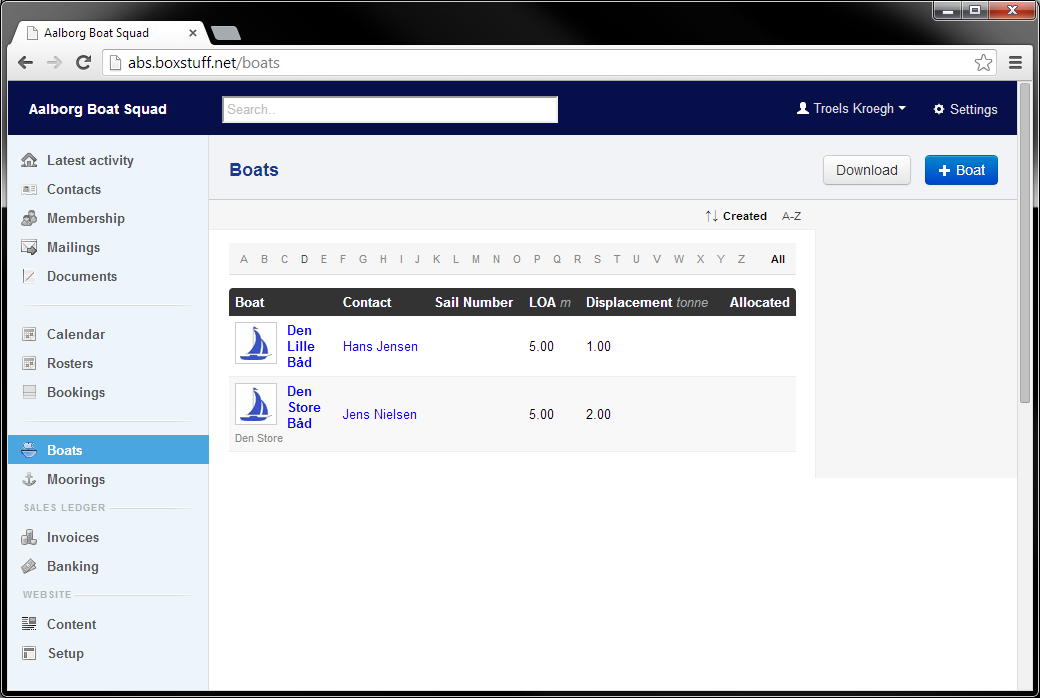
\includegraphics[scale=0.5]{images/teknologi/_Boats}
\end{figure}

\begin{figure}
	Personer som er en del af systemet, er en kontakt. De findes under /contacts.\newline
	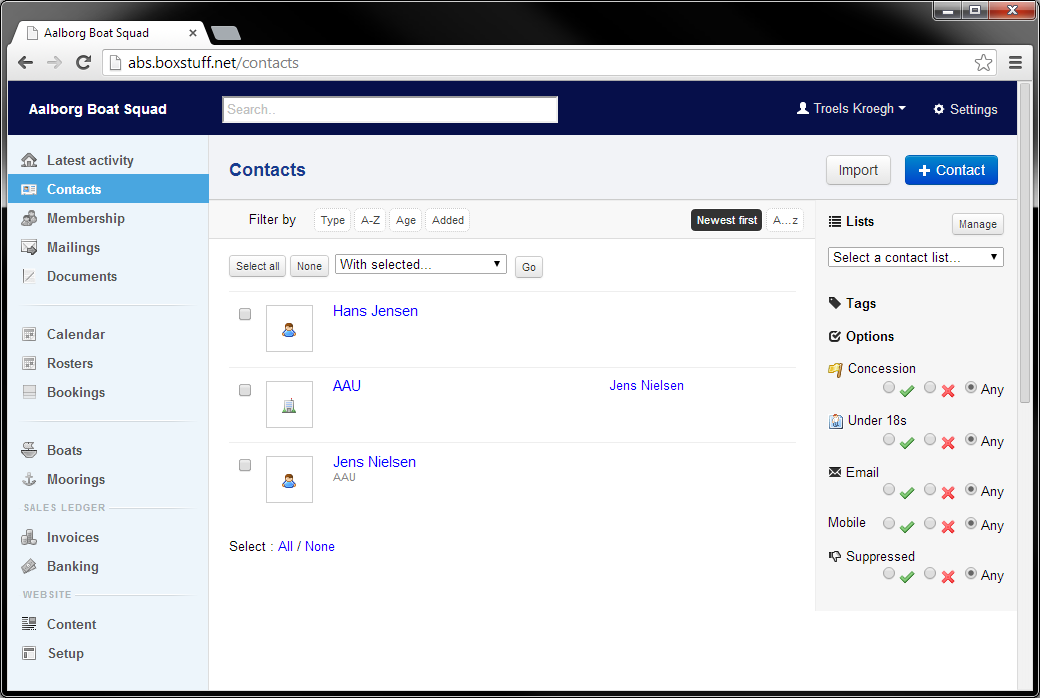
\includegraphics[scale=0.5]{images/teknologi/_Contacts}
\end{figure}

\begin{figure}
	Det er muligt at tilføje nye medlemmer, herunder hvilke type medlem de er. Disse typer er også muligt selv at lave i undermenuen Membership under /memberships/new.\newline
	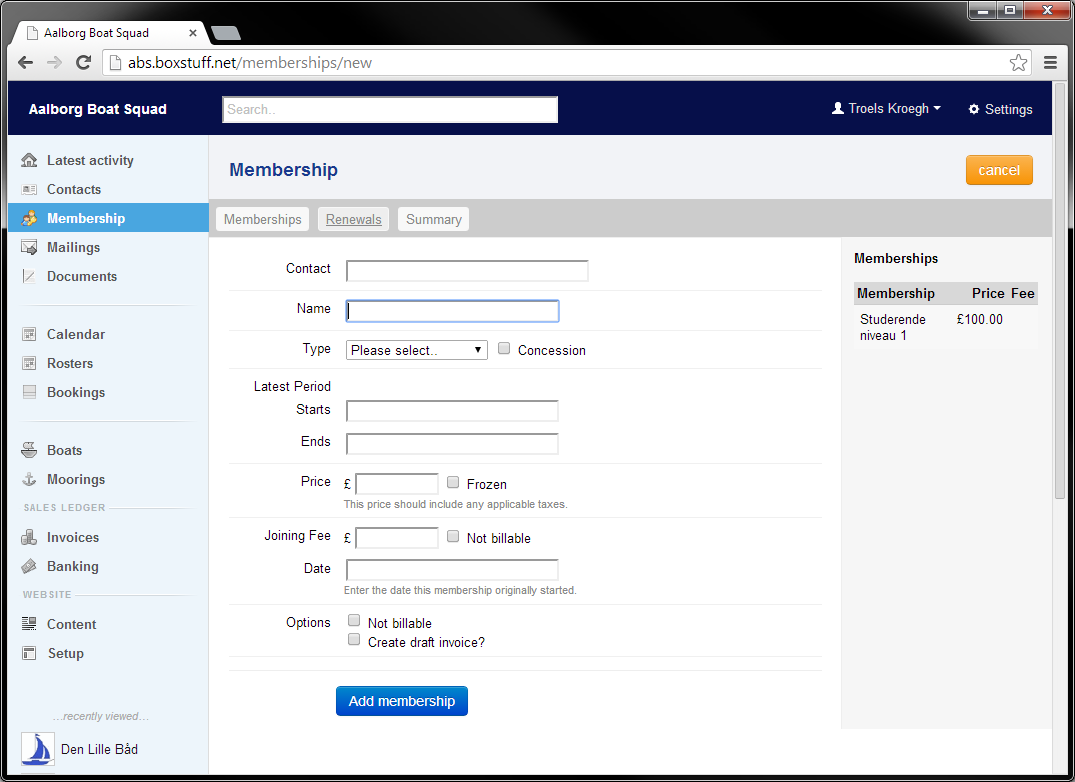
\includegraphics[scale=0.5]{images/teknologi/_AddMember}
\end{figure}

\begin{figure}
	Der findes en kalender med aktiviteter, som administratorer kan tilføje. Under /events.\newline
	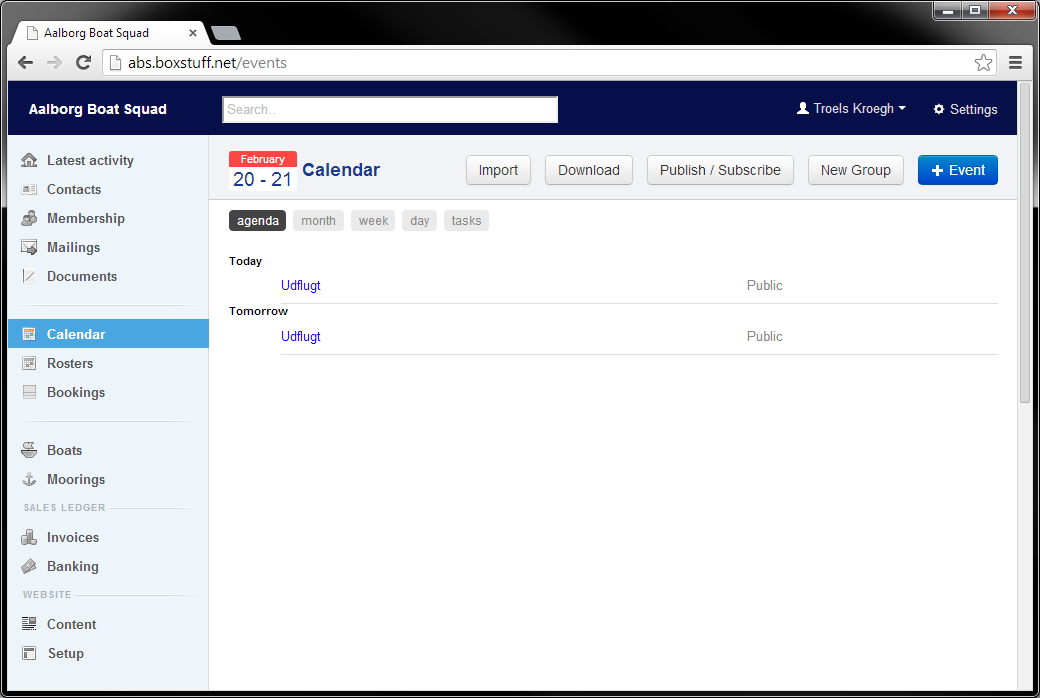
\includegraphics[scale=0.5]{images/teknologi/_Calendar}
\end{figure}

\begin{figure}
	Det er muligt for brugere at booke bådene, her har Hans Jensen booket en båd både den 20-02-2014 og den 26-02-2014. Dette findes under /booking/bookings.\newline
	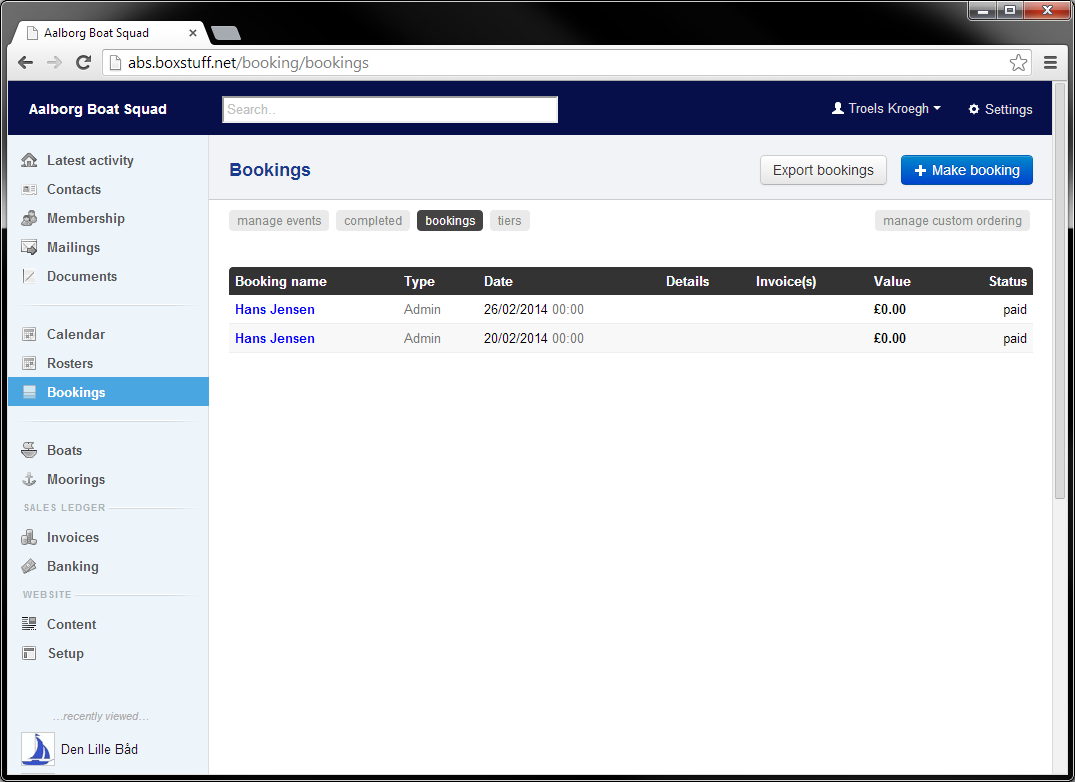
\includegraphics[scale=0.5]{images/teknologi/_Bookings}
\end{figure}

\begin{figure}
	Det er muligt at udskrive regninger baseret på brugeres udlån og kontingent. Under /invoices.\newline
	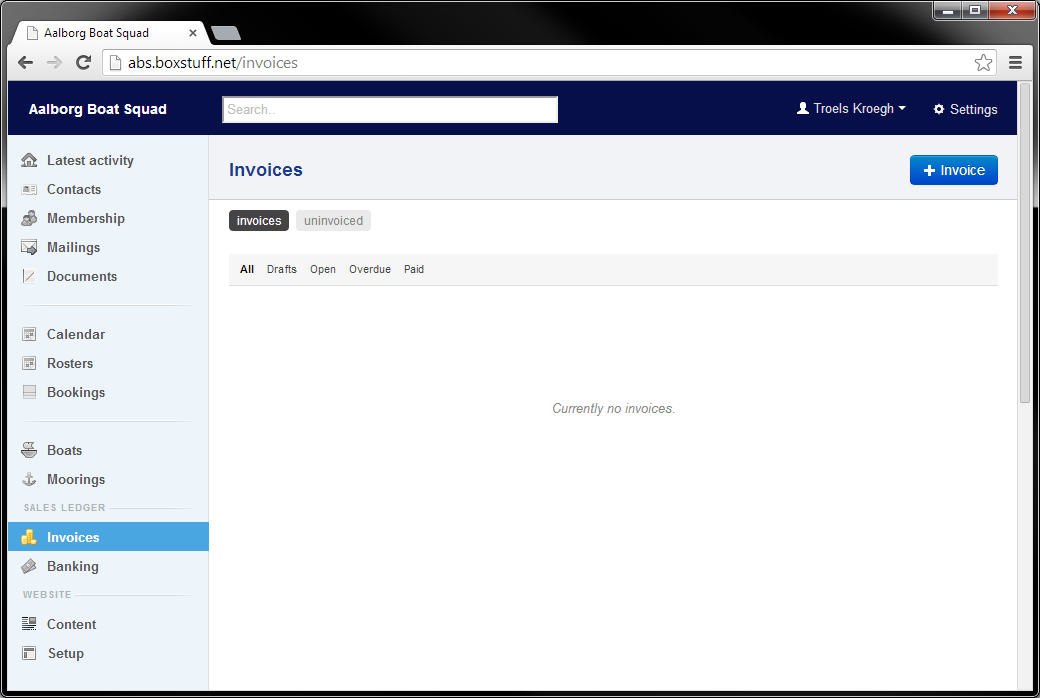
\includegraphics[scale=0.5]{images/teknologi/_Invoices}
\end{figure}


%\input{appendix/interview.tex}
\chapter{Interview Spørgsmål} \label{questions}
I dette afsnit ses de spørgsmål interviewet med Jacob Nørbjerg bygger på.

\begin{itemize}
\item Hvordan administrerer i sejlklubben lige nu(medlemmer, fartøjer og lign.)?
\item Hvilken information har i på jeres medlemmer(kvalifikation, niveau, erfaring eller lign)?
\item Hvor mange fartøjer har klubben selv til rådighed(sejlbåde, joller, ynglinge m.m.)?
\item Benytter i et EDB system til at administrere klubbens egne fartøjer?
	\begin{itemize}
	\item Hvis ja, hvilke egenskaber har systemet og hvordan kunne det forbedres?
	\item Hvis nej, hvordan administrerer i så fartøjer, og er i tilfredse med denne metode?
	\end{itemize}
\item Hvad er jeres største problem mht. administration af fartøjer?
\item Hvor meget tid anvendes der på administration af fartøjer(regninger, planlægning, vedligeholdelse osv.)?
\item Har i selv et vision om hvordan et system kan gøre det lettere for jer at styre ting i klubben (medlemmer, kontingenter, arrangementer, fartøjer osv.)?
\item Kan medlemmer leje/låne jeres fartøjer(joller, sejlbåde m.m.) når de ikke benyttes af sejlerskolen?
	\begin{itemize}
	\item Hvis nej, hvorfor tilbydes denne funktion ikke, er det noget der kunne tilbydes hvis der var et system til at hjælpe med administration?
	\item Hvis ja har vi et par ekstra spørgsmål herom:
		\begin{itemize}
		\item Hvad er kravene for at låne fartøjet?
		\item Hvordan håndteres omkostninger ved udlån af fartøjet?
		\item Hvordan administreres udlånte fartøjer og kunne hertil benyttes et system til hjælp? I så fald hvordan kunne et system bedst muligt være til hjælp?
		\end{itemize}
	\end{itemize}
\end{itemize}

\chapter{Interview transskribering}\label{bilag:interview-transkribering}
\textbf{Jacob}: I skal huske at det her baseret på muligvis forældet viden.

\textbf{Alle}: Jaja.

\textbf{Jacob}: Hvad mener i med at administrere i sejlklubben? Det er jo et bredt spørgsmål.

\textbf{Marc}: Det er primært hvordan i holder styr på de ting som ligger under sig.

\textbf{Jacob}: Vi har et hjemmestrikket medlemssystem. Det var jo den gang ikk'. Der ligger alt det sædvanlige ikk': Navn, adresse, telefonnummer. Så ligger der fuldt medlemsnummer og så ligger der ens uddannelse, altså sejlweskole, hvor langt man er kommet i forløbet på sejlerskolen og om man har førerbrevet, duelighedsbevis. Så ligger der om man er bådeejer, det koster nemlig flere penge. Der ligger vidst også noget om landpladsadminstration, alt hvad der hedder vand, plads i vandet, der organiserer havnen. Plads på land det arrangerer klubben. De klubber har forskellige landområder vi disponerer over. Det er så det generelle, det vi har på medlemmerne.
Så kan man, f.eks. hvis man som medlem har været... Hvis man skal betale for et eller andet, hvis man har lånt en båd og skal betale for det, så er der også et skærmbillede til det. Jeg kan ikke lige huske om man klikker direkte fra medlem eller man skal indføre medlemsnummeret der, men der er et sted hvor man kan gå ind og sige: ``Her er en der skal betale noget. Han skal betale for så og så mange dages leje af en båd og en motor osv. osv. og så printer vi en girokort ud.'' Det samme typisk skærmbillede bruger vi til: ``En som skal betale for en landplads og hans båd fylder så og så mange kvadratmeter dut [efterligner klikkelyd]''. Så kan man skrive ind her, som jeg gjorde i weekenden, lånte en af klubbens slibemaskiner med støvsuger og det koster så og så meget pr. dag, så meget af det ligger i et pr. accessbaseret tudsegammelt hjemmestrikket system som ligger på computeren nede i klubben.

\textbf{Søren}: Ligger det kun lokalt eller hvad?

\textbf{Jacob}: Ja, det ligger kun der lokalt og der er forskellige record udtræksningsmuligheder os' ikk: Gi' mig en liste over alle elever på andet år, gi' mig en liste over alle bådejere eller gi' mig en liste over hvilken rækkefølgen både skal sættes op i og sådan noget, så det er der også. Så har vi selvfølgelig senere, men det kan i se på nettet, så har vi jo indført forskellige... Altså meget af det information som vi kan trække det bliver så på forskellig vis smidt op på nettet. Det jeg sagde lige før med liste over hvornår både skal op den ligger på nettet, og den kan alle og enhver gå ind og se, så i kan gå ind og se hvad min båd hedder og hvornår den skal i vandet. Det ligger bare som en PDF. 
Nå, hvad har i på jeres medlemmer? [oplæsning af spørgsmål, spørgsmål var givet på forhånd] Der er sagt, altså vi har typisk om de har eller ikke har førerbrevet, om hvor langt de er kommet i skolen, hvis vi altså husker at vedligeholde det, det er ikke altid vi gør det. Det er vel sådan cirka det. 

Hvor mange både har vi til rådighed? [oplæsning af spørgsmål]

Ja det svinger meget. Den gang jeg var skolechef der havde vi 2 gaffelrigger, 3 drabanter og en spækhugger. Nu er konfigurationen ved at ændre sig lidt så nu hedder det stadig to gaffelriggere og så hedder det vidst nok to eller tre spækhuggere, er de ved at lave det om til og så nogle nye som hedder J80, sådan nogle satans små flyvepap. Jeg tror de unge mennesker kommer til at få nogle forskrækkelser når de skal ud og sejle dem første gang hvis de ikke har sejlet før, men det er jo deres problem. Det er jo en politisk diskussion. Og så har vi en enkelt yngling. Det var en som blev til overs engang, den er bare blevet foræret til klubben. Den er til at læren til at lege i og så har faktisk en fire... men de er ikke rigtig taget med der, vi har en fire til seks Mini12'er, hedder de. Det er til handicapafdelingen. De ligner gammeldags Americas Cup både som de så ud den gang de lignede sejlbåde, skaleret ned i en to-tre meters længde, så kan man sidde nede i dem og styre med hænderne eller fødderne eller hvad man har at bruge, så den bruger handicap-afdelingen til når handicappede er ude og sejle. 

Et EDB-system? [oplæsning af spørgsmål]

Ja, i den forstand at vi har overblik over hvilke både vi har. Så er der kommet det der online reservationssystem, men den situation jeg kendte, som jeg tror stadig ligger bagved, fordi der kan man kun reservere en båd, det er jo at der inde i skolestuen, dvs. det er der hvor der ligger redningsveste og grej til alle bådene og sådan, der ligger der en stor bog hvor man går ind og skriver ``3. maj, sådan og sådan, Jacob, besætning, telefonnummer på Jacob, hvornår sejler vi, hvornår tror vi at vi kommer hjem, hvor tror vi nok vi tager hen'' og så et eller andet sted, en kolonne som hedder: Det var her vi kom hjem, og hvis der er nogen kommentar, så det er sådan en stor bog af den tykke der, den fylder sådan her [viser hvor står bogen er]. 
Så er der på hver båd en havariprotokol, dvs. at hvis der er et eller andet med båden, så tager man den rigtige bog frem og skriver: ``Jeg var ude og sejle med båden og jeg smadrede ind i Oslobåden'' eller et eller andet, der var noget som knækkede, sejlede revnede eller hvad det nu var og hvis man ikke kan reparere det selv så skriver man det der. Hvis man føler eller ved at det er noget som bare skal repareres i en helveds fart, så er man stærkt opfodret til at ringe til skolechefen eller den der har ansvar for båden. Hver båd har en bådchef der er ansvarlig på den båd, så hvis man kan se at det her kræver mere end jeg lige kan klare, det kræver noget værktøj, reservedele, det kræver måske syn af en bådbygger, så skal man så ringe til den pågældende person som så vil sætte det i værk. Hvis man kan reparere det selv så prøver man også på at gøre det, men bare lige skriv et notat om at der var noget eller hvis det er noget som skal laves, men det kan godt sejle uden det laves så skriv det lige. 

Så er der skolen: Hver båd hver aften har sådan et fortrykt ark: Fører, elever, sejladsnummer, dato, afkrydsning, hvem og hvad. Ud fra hver, mulighed for bemærkning: Skete der et eller andet, hvad gjorde vi, er der nogen som ikke dukker op, er der gæster med så bliver de også bare skrevet på der nedenunder den faste liste, og hvis det er en anden fører skriver man også det på, så krydser man af den aften det handlede om og det bruget man tildels til at holde øje med hvem der kommer, hvem der ikke kommer, hvem som husker at melde afbud, og glemmer det, det er fyfy at glemme at melde afbud, og tælle op antal gange man har sejlet, det er jo også vigtigt, altså i forhold til proportion på skolen, det var sejladsprotokollen til skolen. 

Så har vi selvfølgelig reservationssystemet, som flytter lidt der, men der er stadig sådan et andet slags reservationssystem som handler om når skolen arrangerer noget. Når skolen siger: ``Nu på første weekend i juni der er der 24-timers sejlads, det er en skide god oplevelse. Er der nogen elever der gerne vil være med?'' Så hænger der gerne sådan et stykke papir nede i gangen hvor der står 24-timer sejlads, her kan førerne skrive sig på og her kan eleverne skrive sig på og så må man håbe at der er nogen som skriver sig på. Så det er sådan en: ``Her er et tilbud om en ekstra tur af en eller anden slags, skriv jer lige på her.'' Det foregår også på papir. Så det kræver altid at man kommer der ned og gør noget, skrive sig på, sørge for overblik. Så det der *pullik 9:11* der hedder ``Hvad er jeres største problem'', det største problem jeg oplevede var simpelthen det her med at holde styr på... Som administrativ ansvarlig, så er der bare en fandens masse papir som man skal holde styr på. Man skal ind og tælle op på den der mødeliste, man skal... Den gang skulle man hvis nogen ringede ned og sagde kunne jeg reservere en båd på det og det tidspunkt, så skulle man ud og finde... Vi havde gerne sådan en kalender hængende nede på opslagstavlen med bådene og datoerne, så kunne man så blive krydset af, enten gjorde folk det selv eller så bad de os om at gøre det. Havde anden kalender bl.a. seddel som hang der med reservation til onsdags-kap-sejlads, sådan at folk ``Jeg vil gerne ud og sejle onsdags-kap-sejladsen i næste uge'' så skriver man sig lige på, ``jeg har reserveret båden'' og den der første når frem med en kuglepen har vundet og enten skriver man ``jeg har besætning'' eller ``jeg har plads til to elever'' eller hvad det nu er og så må folk finde ud af det på den måde. Det kræver igen at man kommer ned og kigger på opslagstavlen og forstår det der. Der var en regel omkring onsdagsmatch med at man kun kan reservere en ude ud i forvejen. Det der med at man bare lige, nogen af de gamle, der er altid nogen som sejler onsdagsmatch rundt i vores både de tager blokreservation hen over hele sommeren, nænæ. Man kan reservere en uge i forvejen. Det er jo en politik, som man har. 

Det er meget papirarbejde. Når man skal finde ud af hvor meget der skal betales, så skal man ind i den store [bog] og så skal man ind og se hvem har egentlig lejet en båd og så gå igennem, og så skal man jo prøve på... Typisk så gør man det måske tre-fire gange i løbet af en sommer, maks. Dvs. at man skal finde alle de gange hvor den person har haft fat i båden, og hvad er det: En aften, en dag, en weekend, hvad fanden er det for noget? 

\textbf{Marc}: Krydsrefereres om der er elever med? 

\textbf{Jacob}: Ja det kan man... Det er vel den nye politik, så skal man også finde ud af om der er elever med. Det tror jeg nok vi havde en... [politik]. Så indførte vi en da det kom så indførte vi med at man lige kunne lave et kryds på besætningen og sige at man har en elev med eller skrive et sted at man har en elev med, så skal man også lige finde ud af det. Så gik vi ikke mere ned i det end at vi stolede på, at hvis man skrev at man havde en elev med, så stolede vi på det. [eksempel:] Nå det var så Anette, hun har jo sejlet der, nå er han blevet stillet ind: fint. Og så gå igennem sådan 2-3 sider, der bliver hurtigt fuldt op på sådan en side så, fandens besvær, derfor gad vi heller ikke gøre det til sidst. 
Og så blev der skrevet girokort ud som blev puttet i en kurvert og sendt til den pågældende. Nogen af os kunne godt finde ud af at fiske girokortet over i en PDF og så bare få det sendt på mail, men som regel blev det noget med en kuvert. ``Ikke nogen elektronisk opkræven her.'' 

Hvis vi går sådan lidt længere ud... Så omkring det hele med skolen, men det er nok lidt voldsomt, der synes jeg at det havde været et kæmpe puslespil det med at få styr på hvilke elever skal være hvor og hvilke dage og hvordan får vi placeret dem på både osv. Men problemet var ofte lige så stort... Skyldtes lige så meget at folk bare ikke fik meldt tilbage når vi skrev: Nu må i godt lige få sendt jeres ønsker. Når vi skriver til folk: ``Nu skal vi lige have af vide: Om du har tænkt dig at sejle til sommer, om du sidder over et år eller hvad du gør, hvilke dage du kan sejle.'' Og hvis de ikke kommer så sidder man bare der... Man kan ikke lave planen. Det synes jeg at vi brugte meget tid på, vi havde ikke rigtig noget støtte til at lave den der [plan], det blev sådan et Excel-regneark til sidst, med båd og elever og så blev det bare hængt op på opslagstavlen: Sådan her ser det ud. Det var sådan lidt... Det virkede.
Som elev og som medlem synes jeg at det største var det besværlige med man kan bare ikke få overblik over en skid hjemmefra. Altså hvilke både er ledige? Det kan så se med det nye system som de har lavet, men jeg kunne virkelig godt tænke mig at sejle 24-timers sejlads. Der skal man altså have fat i *et eller andet 13:58* nede i Sundet og bede om: Er den der indkaldelse kommet op og hænge. Jeg vil gerne ud og sejle onsdagsmatch, der kan man så gå igen. Jeg vil gerne faktisk finde ud af om der er en ledig plads på en onsdagsmatchbåd. Altså, en ting er om den er reserveret, en anden ting er om der lige er en er en... ``Kan jeg lige springe på som besætning her.'' Så den der manglende afgang til information når man sidder der hjemme og gerne vil et eller andet og så det der med at det hele er papirbaseret. Skulle gå igennem en stor protokol for at finde ud af hvad folk skal betale for et eller andet, det må da kunne gøres smartere. Min vision var den gang noget integration mellem de forskellige ting, mellem brug af både til skole, til fritidsbrug, til kapsejlads, til skolearrangeret fritidsbrug. Altså der er forskel på at jeg beslutter tage ud søndag og sejle med nogle venner og så at skolen siger at den søndag er der et arrangement som skolen gerne vil ha' at kommer ud, så der laver skolen nærmest en *for-et-eller-andet 15:17*, som så først bliver oplyst måske tre dage før at man finder ud af at der kommer noget, så bliver båden frigivet. Så der er det igen med at man som medlem kan gå ind og se: Kan man komme til der. For det er forskellig måder at reservere og bruge en båd på som godt kan være lidt indviklet at finde rundt i. 

Som medlem kan man leje og låne et fartøj? [oplæsning af spørgsmål]

Ja det kan de sagtens. Det ved i godt. Kravene er førerbeviset. Omkostninger: Vi sender et girokort. Administreres: Ja det gør de jo stortset ved at vi har de der papir, protokoller hvor man skriver sig i. 

\textbf{Søren}: Det der førerbevis det får man bare igennem skolen på de to år som det tager eller er det kun duelighedsbeviset?

\textbf{Jacob}: Altså det tager to år på skolen, det er på den måde vi organiseret det på. Det er et valg man har truffet i klubberne der nede. Jamen det tager to år og faktisk har de tre klubber en lidt forskellig policy omkring det, men i Sundet har det været sådan, *der siges et eller andet 16:35*, det var sådan at det første år sejlede man med yoghurtbærger, undskyld plastikfiberbåde og det andet år sejlede man gaffelriggere. Og det ud fra sådan rent propertion, altså glasfiber, sådan en drabant der, den skal men for det første være rigtigt ond ved den før den vælter og for det andet så er den forholdsvis nem at sejle og man får meget klar og hurtig besked hvis man gør noget forkert, båden giver meget hurtig tilbagemelding. Gaffelriggeren er  svær, den er tung, den er længere om at reagere, den gir' ikke så hurtig og klar besked om hvad der foregår, dvs. at man skal være mere erfaren for at forstå hvad den fortæller en. Så den prøver vi på ikke at skræmme førsteårseleverne i. Alene mængden at torvværk det ku' godt få folk til at blive bekymrede når de sådan skal finde ud af det. Set enkelt er det en fantastisk båd at undervise i, den har et stort åbent...[plads] Man kan gå rundt nede i den. Man sidder ikke sådan klemt sammen på smalle bænke, man kan gå omkring, fedt. Så det tager to år. Så har vi, nu glemte jeg at sige før med Spækhuggeren, jeg sagde vi havde en Spækhugger, vi har skolen 2 år. Så har vi det der hedder... Det er så blevet en kapsejladsskole, sammen med de andre klubber i havnen, så folk der er blevet uddannet fra sejlklubberne, kan så tilmelde sig kapsejladsskolen, dvs., det er mest spækhugger vi gør det i, dvs. så kommer de... Så for det noget teoriundervisning og noget praksisundervisning i kapsejlads på forskellige niveauer kulminerende med at man så kan deltage i almindelig kapsejlads. Det er ikke noget man skal, lige så snart man har førerbeviset, så kan du gå ud og sejle kapsejlads, det er slet ikke det, men der er mange der godt vil have den der uddannelse, forstå hvordan man *et eller andet med start 18:33*, hvordan lægger man taktik, hvordan får man samarbejdet til at fungere, til kapsejlads skal det gå temmelig stærkt, så det har vi så sammen med de andre, det er så os klubben, så spækhuggeren, den ene og muligvis også den næste, er mere eller mindre fastreserveret til kapsejladsskolen mandag, tirsdag og onsdag tror jeg det er. Så det er jo også en anden fast ting, altså hvor vi har... Faktisk bliver de jo... Den protokol de udfylder er den samme som skoleprotokollen, den er fortrykt med navne på, afkrydsning, du er på dette kapsejladshold, på den båd om mandagen. Så må du krydse af når du kommer. Og det her med at vi hvem der er på båden det er jo i forhold til skolen, i forhold til skolens regler for om man er dygtig nok når man har gjort nok, og det er helt generelt at vi vil vide hvem som er på båden, altid, når den er ude og sejle, det er rent sikkerhedsmæssigt. Så det har det dobbelte formål. 

\textbf{Søren}: Ja det var...

\textbf{Jacob}: Har jeg fået svaret på alle jeres spørgsmål? Jeg kørte bare der ud af. 

\textbf{Alle}: Ja det tror jeg.

%\chapter{UML-diagram}\label{UML_diagram}

\begin{figure}[htbp]
  \centering
  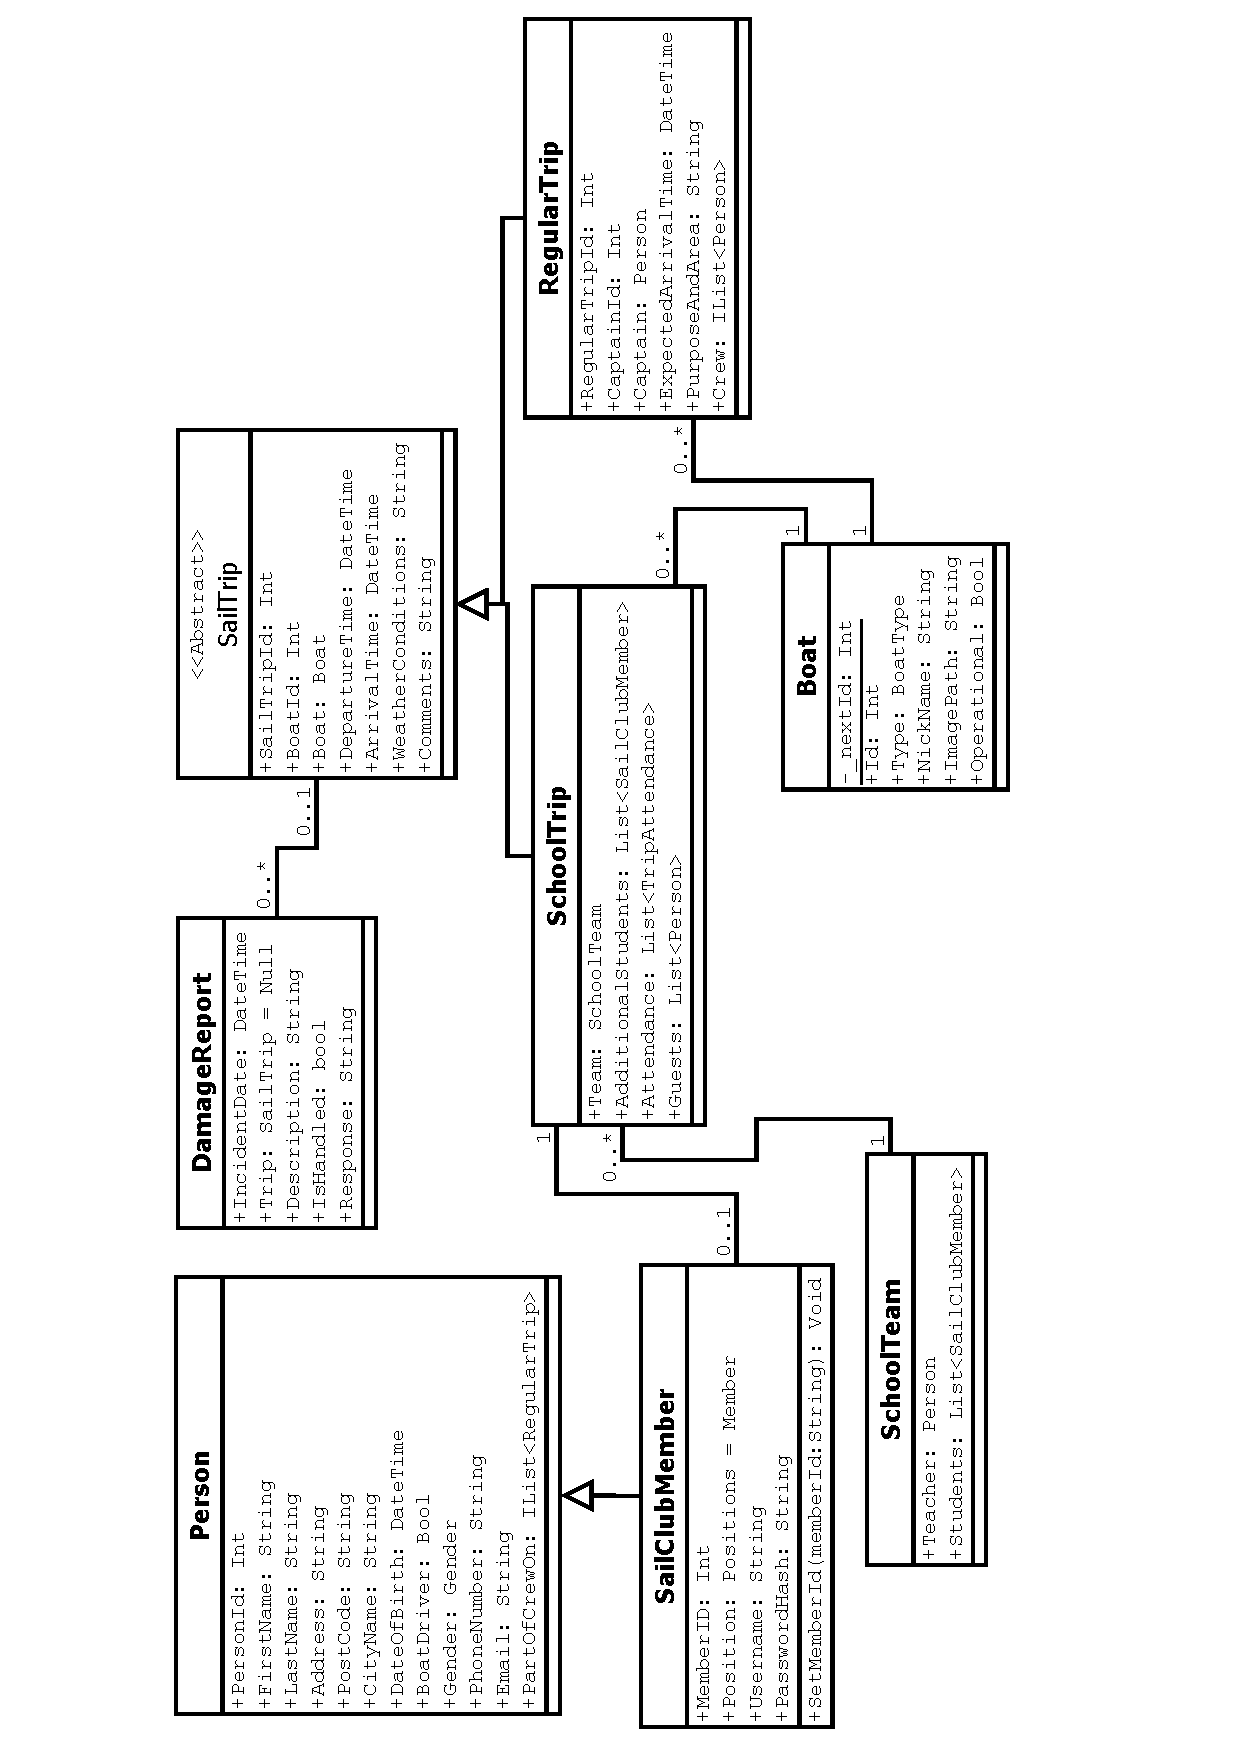
\includegraphics[width=0.75\textwidth]{images/flowcharts/UML.pdf}
  \caption{UML-diagram over klasserne i projektets program}
  \label{fig:UML}
\end{figure}
%\chapter{Use Cases}\label{Use_cases}
\cbstart
\textbf{Case 1:}

En bruger af systemet ønsker at komme ud og sejle. Brugeren logger ind på systemet med sit personlige login. Han navigerer ind på bookingsiden. Han vælger sin foretrukne båd og vælger datoen for hans booking. Han gennemfører bookingen og logger derefter ud af systemet.

\textbf{Case 2:}

En bruger som har været ude og sejle logger ind på systemet. Han ser på sin forside at han mangler at udfylde logbogen for den sejltur han lige har været på. Han vælger logbogen og trykker udfyld. Vinduet hvor han skal udfylde de resterende informationer popper op, og han udfylder felterne. Han trykker derefter på gem log, og logger ud af systemet.

\textbf{Case 3:}

En administrator har fået at vide at en båd er blevet skadet under en sejlads. Han logger ind på systemet og navigere ind på den pågældende båds side. Han åbner logbogen for bådens seneste tur og ser at båden er skadet. Han skriver en kommentar til logbogen, hvori han skriver at skaden vil blive udbedret indenfor kort tid. Administratoren logger derefter ud igen.

\cbend
\chapter{Bruger tests af program}\label{BrugerTestCases}

Du skal nu teste programmet vi har udviklet i forbindelse med vores P2-projekt på AAU. Programmet er lavet som et management system til en sejlklub, så de kan holde styr på deres både, deres medlemmer, deres undervisningsforløb, og desuden deres logbøger de holder for alle klubbens både. I den forbindelse vil du blive bedt om at udføre forskellige opgaver i vores program. Et eksempel kunne være at vi beder dig logge ind med et givent brugernavn og kodeord, og herefter finde frem til medlemmet Troels Kroegh, i medlemsoversigten.

Hvis der er noget du kommer i tvivl om, f.eks. hvad du skal i den givne opgave, så kan du spørge, og vi vil vurdere om det vil ødelægge testen at få svaret på dit spørgsmål.


\section{Opgave 1}

Log ind med følgende brugeroplysninger: 
\newline - Brugernavn: kasper
\newline - Kodeord: eriksen

Når du har gjort dette bedes du finde tilmelde dig begivenheden " Pizza Fest" som finder sted den 20/6-14  klokken 19.00.

\section{Opgave 2}

Forbliv logget ind til denne opgave. Du bedes nu booke en båd med følgende oplysninger:

\begin{itemize}
	\item Bådnavn: Anastasia
	\item Besætning: 
	\begin{itemize}
		\item Lars Olsen
		\item Karen Wolff
		\item Bodil Kjær
		\item Anne Frank
	\end{itemize}
	\item Kaptajn: Anders And
	\item Formål: " Vi skal ud og fiske på havet."
	\item Afgang: " 20/6-14 klokken 09:00 " 
	\item Ankomst " 20/6-14 klokken 17.00 "
\end{itemize}

Log herefter ud af programmet, så du er klar til næste opgave, som du finder på næste side.

\newpage
 
\section{Opgave 3}

Log ind med følgende brugeroplysninger: 
\newline - Brugernavn: oskar
\newline - Kodeord: lauridsen

Dette medlem er administrator da medlemmet er en af sejlerskolens undervisere.
Du har lige været ude og undervise eleverne og skal nu registrere at dit hold har fuldført et nyt punkt på deres liste over mål i forbindelse med uddannelsen.

Du bedes 

\begin{itemize}
\item Finde holdet: Svenskerne
\item Vælg lektion: 05/09/2014 kl. 15:00 \fxnote{Kunne ikke åbne programmet da jeg lavede det her så er ikke sikker på formatet}
\item Afkryds at alle medlemmer på holdet har fuldført deres natsejlads
\item Gem herefter lektionsinformationerne
\end{itemize}


\section{Opgave 4}

Forbliv logget ind til denne opgave.

Gør følgende:
\begin{itemize}
\item Vælg hold: Svenskerne
\item Opret lektion for holdet der starter kl. 19.00 og slutter kl. 21.00 den 1. august 2014
\end{itemize}


\section{Opgave 5}

Forbliv logget ind til denne opgave.

Her skal du:
\begin{itemize}
		\item Opret et nyt hold
		\item Navngiv holdet: TestHold
		\item Holdet skal bestå af følgende medlemmer: 
		\begin{itemize}
			\item Isabella Christensen
			\item Malthe Frandsen
			\item Malene Jensen
			\item Josefine Henriksen
		\end{itemize}
		\item Holdet skal være et andenårs hold 		
		\item Gem nu holdet i programmet
\end{itemize}

\section{Opgave 6}

Forbliv logget ind til denne opgave.

Holdet 'MasterRace' \fxnote{Alle eleverne på holdet skal have sat alle læringsområderne til true} har færdiggjort alle læringsområderne, så de kan nu få et bådførerbevis.

For at opnå dette, gør følgende
\begin{itemize}
\item Vælg hold: MasterRace
\item Forfrem holdet
\end{itemize}


\section{Opgave 7}

Forbliv logget ind til denne opgave.

Du bedes:
\begin{itemize}
\item Vælg hold: TestHold
\item Slet holdet
\end{itemize}


\section{Opgave 8}

Inden du logger ud fra administratorbrugeren bedes du oprette en ny begivenhed.

Begivenheden skal foregå den 7/6-14, og skal hedde, Bålfest ved molen. Beskrivelsen kan være hvad som helst, alle kan tilmelde sig. Log herefter ud igen.


\section{Opgave 9}

Log ind med følgende brugeroplysninger: 
\newline - Brugernavn: michelle
\newline - Kodeord: kristensen

Dette medlem en elev. Du er færdig med de to års sejlskole og vil være sikker på at du kan få dit bådførerbevis.

Tjek derfor at alle læringsområderne er tjekket af.

Log herefter ud af programmet.


\section{Opgave 10}

Log ind med følgende brugeroplysninger: 
\newline - Brugernavn: marcus
\newline - Kodeord: husmand

Du er nu kommet hjem fra en sejltur og skal udfylde din logbog for turen.

Turen foregik den 18/6-14, og havde formålet: "Sejler til Sverige og hjem igen."

Find logbogen frem og udfyld felterne, efter egen fantasi. (Du får ikke oplyst informationerne her, du skal altså selv finde på noget at skrive. Det behøver ikke give mening.)

Når du har gjort dette vil vi bede dig finde frem til din nu udfyldte logbog. 

\section{Testen er nu slut}


Tak fordi du ville være med i vores test, vi har nogle opfølgende spørgsmål som vil blive stillet til dig af observatøren fra vores gruppe.

\fxnote{Her skal være bedre beskrivelse af både opret event samt undervisning, jeg kender ikke nok til funktionerne i har lavet.}


\chapter{Database}\label{bilag:SporgeSkema}
Spørgeskema for brugertests af programmet.

\textbf{På en skala fra 1-5 hvor overskueligt synes du så programmet var at navigere rundt i?}

[1 er meget uoverskueligt, og 5 er meget overskueligt.]

\begin{itemize}
\item Vurdering: 
\item Hvorfor denne holdning? 
\item Hvilke elementer tænker du specifikt på?
\end{itemize}

\textbf{På en skala fra 1-5, hvor let var det at overskue et skærmvindues funktionaliteter?} - Se tabellen nederst på siden.

[1 er meget svært, og 5 er meget let.]

\begin{table}\label{TabelVurdering}
    \begin{tabular}{l|l|l}
    ~                       & Vurdering & Kommentar \\ \hline
    Forside                 & ~         & ~         \\
    Undervisning            & ~         & ~         \\
    Medlemmer               & ~         & ~         \\
    Både og Booking         & ~         & ~         \\
    Begivenheder            & ~         & ~         \\
    Logbogsvinduet          & ~         & ~         \\
    CreateCrewWindow        & ~         & ~         \\
    CreateBoatBookingWindow & ~         & ~         \\
    \end{tabular}
\end{table}

\textbf{Var der noget ved programmet du ikke forstod?}

\textbf{Var der noget der fungerede godt?}



\textbf{Hvad fungerede mindre godt?}

\textbf{Hvis du kunne ændre noget på programmets udseende eller navigering, hvad ville det så være?}

\textbf{Har du nogle forslag eller tanker om programmet?}

% Insert each appendix under this



%%%%%%%%%
% INDEX %
%%%%%%%%%

\newpage
\printindex

\end{document}
